% !TeX encoding = UTF-8
\documentclass[12pt,letterpaper,oneside]{book}
\usepackage[utf8]{inputenc}
\usepackage[spanish, mexico]{babel} %Para poner el texto generado por LaTeX en español
\usepackage{graphicx} %Para importar imágenes
\usepackage[hidelinks]{hyperref} %Para incluir hiperenlaces en el texto
\usepackage[numbers]{natbib} %Para soportar citas numéricas
\usepackage{babelbib}
\usepackage{algorithmic} %Para escribir algoritmos con pseudocódigo con el entorno algorithmic
\usepackage{listings} %Para escribir código fuente
\usepackage[usenames,dvipsnames,svgnames,table]{xcolor} %Para soportar el uso de colores en el texto, si se requiere, de lo contrario se quita
\usepackage[left=2.50cm, right=2.00cm, top=2.15cm, bottom=2.15cm]{geometry} %Para cambiar los márgenes
\pagestyle{plain}
%\usepackage{fancyhdr} %Para modificar los encabezados de las páginas
\usepackage{lipsum} %Para el comando de relleno lipsum, recuerda eliminarla cuando ya estes trabajando en tu tesis
\usepackage{booktabs} %Para incluir líneas horizontales en las tablas especiales para libros (con los comandos \toprule, \midrule y \bottomrule)
\usepackage{amsmath} %Para soportar el entorno matrix
\usepackage{amssymb} %Para símbolos matemáticos como \mathbb
\usepackage{pgfgantt}  %Para calendario de actividades (gráfica de gantt)
\usepackage{tikz}
\usetikzlibrary{positioning, arrows.meta, fit, backgrounds, calc}
\usepackage{placeins} %Para \FloatBarrier: evita que tablas/figuras crucen límites de sección
% \usepackage{natbib} 


\renewcommand{\baselinestretch}{1.5} %interlineado
%\setcounter{secnumdepth}{3} %niveles a considerar en el índice (capítulo, sección, subsección,)
\author{}
\title{}

\newcommand\BackgroundPic{
	\put(0,0){
		\parbox[b][\paperheight]{\paperwidth}{%
			\vfill
			\centering
			\includegraphics[width=0.9\paperwidth,height=0.9\paperheight,
			keepaspectratio]{img/fondo.png}%
			\vfill
}}}
\graphicspath{{img/}{./}}
\begin{document}
	%Capítulo frontales o de introducción (no se pagina igual que el resto):
	\frontmatter
	%Portada 
	\begin{titlepage}
		\sffamily
		%\AddToShipoutPicture*{\BackgroundPic} esta versión no tiene fondo de agua
		\noindent
		\begin{minipage}{0.30\textwidth}
			\begin{flushleft}
				\noindent\includegraphics[width=1.3\linewidth]{img/sep2021.png}
			\end{flushleft}
		\end{minipage}
		\begin{minipage}{.45\textwidth}
			\begin{center}
				\noindent
\includegraphics[width=.5\linewidth]{img/TecNM.png}
			\end{center}
		\end{minipage}
		\begin{minipage}{.25\textwidth}
			\begin{flushright}
				\noindent
\includegraphics[width=.5\linewidth]{img/logotec.png}
			\end{flushright}
		\end{minipage}
		
		\begin{center}
			\normalsize
			\vspace*{2.5cm}
			INSTITUTO TECNOLÓGICO DE LA PAZ\\[-0.3cm]
			DIVISIÓN DE ESTUDIOS DE POSGRADO E INVESTIGACIÓN\\[-0.3cm]
			MAESTRÍA EN SISTEMAS COMPUTACIONALES\\[1cm]
			
			\Large
			\textbf{LOGÍSTICA DE ÚLTIMA MILLA EN REDES VIALES REALES: UN ENFOQUE REPRODUCIBLE PARA EL MDRP EN LA PAZ, B.C.S.}\\[1cm]	
			\textbf{ANTEPROYECTO DE TESIS}\\[1cm]
			\large
			QUE PARA OBTENER EL GRADO DE\\[-0.3cm]
			MAESTRO EN SISTEMAS COMPUTACIONALES\\[1cm]
			
			\normalsize
			PRESENTA:\\[-0.3cm]
			\large ALAN JOSÉ MARCOS SÁNCHEZ MARTÍNEZ\\[1cm]
			
			\normalsize
			DIRECTORES DE TESIS:\\[-0.3cm]
			\large DR. MARCO ANTONIO CASTRO LIERA\\[-0.3cm]
		\end{center}
		\begin{flushright}
			\normalsize
			LA PAZ, BAJA CALIFORNIA SUR, MÉXICO, DICIEMBRE 2023.
		\end{flushright}
	\end{titlepage}
	\vspace*{\fill}
	%para "apagar" el número de capítulo
	\makeatletter
	\renewcommand{\thesection}{%
		\ifnum\c@chapter <1 \@arabic\c@section
		\else\thechapter. \@arabic\c@section\fi}
	\makeatother
	%Índice general de contenidos
	\tableofcontents
	
	%Lista de figuras, si la escuela lo requiere
	\listoffigures
	
	%Lista de tablas, también opcional
	\listoftables
	
	%Capítulos de contenido, estos llevan la paginación normal
	\mainmatter
	
	
	\chapter{Introducción}

\section{Antecedentes}

\subsection{De TSP a VRP}
El Problema del Vendedor Viajero (TSP, por sus siglas en inglés) es uno de los problemas de 
optimización combinatoria más estudiados y fundamentales en la investigación de operaciones. 
En su forma más simple, el problema busca determinar el recorrido más corto posible que visita 
un conjunto de ciudades exactamente una vez, comenzando y terminando en la misma ciudad. 

A pesar de su sencilla definición, el TSP es NP-duro, ya que el tiempo requerido 
para encontrar una solución óptima crece factorialmente con el número de ciudades, haciendo 
que las instancias de gran tamaño sean computacionalmente intratables para métodos exactos \citep{Lenstra1981}.

El TSP sirve como pilar para una clase más amplia y práctica de problemas de logística: 
el Problema de Enrutamiento de Vehículos (VRP). La transición conceptual del TSP al VRP 
ocurrió con el trabajo seminal de \citet{Dantzig1959}, quienes formularon "The Truck Dispatching 
Problem". Este trabajo generalizó el TSP al considerar una flota de vehículos con capacidad 
limitada, con el objetivo de servir a un conjunto de clientes desde un depósito central. 
Esta generalización marcó el nacimiento del VRP, que busca minimizar el costo total de las 
rutas (usualmente en términos de distancia o tiempo) para una flota de vehículos que atiende 
a un conjunto de clientes con demandas conocidas.

Al igual que el TSP, el VRP es NP-duro \citep{Lenstra1981}, pero su estructura es significativamente
más rica y compleja. La complejidad no solo reside en encontrar las secuencias óptimas de visitas 
(como en el TSP), sino también en asignar clientes a vehículos y rutas de manera eficiente \citep{Caceres-Cruz2014}. A lo 
largo de cinco décadas, el VRP ha evolucionado para incorporar una gran variedad de restricciones 
del mundo real, dando lugar a los llamados "Rich VRPs" \citep{Caceres-Cruz2014}. Estas extensiones 
incluyen, entre otras:

\subsection{VRP clásico y extensiones con restricciones } % Dantzig1959, Caceres-Cruz2014, Laporte2009VRPSurvey

\begin{itemize}
	\item \textbf{Capacidades de los vehículos (CVRP)}: Donde cada vehículo tiene una capacidad 
	máxima de carga que no puede ser excedida. El CVRP introduce la decisión adicional de no solo 
	determinar la secuencia de visitas, sino también decidir cuánto llevar en cada viaje, 
	lo que aumenta significativamente la complejidad computacional del problema. Cada vehículo debe 
	partir desde un depósito central y retornar a él, respetando siempre la restricción de capacidad \citep{Caceres-Cruz2014}.
	
	\item \textbf{Ventanas de tiempo (VRPTW)}: Donde cada cliente debe ser atendido dentro de un 
	intervalo de tiempo específico. Las ventanas de tiempo añaden complejidad porque no solo se optimiza 
	la distancia de las rutas, sino también el tiempo, considerando que los vehículos pueden llegar 
	temprano (y esperar con costo de tiempo de espera) o llegar tarde (incurriendo en penalizaciones). 
	Esta restricción introduce la dimensión temporal explícita al problema de enrutamiento \citep{Caceres-Cruz2014}.
	
	\item \textbf{Múltiples depósitos (MDVRP)}: Donde los vehículos pueden iniciar y terminar sus rutas
	desde diferentes ubicaciones, en lugar de un único depósito central. Esto introduce complejidad 
	adicional porque el algoritmo debe decidir no solo las rutas de visita, sino también asignar 
	qué vehículos operan desde qué depósitos. El MDVRP es relevante en contextos logísticos donde 
	múltiples centros de distribución sirven diferentes regiones geográficas \citep{Caceres-Cruz2014}.
\end{itemize}

Más allá de estas extensiones fundamentales, la literatura identificada en \citet{Laporte2009VRPSurvey} 
documenta otras variantes relevantes, como problemas con \textit{pickup} y \textit{delivery} (recogida y entrega en diferentes 
ubicaciones), problemas con \textit{splits} de demanda (dividir la demanda de un cliente entre múltiples vehículos) y 
problemas con tiempos de servicio variables. Cada una de estas extensiones añade dimensiones de realismo 
operacional, pero también incrementa considerablemente la dificultad de encontrar soluciones óptimas.

La progresión desde el VRP clásico hacia variantes más complejas establece el contexto para entender el 
Problema de Enrutamiento de Entrega de Comida (MDRP). El MDRP no es simplemente una combinación de estas 
restricciones estáticas; es un problema fundamentalmente dinámico en el que nuevas órdenes arriban 
continuamente durante el día operativo, requiriendo que las decisiones de enrutamiento se reoptimicen periódicamente. 
Este cambio de paradigma de problemas estáticos a dinámicos, junto con la necesidad de considerar redes viales 
reales, sitúa la motivación y relevancia del presente trabajo.


\subsection{Última milla y contexto urbano} % Jazemi2023

La última milla de entrega---el segmento final desde un centro de distribución o 
punto de recogida hasta el domicilio del cliente---representa el componente más 
costoso, complejo y crítico en logística urbana. Jazemi \textit{et al}. (2023) documentan 
que la última milla puede representar entre el 30\% y el 60\% del costo total de 
una operación de envío, dependiendo de la densidad urbana, la dispersión geográfica 
de clientes y la volatilidad de la demanda \cite{Jazemi2023}.

En el contexto de entrega de comida rápida, la última milla presenta desafíos 
específicos adicionales: (1) alta urgencia---los clientes esperan entregas 
en ventanas de 30-60 minutos desde la orden, significativamente más restrictivas 
que en logística general; (2) perecedibilidad---la comida debe mantener 
temperatura, frescura y presentación, implicando rutas directas sin desviaciones 
innecesarias; (3) demanda dinámica e impredecible---los flujos de órdenes no son 
uniformes sino que presentan picos pronunciados (horas de almuerzo, cena), 
requiriendo reoptimización continua de asignaciones.

Estas características transforman la última milla de comida en un problema 
distinto del VRP clásico: es inherentemente dinámico, con ventanas de tiempo 
estrictas y demanda estocástica. Aunque la literatura de enrutamiento dinámico 
\cite{Psaraftis1980, Cordeau2007} y las estrategias de anticipación 
\cite{Ichoua2006DDARP} han abordado componentes de este desafío, la entrega de 
comida presenta particularidades únicas que requieren una integración específica 
de estos conceptos, como se explora en la siguiente sección.

\subsection{Enrutamiento dinámico: DVRP y DARP} % Larsen2000DVRP, Psaraftis1980, Cordeau2007, Ichoua2006DDARP

Mientras que el VRP clásico y sus extensiones (CVRP, VRPTW, MDVRP) asumen que todas las demandas de clientes 
son conocidas \textit{ex-ante} (antes de la ejecución), la realidad operacional de los sistemas de entrega 
urbana es fundamentalmente distinta: nuevas órdenes llegan continuamente durante el día, y las decisiones de 
despacho deben reoptimizarse en tiempo real. Este cambio de paradigma de lo estático a lo dinámico
define una nueva clase de problemas de enrutamiento que requieren políticas de despacho adaptativas.

\subsection{DVRP: Definición y características fundamentales}

Larsen (2000) proporciona la taxonomía fundamental del Problema de Enrutamiento de Vehículos Dinámico (DVRP), 
definiéndolo como una clase de problemas donde, en contraste con el VRP estático, ``nuevas solicitudes 
de clientes arriban en tiempo real durante la operación, y el conjunto de clientes a atender no es conocido 
completamente en el inicio'' \cite{Larsen2000DVRP}. Formalmente, el DVRP se caracteriza por:

\begin{itemize}
	\item \textbf{Llegada estocástica de solicitudes}: Las órdenes no existe como conjunto fijo, sino que 
	arriban según un proceso estocástico.
	
	\item \textbf{Reoptimización periódica}: El plan de enrutamiento no es estático sino que debe recalcularse 
	continuamente. Las decisiones previas (repartidores ya en ruta) no pueden revertirse completamente, pero 
	las nuevas decisiones pueden considerar órdenes recién llegadas.
	
	\item \textbf{Incertidumbre temporal}: No solo la demanda es incierta, sino también los tiempos de 
	viaje pueden variar por congestión u otros factores, lo que crea desviaciones entre el plan y la ejecución.
	
	\item \textbf{Disyuntiva decisión-información}: Cada política de despacho enfrenta un dilema: decidir 
	inmediatamente (riesgo de decisiones subóptimas) vs. esperar más información (riesgo de incumplir criterios de servicio). 
	Pillac et al. (2013) profundizan en este aspecto, clasificando los problemas según su grado de dinamismo y la calidad de la información disponible \cite{Pillac2013}.
\end{itemize}

Esta caracterización es central para entender la última milla de entrega: cada vez que un cliente 
coloca una orden en una plataforma de entrega de comida (Grubhub, Uber Eats, DoorDash), el sistema de despacho enfrenta una decisión 
urgente: asignar esa orden a un repartidor para que sea recogida y entregada. La decisión no puede posponerse 
indefinidamente (los clientes esperan entregas en 30-60 minutos), pero tampoco puede hacerse de forma 
completamente reactiva sin consideración del contexto futuro.

\subsection{DARP: Del transporte de pasajeros a la entrega de bienes}

Un problema históricamente relacionado pero conceptualmente distinto es el Dial-a-Ride Problem (DARP). 
Las raíces del DARP se encuentran en Psaraftis (1980), quien formuló el primer modelo dinámico de 
dial-a-ride: en sistemas de transporte compartido (típicamente para pasajeros), usuarios solicitan 
recogida en una ubicación y entrega en otra ubicación diferente, y ambas solicitudes llegan en tiempo 
real. Psaraftis (1980) abordó la pregunta central: ¿cómo asignar dinámicamente los pasajeros a vehículos 
y secuenciar sus viajes de forma óptima bajo políticas de despacho inmediato? \cite{Psaraftis1980}

Cordeau y Laporte (2007) extendieron significativamente este trabajo, formalizando matemáticamente el 
Dial-a-Ride Problem y desarrollando heurísticas de solución prácticas \cite{Cordeau2007}. Su 
contribución fue crítica para la investigación en enrutamiento dinámico. Definieron explícitamente las 
restricciones estructurales del DARP:

\begin{itemize}
	\item \textbf{Restricción de capacidad}: Cada vehículo tiene límite de pasajeros simultáneos.
	
	\item \textbf{Restricción de secuencia temporal}: Un pasajero debe ser recogido antes de ser entregado, 
	con límite temporal máximo entre recogida y entrega.
	
	\item \textbf{Ventanas de tiempo}: Tanto recogida como entrega pueden tener ventanas horarias de disponibilidad.
	
	\item \textbf{Criterios de optimización}: Minimización de distancia total o tiempo total de espera, 
	frecuentemente con penalizaciones por incumplimiento de compromisos de tiempo.
\end{itemize}

Aunque el DARP fue originalmente formulado para transporte de pasajeros, su estructura conceptual es 
directamente transferible a problemas de entrega de bienes. De hecho, la estructura matemática es análoga: 
en lugar de ``recoger un pasajero en ubicación A y entregar en ubicación B'', se tiene ``recoger una 
orden en restaurante A y entregar en domicilio B''. Sin embargo, existen diferencias operacionales críticas:

\begin{itemize}
	\item En transporte de pasajeros, la restricción de secuencia es rígida (recogida antes de entrega), 
	mientras que en entrega de comida existe más flexibilidad: múltiples órdenes de diferentes restaurantes 
	pueden incluirse en una sola ruta.
	
	\item En transporte de pasajeros, el tiempo entre recogida y entrega es determinístico (depende de la 
	ruta), mientras que en comida existe heterogeneidad: tiempo de preparación varía por restaurante, 
	impactando cuando la orden está disponible para recogida.
	
	\item En transporte de pasajeros, la experiencia del cliente es inmediata (espera observable), mientras 
	que en comida, el cliente está dispuesto a esperar mientras el pedido se prepara, reduciendo la presión 
	sobre latencia de decisión de despacho.
\end{itemize}

\subsection{El valor de la información futura y el enfoque de Horizonte Rodante}

A pesar de la diferencia entre DVRP y DARP, ambas clases de problemas comparten una pregunta fundamental: ¿Deben las decisiones ser reacitvas (FCFS) 
o pueden ser anticipatorias?

Ichoua et al. (2006) abordaron directamente esta pregunta en el contexto de \textit{dial-a-ride dinámico}. Compararon 
políticas de despacho que desconocen solicitudes futuras (puramente reactivas) contra políticas que tienen 
acceso a información sobre solicitudes que llegarán en los próximos 20-30 minutos. Su hallazgo fue 
significativo: en escenarios críticos con elevada tasa de llegada de solicitudes, políticas anticipatorias 
pueden lograr mejoras de hasta el 29\% en la reducción de clientes no servidos y entre 4-16\% en tiempo total 
y retrasos, demostrando que la anticipación moderada proporciona ganancias sustanciales sin requerir 
información perfecta sobre el futuro distante \cite{Ichoua2006DDARP}.

Esta idea fundamental conecta DVRP/DARP con el concepto de horizonte rodante (\textit{rolling horizon}): 
en lugar de una asignación inmediata (FCFS), el sistema puede esperar un breve período (el horizonte $\Delta$, 
típicamente 10-30 minutos), acumular un lote de solicitudes cuyo arribo es conocido con certeza relativa, 
optimizar globalmente ese lote resolviendo un VRP estático (el ``matching'' óptimo), y luego ejecutar la 
primera etapa de esa solución optimizada. En la siguiente época, repite el proceso.

\subsection{MDRP y políticas de despacho} % Reyes2018

El Problema de Enrutamiento de Entrega de Comida (MDRP) fue formalmente introducido por Reyes et al. (2018) 
como una nueva clase de problema de enrutamiento dinámico que, aunque comparte características fundamentales con 
DVRP y DARP, añade dimensiones específicas de la entrega de alimentos que lo distinguen conceptualmente y 
requieren políticas de despacho especializadas.

\subsection{Características compartidas con DVRP y DARP}

Como todo problema DVRP, el MDRP hereda la característica de dinamicidad: nuevas órdenes arriban 
continuamente en tiempo real, y el conjunto de demanda no es conocido \textit{ex-ante}. Como problema 
similar a DARP, el MDRP hereda la estructura de recogida-entrega: una orden debe ser recogida en un 
restaurante (fuente) y entregada en un domicilio (destino), con restricciones de ventanas de tiempo y 
capacidad de vehículos. Estas características mencionadas crean el 
contexto operacional básico.

Sin embargo, Reyes \textit{et al}. (2018) evidenciaron que estas dos extensiones no capturan plenamente la realidad de 
la entrega de comida en ultima milla. El MDRP fue definido para llenar esta brecha, formulando un problema que 
integra cinco características estructurales que no aparecen de forma acoplada en la literatura previa:

\subsection{Definición y características del MDRP}

Reyes \textit{et al}. (2018) definen el MDRP como una clase de problema de recolección y entrega dinámico (DPDP) caracterizado por una
"urgencia extrema" y menores oportunidades de consolidación en comparación con la logística tradicional. Sus características
distintivas son:

\begin{enumerate}
	\item \textbf{Múltiples puntos de recolección (Restaurantes):} A diferencia del VRP clásico con un depósito central, el 
	MDRP opera con múltiples restaurantes dispersos, cada uno actuando como un punto de recolección independiente con ubicación
	fija.
	
	\item \textbf{Tiempos de preparación:} Las órdenes no están listas inmediatamente al ser colocadas. 
	Reyes et al. (2018) introducen el concepto de \textit{ready time} (tiempo de preparación) como una restricción dura: el courier no puede
	recoger la orden antes de que la comida esté lista. Esto crea una holgura de tiempo natural pero reduce la flexibilidad del enrutamiento.
	
	\item \textbf{Alta urgencia y Dinamismo:} La mayoría de las solicitudes se revelan durante la operación (dinamismo)
	y deben completarse en ventanas de tiempo muy cortas, típicamente menos de una hora (urgencia). Reyes \textit{et al}. (2018) 
	señalan que esta combinación de dinamismo y urgencia es el desafío central del MDRP.
	
	\item \textbf{Agrupamiento dinámico (\textit{bundling}):} Para mejorar la eficiencia, el MDRP permite combinar múltiples órdenes de un 
	mismo restaurante en una sola ruta, creando agrupamientos (referidos en la literatura inglesa como "\textit{bundles}"). Aunque el modelo teórico de Reyes \textit{et al}. (2018) asume capacidad 
	ilimitada para estos agrupamientos, en la implementación práctica de esta tesis se considera la capacidad física limitada 
	de los vehículos (motocicletas/bicicletas) como una restricción operativa real.
\end{enumerate}



\subsection{Enrutamiento realista en redes viales} 
% Referencias sugeridas: Haklay2010, Boyaci2021, Jazemi2023, Pereira2021

La validación efectiva de políticas de despacho dinámico depende críticamente de la calidad de los datos de 
enrutamiento utilizados en la simulación. La literatura actual presenta una división instrumental: por un lado, las 
plataformas comerciales (Google Maps, Mapbox) ofrecen máxima precisión en tiempos de viaje, pero su naturaleza 
de "caja negra", sumada a estructuras de costos restrictivas, impide la auditoría de los algoritmos y 
compromete la reproducibilidad exacta de los experimentos científicos \citep{Pereira2021}. Por otro lado, 
la investigación académica tradicional frecuentemente opta por simplificaciones euclidianas que, aunque 
gratuitas y totalmente reproducibles, carecen de fidelidad operativa.

Estudios empíricos recientes demuestran que estas aproximaciones geométricas subestiman sistemáticamente 
los tiempos de viaje, introduciendo errores de magnitud crítica para la operación. \citet{Boyaci2021}, 
tras analizar 96 instancias en 12 ciudades reales, determinaron que las rutas efectivas son entre un 
17\% y un 40\% más largas que la distancia lineal. En términos operativos, esta desviación implica que un 
trayecto estimado geométricamente en 20 minutos podría requerir en realidad casi 30 minutos, provocando el incumplimiento 
sistemático de las promesas de entrega. En este sentido, \citet{Jazemi2023} enfatizan que las estrictas 
ventanas de tiempo en la logística de última milla requieren estimaciones precisas de arribo (ETA) que no 
pueden garantizarse con métricas simples. Bajo estas condiciones, \citet{Boyaci2021} advierten que el uso 
de distancias lineales resulta frecuentemente en la generación de rutas operativamente infactibles.

\section{Planteamiento del problema}

\subsection{La ineficacia de las aproximaciones tradicionales}
El problema de enrutamiento para entrega de comida (MDRP) en ciudades medianas enfrenta una disyuntiva crítica. Por un lado,
las herramientas comerciales de enrutamiento garantizan precisión geográfica, pero imponen costos de licenciamiento prohibitivos 
para las empresas locales emergentes. Por otro lado, las aproximaciones académicas tradicionales, que suelen utilizar
distancias euclidianas para reducir costos computacionales, sacrifican el realismo operativo. \citet{Boyaci2021} 
cuantificaron este impacto, demostrando que las distancias lineales subestiman los trayectos reales entre un 17\% y 
un 40\%, invalidando las estimaciones de tiempos de entrega (ETA) y degradando la calidad del servicio.

\subsection{La hostilidad topológica de La Paz, B.C.S.}
Esta problemática de subestimación se agudiza drásticamente en el contexto local de La Paz, B.C.S., cuya topología 
dista de ser un plano euclidiano ideal o una retícula urbana densa como las grandes metrópolis. La ciudad presenta
restricciones geográficas severas:

\begin{itemize}
	\item \textbf{Barreras Naturales:} La ensenada de La Paz obliga a realizar rodeos extensos (en forma de u) 
	para trayectos que linealmente parecen cortos a través del agua.
	
	\item \textbf{Estructura Vial Jerárquica:} La dependencia de pocas arterias diagonales estructurantes (como el Blvd. 
	Forjadores o Pino Pallas) crea cuellos de botella que los modelos euclidianos ignoran.
	
\end{itemize}

Un cálculo de ruta basado en distancia lineal en este entorno no solo es inexacto, sino que frecuentemente resulta
en rutas infactibles, alterando drásticamente la viabilidad operativa en las entregas de comida de última milla.

\subsection{La brecha en la eficiencia algorítmica}
Si bien \citet{Reyes2018} demostraron que las políticas de despacho basadas en horizonte rodante (Rolling Horizon) 
pueden alcanzar eficiencias cercanas al 96\% respecto al óptimo teórico, su validación se restringió a instancias 
sintéticas de grandes urbes con alta conectividad y, crucialmente, empleó distancias euclidianas.

Actualmente, se desconoce el grado de degradación que sufren estas políticas de optimización al ser trasladadas a 
un entorno de baja conectividad y alta penalización por error como La Paz. La falta de validación de estas 
estrategias en topologías hostiles deja a los desarrolladores y empresas locales sin una base científica para
implementar sistemas de logística automatizada eficientes, perpetuando la dependencia de la gestión manual 
empírica y limitando su competitividad frente a plataformas transnacionales.

\section{Objetivos}

\subsection{Objetivo general}
Evaluar la eficiencia operativa de la política de despacho \textit{Rolling Horizon} frente a una estrategia 
reactiva (FCFS) en el problema MDRP, mediante el desarrollo de un entorno de simulación reproducible que integre 
restricciones topológicas reales de la ciudad de La Paz, B.C.S. y patrones de demanda estocásticos.

\subsection{Objetivos específicos}
\begin{itemize}
	\item Generar un conjunto de instancias sintéticas calibradas que proyecten los patrones temporales
	de demanda de la literatura (LaDe) sobre la estructura demográfica real de La Paz, garantizando la 
	validez geoespacial de los puntos de entrega y recolección.
	
	\item Integrar un motor de simulación de eventos discretos con la infraestructura de enrutamiento OSRM sobre 
	cartografía OpenStreetMap, validando la conectividad del grafo vial y la precisión de los tiempos de 
	viaje frente a distancias euclidianas.
	
	\item Implementar computacionalmente la heurística de Horizonte Rodante (\textit{Rolling Horizon})
	con capacidad de agrupamiento dinámico (\textit{bundling}) y la política de control \textit{First-Come,
		First-Served}, instrumentando la recolección de métricas de desempeño.
	
	\item Cuantificar las diferencias de desempeño entre ambas políticas mediante análisis estadístico de 
	los KPIs críticos: tiempos \textit{Click-to-Door}, latencia \textit{Ready-to-Pickup} y eficiencia de la 
	flota, determinando la significancia de las mejoras observadas.
	
\end{itemize}

\section{Hipótesis}
La implementación de una política de despacho anticipatoria (Horizonte Rodante), alimentada con una matriz de
costos de viaje reales (OSRM) sobre la topología de La Paz, superará significativamente en eficiencia operativa
\textquotedblleft órdenes por hora\textquotedblright\ y nivel de servicio \textquotedblleft\textit{Ready-to-Door}\textquotedblright\ a la estrategia reactiva estándar (FCFS con estimación
euclidiana), demostrando la viabilidad de soluciones de optimización logística de alto rendimiento basadas
exclusivamente en software de código abierto.

\section{Justificación}

La creciente demanda de servicios de entrega bajo demanda \textit{on-demand delivery} ha transformado la logística urbana,
imponiendo desafíos que los métodos exactos tradicionales no pueden resolver en tiempo real debido a su complejidad 
exponencial. Si bien el modelo de \textit{Rolling Horizon} \citep{Reyes2018} ofrece una solución teórica prometedora,
su aplicabilidad práctica en ciudades latinoamericanas de escala media se ve limitada por la carencia de validación
en topologías viales restrictivas y la dependencia de costos prohibitivos de software propietario. La presente
investigación se justifica bajo las siguientes dimensiones:

\subsection{Relevancia Científica}
Existe una disonancia documentada entre los modelos teóricos de enrutamiento, que asumen espacios euclidianos o redes
ideales, y la realidad operativa de la última milla. \citet{Figliozzi2007} advierte que las aproximaciones 
lineales distorsionan significativamente los costos de viaje. El presente trabajo busca cerrar esa brecha al validar
si las eficiencias reportadas en la literatura (cercanas al óptimo) se sostienen al introducir las restricciones 
de la topología de La Paz, B.C.S., aportando nueva evidencia sobre la robustez de las heurísticas de 
horizonte rodante.

\subsection{Aporte Tecnológico y Ciencia Abierta}
Este proyecto contribuye con una arquitectura de software diseñada bajo principios de Ciencia Abierta. Se integra el 
motor de enrutamiento OSRM desplegando su \textbf{imagen oficial en Docker}, lo que permite sustituir las distancias euclidianas por tiempos de viaje reales sobre la red vial, asegurando la consistencia del entorno de cálculo \citep{Merkel2014}. Esta integración desacopla la complejidad de la infraestructura de enrutamiento de la lógica de simulación, facilitando que la comunidad académica replique los experimentos sin enfrentar problemas de configuración.

\subsection{Impacto Económico y Social}
Para las PyMES y startups locales en Baja California Sur, la dependencia de APIs comerciales (como Google Maps) 
representa una barrera de entrada económica. Al demostrar la viabilidad técnica de optimizar rutas utilizando
exclusivamente herramientas \textit{Open Source} (OSRM), esta tesis ofrece una alternativa de "Soberanía Tecnológica"
que reduce los costos operativos. Esto democratiza el acceso a logística de alto nivel, permitiendo que empresas
locales compitan en eficiencia contra plataformas transnacionales, fomentando así la economía digital regional.

\subsection{Delimitación frente a métodos de Aprendizaje Profundo}
Aunque existen métodos avanzados de Inteligencia Artificial (como Aprendizaje Profundo), estos requieren grandes
cantidades de datos históricos para funcionar \citep{Lin2018GreedRL}. En ciudades como La Paz, donde no existen registros previos de rutas
y pedidos, estos modelos enfrentan el problema de \textquotedblleft arranque en frío\textquotedblright: no pueden operar sin entrenamiento previo.

Por ello, esta tesis utiliza \textit{Rolling Horizon}, un algoritmo que no necesita datos históricos y funciona desde
el primer día de operación. Además, al ser computacionalmente ligero, permite a las empresas locales operar con 
servidores económicos. Este sistema servirá, a su vez, para generar los datos necesarios que permitirán entrenar 
modelos de IA en el futuro.

\section{Alcance y limitaciones}

El presente trabajo de investigación se enfoca en el desarrollo, implementación y evaluación de 
un entorno de simulación para el problema MDRP. A continuación se detallan las fronteras funcionales, 
geográficas y técnicas del proyecto, así como las restricciones operativas asumidas.

\subsection{Alcance Geográfico y de Datos}
\subsubsection{Infraestructura Vial (La Paz, B.C.S.)}
Geográficamente nos limitamos estrictamente a la zona urbana de La Paz, Baja California Sur. Se 
implementa una instancia local del servidor de enrutamiento \textbf{OSRM v5.27.1} que opera sobre 
\texttt{localhost}, eliminando la dependencia de conectividad externa a internet y garantizando 
latencia mínima. Este servidor procesa el extracto en formato \texttt{.pbf} de 
OpenStreetMap correspondiente a la ciudad de La Paz.

\subsubsection{Instancias de Demanda y Patrones Temporales}
El alcance se limita a la generación de \textbf{instancias sintéticas calibradas}, construidas bajo 
los siguientes parámetros:

\begin{itemize}
	\item \textbf{Volumen:} Escenarios de aproximadamente 1,000 órdenes distribuidas en una ventana 
	operativa de 11 horas (08:00 - 19:00).
	
	\item \textbf{Patrones Estocásticos:} Distribución de pedidos basada en los picos de demanda del 
	dataset de referencia \textit{LaDe} \cite{Wu2023LaDe}, adaptados a la zona horaria local.
	
\end{itemize}

\subsection{Alcance Funcional y Algorítmico}
El sistema compara exclusivamente dos políticas de despacho::

\begin{enumerate}
	\item \textbf{Política Base \textit{First-Come-First-Served} (FCFS):} Asignación reactiva inmediata 
	basada en minimización de distancia al restaurante, sin consolidación de órdenes.
	
	\item \textbf{Política Propuesta (\textit{Rolling Horizon}):} Implementación de la heurística de
	\citet{Reyes2018} con un horizonte de visión configurable (10-20 minutos) y capacidad de 
	agrupamiento (\textit{bundling}) dinámico de hasta 4 órdenes por repartidor.
	
	\item \textbf{Escenario de Control (Aislamiento de Variables):} Se contempla la ejecución de un 
	escenario de control (FCFS sobre OSRM) para aislar la contribución del algoritmo de 
	optimización frente a la mejora atribuible puramente a la precisión del mapa, permitiendo un 
	análisis independiente de ambas variables.
\end{enumerate}

La simulación se ejecuta bajo un esquema de \textbf{pasos de tiempo fijos}, una 
simulación donde el estado del sistema se evalúa y actualiza en intervalos regulares de reoptimización 
($f=5$ min). Este enfoque se alinea con la naturaleza periódica del algoritmo \textit{Rolling Horizon} propuesto 
por \citet{Reyes2018}, permitiendo capturar la estocasticidad en la llegada de órdenes mientras se mantiene la 
sincronización con los ciclos de decisión de la flota.

\subsection{Alcance Técnico: Reproducibilidad e Infraestructura}
El proyecto entrega software reproducible, diseñado para facilitar la auditoría y la extensión futura. El alcance técnico garantiza:

\begin{itemize}
	
	\item \textbf{Infraestructura de Enrutamiento Contenerizada:} El motor de enrutamiento OSRM se despliega mediante \textbf{Docker} (imagen \texttt{ghcr.io/project-osrm/osrm-backend:v5.27.1}), 
	configurado con el algoritmo CH (\textit{Contraction Hierarchies}). Esto asegura que el entorno de cálculo de rutas sea idéntico en cualquier máquina anfitriona, 
	eliminando discrepancias por versiones de librerías del sistema operativo.
	
	\item \textbf{Independencia de APIs:} El sistema opera de forma autónoma (\textit{offline}) sobre \texttt{localhost}, sin consumo de créditos de Google Maps o Mapbox, 
	eliminando barreras económicas para la replicación de experimentos.
	
	
	\item \textbf{Requisitos Computacionales:} El entorno está diseñado para ejecutarse en hardware de consumo estándar (CPU x86/ARM, 8GB RAM), democratizando 
	el acceso a herramientas de optimización logística avanzada.
\end{itemize}

\subsection{Supuestos y Limitaciones}
Las conclusiones del estudio deben interpretarse bajo las siguientes restricciones metodológicas y simplificaciones del modelo:

\subsubsection{Modelo de Tráfico Estático}
El cálculo de tiempos de viaje asume velocidades promedio constantes por tipo de vía 
(perfil \texttt{car.lua} ajustado). \textbf{Limitación:} No se modela la congestión 
vehicular dinámica en tiempo real (accidentes o cierres viales temporales). 
Esto implica que las métricas de tiempo de entrega (\textit{Click-to-Door}) representan un caso optimista 
respecto a la realidad operativa con tráfico saturado.

\subsubsection{Simplificación de la Logística de Última Milla}
El modelo asume tiempos de servicio deterministas divididos en dos componentes:
\begin{itemize}
	\item \textbf{Tiempo de Recolección (\textit{Pickup}):} Se aplica una penalización fija de $T_{pickup} = 4$ min por visita a cada restaurante asignado por visitar.
	
	\item \textbf{Tiempo de Entrega (\textit{Drop-off}):} Se añade un tiempo de servicio de $T_{drop} = 4$ min por cada orden 
	entregada al cliente.
	
	\item \textbf{Ausencia de Variabilidad Estocástica:} No se modelan retrasos aleatorios por búsqueda de estacionamiento, acceso a edificios 
	complejos o clientes ausentes; los tiempos son constantes.
\end{itemize}\subsubsection{Comportamiento de la Flota}

\begin{itemize}
	\item \textbf{Velocidad Constante:} Los repartidores viajan a la velocidad constante estimada por OSRM, sin desviaciones por comportamiento humano.
	
	\item \textbf{Sin Retorno a Base:} Al finalizar una entrega, los repartidores permanecen estáticos en la ubicación del último cliente hasta recibir
	una nueva asignación. No se modelan estrategias de reposicionamiento o retorno a zonas de alta demanda.
	
	\item \textbf{Energía y combustible} No se modelan paradas técnicas por recarga de combustible o batería durante el turno operativo.
\end{itemize}

\subsubsection{Limitaciones Algorítmicas}
\begin{itemize}
	\item \textbf{Heurística de Asignación Jerárquica:} Siguiendo la metodología de \citet{Reyes2018}, se adopta una estrategia 
	secuencial que prioriza órdenes críticas (Grupos de prioridad).
	
	\item \textbf{Compromiso en Dos Etapas:} La lógica de ''Compromiso Parcial'' permite redirigir a un repartidor en ruta, lo cual es
	una simplificación operativa que asume obediencia total y comunicación instantánea sin fricción.
\end{itemize}

\subsubsection{Escenario Nominal de Operación}
La simulación asume condiciones de flujo ideal. Quedan fuera del alcance:
\begin{itemize}
	\item Cancelaciones de órdenes por parte de clientes o restaurantes.
	\item Rechazo de asignaciones por parte de los repartidores.
	\item Fallas mecánicas de la flota o gestión de efectivo.
	\item \textit{Multihoming} (repartidores trabajando para múltiples apps simultáneamente).
	\item \textbf{Homogeneidad de carga:} Se asume que todas las órdenes poseen dimensiones estándar compatibles con
	la mochila del repartidor, ignorando restricciones de volumen físico o peso excesivo.
\end{itemize}

\subsubsection{Generalización de Patrones de Consumo}
Aunque las distribuciones estadísticas (llegadas Poisson) se calibran con literatura vigente \cite{Wu2023LaDe}, 
se asume que los patrones de comportamiento de consumo son universales y transferibles al contexto de La Paz
\citep{MunozVillamizar2021}. 
	
	\chapter{Marco teórico}

	Este capítulo presenta los fundamentos teóricos que sustentan el diseño del
	simulador y las políticas de despacho implementadas en el Capítulo~3.  Se
	formaliza el Meal Delivery Routing Problem (MDRP), se describe la heurística
	de horizonte rodante, se revisan las técnicas de enrutamiento sobre grafos
	viales y se introduce el modelo estocástico de generación de demanda.

	%% ================================================================
	%% SECCIÓN 2.1: FORMULACIÓN MATEMÁTICA DEL MDRP
	%% ================================================================
	\section{Formulación matemática del MDRP}

	El \textbf{Meal Delivery Routing Problem} (MDRP), introducido por
	\citet{Reyes2018}, formaliza la clase de problemas de ruteo dinámico que
	surgen en las operaciones de entrega de comida bajo demanda.  Esta sección
	reproduce la notación y las suposiciones estructurales del modelo original,
	que constituyen la base formal del simulador desarrollado en este trabajo.

	\subsection{Conjuntos y entidades}

	El MDRP se define sobre tres conjuntos fundamentales:

	\begin{itemize}
		\item $\mathcal{R}$: conjunto de \textbf{restaurantes}.  Cada restaurante
		      $r \in \mathcal{R}$ posee una ubicación fija $\ell_r$.

		\item $\mathcal{O}$: conjunto de \textbf{órdenes} (pedidos).  Cada orden
		      $o \in \mathcal{O}$ se caracteriza por:
		      \begin{itemize}
		          \item restaurante de origen $r_o \in \mathcal{R}$,
		          \item instante de colocación (\textit{placement time}) $a_o$,
		          \item instante de disponibilidad (\textit{ready time}) $e_o \geq a_o$,
		          \item ubicación de entrega (\textit{drop-off}) $\ell_o$.
		      \end{itemize}
		      La información de una orden $o$ se revela al sistema únicamente en
		      el instante $a_o$ (llegada dinámica).

		\item $\mathcal{C}$: conjunto de \textbf{repartidores} (couriers).  Cada
		      courier $c \in \mathcal{C}$ posee:
		      \begin{itemize}
		          \item instante de inicio de turno (\textit{on-time}) $e_c$,
		          \item ubicación inicial $\ell_c$ en el instante $e_c$,
		          \item instante de fin de turno (\textit{off-time}) $l_c > e_c$.
		      \end{itemize}
		      A diferencia de las órdenes, toda la información sobre restaurantes
		      y couriers se conoce \textit{a priori}.
	\end{itemize}

	El MDRP consiste en determinar rutas factibles para los couriers que
	completen la recolección y entrega de las órdenes, optimizando una o varias
	métricas de desempeño.

	\subsection{Suposiciones estructurales}

	Las siguientes suposiciones, tomadas directamente de \citet{Reyes2018},
	definen la factibilidad de las soluciones:

	\begin{enumerate}
		\item \textbf{Agrupamiento (\textit{bundling}):} Órdenes del mismo
		      restaurante pueden combinarse en un \textit{agrupamiento} (bundle)
		      con múltiples puntos de entrega.  El \textit{ready time} del
		      agrupamiento es el máximo \textit{ready time} de sus órdenes
		      constituyentes.

		\item \textbf{Tiempos de viaje:} El tiempo de viaje entre cualquier par
		      de ubicaciones se asume invariante en el tiempo.

		\item \textbf{Tiempos de servicio:} Se definen dos tiempos de servicio
		      constantes: $s^r$ para la recolección en un restaurante (independiente
		      del número de órdenes) y $s^o$ para la entrega al cliente.

		\item \textbf{Restricción de turno:} Un courier no puede iniciar nuevas
		      recolecciones después de su \textit{off-time} $l_c$, pero puede
		      completar entregas pendientes.

		\item \textbf{Obediencia determinista:} En el marco determinista del
		      modelo, los couriers aceptan todas las instrucciones y esperan nuevas
		      asignaciones en su última ubicación conocida.
	\end{enumerate}

	\subsection{Modelo de compensación}

	La remuneración de los couriers sigue un esquema de \textbf{compensación
	mínima garantizada} \citep{Reyes2018}: cada courier percibe el máximo entre
	su ganancia por entregas y un pago mínimo por hora:

	\begin{equation}
		\text{Pago}(c) = \max\!\left(p_1 \cdot n_c, \;\; p_2 \cdot (l_c - e_c)\right)
	\end{equation}

	\noindent donde $n_c$ es el número total de órdenes entregadas por el
	courier $c$, $p_1$ es el pago por orden y $p_2$ el pago mínimo por hora.
	Este modelo alinea los incentivos del courier con los objetivos de la
	plataforma: cuando la demanda es suficiente, la ganancia variable domina;
	cuando la demanda es baja, la compensación mínima garantiza un ingreso base.

	\subsection{Métricas de desempeño}

	\citet{Reyes2018} definen un conjunto de métricas primarias que capturan las
	perspectivas de los tres actores del sistema (clientes, restaurantes y
	plataforma).  Las más relevantes para este trabajo son:

	\begin{enumerate}
		\item \textbf{Click-to-Door} (CtD): tiempo entre la colocación y la
		      entrega de la orden, $\text{CtD}_o = t_{delivery,o} - a_o$.  Se
		      define un objetivo $\tau$ y un máximo absoluto $\tau_{max}$.

		\item \textbf{Ready-to-Pickup} (RtP): tiempo de espera de la comida lista
		      en el restaurante, $\text{RtP}_o = t_{pickup,o} - e_o$.

		\item \textbf{Ready-to-Door} (RtD): tiempo desde la disponibilidad hasta
		      la entrega, $\text{RtD}_o = t_{delivery,o} - e_o$.

		\item \textbf{Utilización del courier}: fracción del turno dedicada a
		      conducción y servicio (vs.\ tiempo de espera).

		\item \textbf{Costo por orden}: compensación total dividida entre el
		      número de órdenes entregadas.
	\end{enumerate}

	El artículo original define 14 métricas primarias con estadísticas de
	resumen (media, percentiles 10, 50, 90).  La Sección~3.7 detalla los 21
	indicadores específicos implementados en este trabajo.

	\subsection{Variantes del entorno operativo}

	\citet{Reyes2018} identifican dos extensiones del modelo base que amplían
	las acciones disponibles para el despachador:

	\begin{itemize}
		\item \textbf{Preposicionamiento:} Además de asignar rutas de
		      recolección-entrega, el despachador puede enviar a un courier hacia
		      un restaurante anticipadamente (\textit{prepositioning move}).

		\item \textbf{Actualización de asignaciones:} Cuando un courier llega a
		      un restaurante, el agrupamiento asignado puede modificarse
		      (añadir o quitar órdenes) antes de la recolección efectiva.
	\end{itemize}

	Ambas extensiones se implementan en el simulador mediante el mecanismo de
	\textbf{compromiso en dos etapas} descrito en la Sección~3.5: el compromiso
	parcial (inbound) funciona como preposicionamiento, y la reoptimización
	entre épocas permite la actualización de agrupamientos.

	\subsection{Clasificación del MDRP en la literatura}

	El MDRP pertenece a la familia de los \textbf{problemas dinámicos de
	recolección y entrega} (dPDP), una subclase de los problemas dinámicos de
	ruteo de vehículos (dVRP) \citep{Pillac2013}.  Se distingue de otros dPDP
	por tres características simultáneas: (1)~múltiples puntos de recolección
	(restaurantes), (2)~alta urgencia ($\tau \approx 40$~min) y
	(3)~dinamismo total (todas las órdenes son dinámicas).  Estas propiedades
	descartan los métodos exactos y favorecen heurísticas miopes basadas en
	horizontes rodantes, como la desarrollada en la Sección~2.2.

	%% ================================================================
	%% SECCIÓN 2.2: HEURÍSTICA DE HORIZONTE RODANTE
	%% ================================================================
	\section{Heurística de horizonte rodante}

	El algoritmo de \citet{Reyes2018} resuelve el MDRP mediante un esquema de
	\textbf{horizonte rodante} (\textit{rolling horizon}) que, cada $f$~minutos,
	ejecuta un ciclo de agrupamiento, asignación y compromiso sobre el
	subconjunto de órdenes cuyo \textit{ready time} cae dentro del horizonte de
	asignación $\Delta_u$.  Formalmente, al instante de optimización $t$ el
	algoritmo opera sobre el conjunto
	\[
		U_t = \{o \in \mathcal{O}_t : e_o \leq t + \Delta_u\},
	\]
	donde $\mathcal{O}_t$ es el conjunto de órdenes reveladas hasta $t$ que aún
	no han sido finalizadas.  Dado que planificar entregas para órdenes cuyo
	\textit{ready time} es lejano es de escasa utilidad en un entorno altamente
	dinámico y urgente, restringir la atención a $U_t$ reduce el espacio de
	decisiones sin sacrificar calidad de servicio.

	\subsection{Tamaño objetivo de agrupamiento}

	Para equilibrar la utilización de los couriers con la frescura de las
	entregas, el algoritmo ajusta dinámicamente el número de órdenes que se
	agrupan en un mismo viaje.  El \textbf{tamaño objetivo de agrupamiento}
	(\textit{target bundle size}) al instante $t$ se define como la razón entre
	las órdenes próximas a estar listas y los couriers disponibles:

	\begin{equation}
		Z_t = \frac{|\{o \in \mathcal{O}_t : e_o \leq t + \Delta_1\}|}
		           {|\{c \in \mathcal{D}_t : e^{avail}_c \leq t + \Delta_2\}|},
		\quad \Delta_1 > 0,\; \Delta_2 > 0,
		\label{eq:zt_theory}
	\end{equation}

	\noindent donde $\mathcal{D}_t$ es el conjunto de couriers en turno al
	instante $t$, $e^{avail}_c$ es el momento en que el courier $c$ queda
	disponible para una nueva asignación, y $\Delta_1$, $\Delta_2$ son
	horizontes de anticipación calibrados fuera de línea.  Para que el
	algoritmo tenga carácter anticipatorio, \citet{Reyes2018} recomiendan
	$f < \Delta_u \leq \Delta_1$ y $f < \Delta_u \leq \Delta_2$.  Cuando
	$Z_t < 1$, hay más couriers que órdenes y el comportamiento converge
	hacia asignaciones individuales; cuando $Z_t \gg 1$, el sistema está
	saturado y se favorecen agrupamientos más grandes para maximizar la
	capacidad de entrega.  Si no hay couriers disponibles antes de
	$t + \Delta_2$, se asigna un valor por defecto.

	\subsection{Generación de agrupamientos}

	Una vez determinado $Z_t$, el algoritmo construye agrupamientos
	(\textit{bundles}) por restaurante.  Para cada restaurante $r$, se
	procesan las órdenes de $U_{t,r} = U_t \cap \{o : r_o = r\}$ mediante
	un procedimiento de \textbf{inserción paralela} con mejora local
	\citep{Reyes2018}:

	\begin{enumerate}
		\item \textbf{Inicialización:} Se crean $m_r = \max\!\bigl(k^r_t,\;
		      \lceil |U_{t,r}| / Z_t \rceil\bigr)$ agrupamientos vacíos, donde
		      $k^r_t$ es el número de couriers disponibles en el restaurante~$r$.
		      Las órdenes se ordenan por $e_o$ ascendente.%
		      \footnote{La implementación (Sección~3.5) utiliza
		      $m_r = \min(\lceil n/Z_t\rceil,\, |\mathcal{C}_{disp}|)$,
		      acotando el número de agrupamientos a los couriers disponibles
		      para evitar agrupamientos sin courier posible.}

		\item \textbf{Inserción:} Cada orden se inserta en la posición del
		      agrupamiento que minimiza el costo de inserción:
		      \begin{equation}
		          \text{costo}(s, o, p) = \sum_{(i,j)\in s} T(i,j) +
		          \beta \sum_{i \in s} \text{ServiceDelay}(i),
		      \end{equation}
		      donde $T(i,j)$ es el tiempo de viaje entre ubicaciones consecutivas
		      de la ruta y $\beta > 0$ pondera la pérdida de frescura.  Si un
		      agrupamiento alcanza $Z_t$ órdenes, una inserción adicional solo se
		      permite si mejora la eficiencia (reduce el tiempo promedio por
		      orden).

		\item \textbf{Mejora local (\textit{remove-reinsert}):} Cada orden se
		      extrae de su agrupamiento actual y se reinserta en la posición
		      globalmente óptima entre todos los agrupamientos, corrigiendo
		      asignaciones sub-óptimas del paso anterior.
	\end{enumerate}

	Cada agrupamiento queda asociado a una ruta abierta: restaurante
	$\to$ entrega$_1$ $\to$ entrega$_2$ $\to \cdots$ $\to$ entrega$_k$.

	\subsection{Esquema de prioridad}

	Antes de resolver la asignación, los agrupamientos se clasifican en tres
	\textbf{grupos de prioridad} según su urgencia \citep{Reyes2018}:

	\begin{itemize}
		\item \textbf{Grupo~I} (urgente): el objetivo de Click-to-Door $\tau$ ya
		      es inalcanzable para al menos una orden del agrupamiento.
		\item \textbf{Grupo~II} (retrasado): el objetivo $\tau$ aún es alcanzable,
		      pero la recolección no puede realizarse en el \textit{ready time}
		      de las órdenes.
		\item \textbf{Grupo~III} (normal): el agrupamiento puede recogerse y
		      entregarse dentro de los objetivos de servicio.
	\end{itemize}

	La asignación se resuelve \textbf{secuencialmente} por grupo
	(I~$\to$~II~$\to$~III), garantizando que los agrupamientos más urgentes
	obtengan los couriers más cercanos antes de que estos sean consumidos por
	órdenes menos críticas.

	\subsection{Modelo de asignación lineal}

	En cada grupo de prioridad, la asignación de agrupamientos a couriers se
	formula como un \textbf{problema de asignación lineal} (\textit{linear
	assignment problem}).  Sea $S$ el conjunto de agrupamientos del grupo
	actual y $\mathcal{D}$ el subconjunto de couriers disponibles.  Para cada
	par $(s, d) \in S \times \mathcal{D}$ se define el peso:

	\begin{equation}
		w_{s,d} = \frac{N_s}{\max_{o \in s}\{\delta^s_{o,d}\} - e_d}
		        - \theta\!\left(\pi_{s,d} - \max_{o \in s}\{e_o\}\right),
		\label{eq:matching_theory}
	\end{equation}

	\noindent donde $N_s$ es el número de órdenes en el agrupamiento $s$,
	$\delta^s_{o,d}$ es el tiempo de entrega de la orden $o$ si $s$ es
	asignado al courier $d$, $e_d$ es el momento en que $d$ queda disponible,
	$\pi_{s,d}$ es el tiempo de recolección del agrupamiento, y $\theta > 0$
	penaliza el retraso en la recolección respecto al \textit{ready time}.
	El primer término captura la \textit{eficiencia} (órdenes por unidad de
	tiempo); el segundo, la \textit{frescura} (demora en el pickup).

	El problema se formula como:
	\begin{align}
		\max_{x} \quad & \sum_{d \in \mathcal{D}} \sum_{s \in S} w_{s,d}\, x_{s,d}
		\label{eq:lap_obj} \\
		\text{s.a.} \quad
		& \sum_{s \in S} x_{s,d} \leq 1, \quad \forall\, d \in \mathcal{D}
		\label{eq:lap_courier} \\
		& \sum_{d \in \mathcal{D} \cup \{0\}} x_{s,d} = 1, \quad \forall\, s \in S
		\label{eq:lap_bundle} \\
		& x_{s,d} \in \{0, 1\}
		\label{eq:lap_binary}
	\end{align}

	La restricción~\eqref{eq:lap_courier} garantiza que cada courier reciba a
	lo más un agrupamiento; la restricción~\eqref{eq:lap_bundle} asegura que
	cada agrupamiento sea asignado a exactamente un courier (posiblemente
	artificial, $d=0$, para absorber exceso de demanda).  Al tratarse de un
	problema de asignación lineal, puede resolverse en $O(n^3)$ mediante el
	\textbf{Algoritmo Húngaro} \citep{Kuhn1955}, lo que garantiza tiempos de
	ejecución despreciables incluso para instancias con cientos de couriers y
	agrupamientos.

	\citet{Reyes2018} exploran también formulaciones de mayor complejidad
	(partición de agrupamientos por \textit{ready time} y pares de
	agrupamientos consecutivos), pero el modelo lineal constituye la
	formulación base del algoritmo y es la adoptada en la implementación de
	este trabajo (Sección~3.5).

	\subsection{Estrategia de compromiso en dos etapas}

	Tras resolver la asignación, no todas las decisiones se comunican de
	forma inmediata a los couriers.  La estrategia de \textbf{compromiso
	aditivo en dos etapas} (\textit{two-stage additive commitment})
	\citep{Reyes2018} descompone cada asignación tentativa $(s, d)$ en:

	\begin{enumerate}
		\item \textbf{Compromiso final:} Si $d$ puede alcanzar el restaurante
		      $r_s$ antes de $t + f$ y todas las órdenes de $s$ estarán listas
		      antes de $t + f$, se instruye a $d$ para recoger y entregar las
		      órdenes de~$s$.

		\item \textbf{Compromiso parcial (\textit{inbound}):} Si $d$ no puede
		      recoger $s$ antes de $t + f$, pero completa su asignación actual
		      antes de $t + f$, se le instruye únicamente a desplazarse hacia
		      $r_s$.  En la siguiente época, $d$ se reasigna con la garantía de
		      que su agrupamiento incluirá al menos las órdenes de~$s$
		      (propiedad aditiva).

		\item \textbf{Ignorar:} Si $d$ no puede iniciar una nueva asignación
		      antes de $t + f$, la decisión se pospone.

		\item \textbf{Excepción de espera prolongada:} Si alguna orden de $s$
		      lleva lista más de $x$~minutos, se fuerza un compromiso final
		      independientemente de las condiciones anteriores.
	\end{enumerate}

	El compromiso parcial actúa como \textit{preposicionamiento}: el courier
	se acerca al restaurante mientras las órdenes terminan de prepararse, y el
	algoritmo retiene la flexibilidad de actualizar el agrupamiento cuando
	nueva información se revela en la siguiente época.  Esta descomposición es
	consistente con las extensiones de preposicionamiento y actualización de
	asignaciones definidas en la Sección~2.1.5.

	La Sección~3.5 describe la implementación concreta de este algoritmo,
	incluyendo los valores numéricos de los parámetros ($f$, $\Delta_u$,
	$\Delta_1$, $\Delta_2$, $\beta$, $\theta$, $x$) y las adaptaciones
	realizadas para la topología de La~Paz.

	%% ================================================================
	%% SECCIÓN 2.3: ENRUTAMIENTO SOBRE GRAFOS VIALES
	%% ================================================================
	\section{Enrutamiento sobre grafos viales}

	Las heurísticas descritas en la Sección~2.2 requieren evaluar tiempos de
	viaje entre pares de ubicaciones en cada época de optimización.
	\citet{Reyes2018} emplean distancias euclidianas multiplicadas por un
	factor de conversión $\gamma$, lo que produce un grafo completo con
	tiempos de viaje simétricos.  No obstante, \citet{Boyaci2021} demuestran
	que la aproximación euclidiana introduce errores sistemáticos del 17--40\%
	respecto a las distancias reales sobre la red vial, especialmente en
	topologías irregulares.  Para eliminar esta fuente de error, el presente
	trabajo sustituye el modelo euclidiano por consultas de enrutamiento sobre
	el grafo vial real, empleando la cadena OpenStreetMap~$\to$~OSRM.

	\subsection{OpenStreetMap como modelo de datos geográficos}

	\textbf{OpenStreetMap} (OSM) es un proyecto colaborativo de cartografía
	abierta que modela la infraestructura vial mediante tres primitivas
	\citep{Haklay2010, Boeing2021}:

	\begin{itemize}
		\item \textbf{Nodos} (\textit{nodes}): puntos georreferenciados
		      $(lat, lon)$ que representan intersecciones, semáforos o puntos de
		      interés.
		\item \textbf{Vías} (\textit{ways}): secuencias ordenadas de nodos que
		      representan segmentos de calle.  Cada vía porta atributos
		      (\textit{tags}) como tipo de vía (\texttt{highway}), límite de
		      velocidad (\texttt{maxspeed}), sentido de circulación
		      (\texttt{oneway}) y superficie (\texttt{surface}).
		\item \textbf{Relaciones} (\textit{relations}): agrupaciones de nodos y
		      vías que representan estructuras complejas (restricciones de giro,
		      rutas de transporte público, etc.).
	\end{itemize}

	El grafo vial resultante $G = (V, E, c)$ tiene vértices $V$ correspondientes
	a los nodos y aristas $E$ derivadas de las vías, con función de costo $c(e)$
	definida por la distancia geográfica del segmento y la velocidad
	permitida.  Para la zona urbana de La~Paz, B.C.S., el extracto de
	Geofabrik contiene aproximadamente $10^4$~nodos y $10^4$~aristas
	relevantes para el perfil vehicular.

	\subsection{\textit{Contraction Hierarchies}}

	Dado un grafo vial $G = (V, E, c)$, el cálculo de caminos mínimos
	mediante el algoritmo de Dijkstra tiene complejidad
	$O(|E| + |V| \log |V|)$, lo que resulta prohibitivo para consultas
	frecuentes en grafos con millones de nodos.  \citet{Geisberger2008}
	proponen \textbf{\textit{Contraction Hierarchies}} (CH), una técnica de
	preprocesamiento que permite resolver consultas de camino mínimo en
	milisegundos.

	El algoritmo se divide en dos fases:

	\paragraph{Preprocesamiento.}
	Los nodos del grafo se ordenan por un criterio de \textit{importancia}
	(e.g., diferencia de aristas creadas menos aristas eliminadas) y se
	contraen secuencialmente.  Contraer un nodo $v$ consiste en:
	\begin{enumerate}
		\item Eliminar $v$ y todas sus aristas incidentes del grafo.
		\item Para cada par de vecinos $(u, w)$ de $v$, si el camino mínimo
		      $u \to v \to w$ es el único camino óptimo entre $u$ y $w$ en el
		      grafo residual, insertar una \textbf{arista atajo}
		      (\textit{shortcut}) $(u, w)$ con peso $c(u,v) + c(v,w)$.
	\end{enumerate}
	El resultado es un grafo aumentado $G^+ = (V, E \cup E_{sc})$ donde
	$E_{sc}$ es el conjunto de atajos.  Cada nodo recibe un nivel jerárquico
	igual a su orden de contracción.

	\paragraph{Consulta.}
	Para encontrar el camino mínimo de $s$ a $t$, se ejecuta una
	\textbf{búsqueda bidireccional} en $G^+$: desde $s$ hacia arriba en la
	jerarquía (solo aristas hacia nodos de mayor nivel) y desde $t$ hacia
	arriba.  El camino óptimo pasa por el nodo de encuentro que minimiza la
	suma de distancias parciales.  La complejidad empírica de la consulta es
	$O(\sqrt{|V|} \cdot \log |V|)$, lo que en la práctica permite resolver
	consultas en redes continentales en menos de 1~ms \citep{Geisberger2008}.

	\subsection{OSRM: motor de enrutamiento}

	\textbf{OSRM} (\textit{Open Source Routing Machine}) es un motor de
	enrutamiento de código abierto que implementa CH sobre datos de
	OpenStreetMap.  Su cadena de procesamiento consta de tres etapas:

	\begin{enumerate}
		\item \texttt{osrm-extract}: parsea el archivo \texttt{.pbf} de OSM y
		      genera una representación intermedia del grafo, aplicando un perfil
		      de velocidades por tipo de vía (e.g., \texttt{car.lua}).
		\item \texttt{osrm-contract}: construye la jerarquía CH sobre el grafo
		      extraído, generando archivos de índice que codifican los atajos y
		      la ordenación jerárquica.
		\item \texttt{osrm-routed}: servidor HTTP que responde consultas de ruta
		      punto a punto (\texttt{/route/v1/driving/\{coords\}}) con tiempos
		      de respuesta típicos $< 5$~ms para grafos regionales.
	\end{enumerate}

	El desacople entre preprocesamiento (offline, una sola vez) y consulta
	(online, por época) es esencial para el simulador: la fase de contracción
	se ejecuta una vez sobre el extracto cartográfico, y cada época $t$ del
	algoritmo rolling horizon emite $O(|\mathcal{C}| \cdot |S|)$ consultas al
	servidor, que se resuelven individualmente en tiempo constante amortizado.

	La sustitución de la distancia euclidiana por tiempos OSRM tiene tres
	consecuencias directas sobre las heurísticas de la Sección~2.2:
	\begin{itemize}
		\item Los tiempos de viaje dejan de ser simétricos:
		      $T(a,b) \neq T(b,a)$ por sentidos de circulación.
		\item La desigualdad triangular se cumple de forma natural sobre la red
		      vial, sin necesidad de correcciones \textit{ad hoc}.
		\item El factor de conversión $\gamma$ de \citet{Reyes2018} se elimina:
		      los tiempos provienen directamente de las velocidades y topología
		      reales.
	\end{itemize}

	La Sección~3.1 detalla la configuración concreta del contenedor Docker,
	el perfil de velocidades utilizado y la integración con el módulo
	\texttt{getrouteOSMR.py}.

	%% ================================================================
	%% SECCIÓN 2.4: GENERACIÓN ESTOCÁSTICA DE DEMANDA Y MÉTRICAS
	%% ================================================================
	\section{Generación estocástica de demanda y métricas}

	La evaluación de políticas de despacho requiere instancias de prueba cuyas
	llegadas reproduzcan la variabilidad temporal observada en operaciones
	reales.  Esta sección presenta el marco probabilístico que sustenta la
	generación de demanda y formaliza las familias de indicadores de desempeño
	utilizadas para comparar las políticas.

	\subsection{Proceso de Poisson no homogéneo}

	Un \textbf{proceso de Poisson no homogéneo} (PPNH) es un proceso de
	conteo $\{N(t), t \geq 0\}$ en el que el número de eventos en un
	intervalo $(t_1, t_2]$ sigue una distribución de Poisson con parámetro
	igual a la integral de una función de intensidad $\lambda(\cdot)$
	\citep{Ross2014}:

	\begin{equation}
		N(t_2) - N(t_1) \sim \text{Poisson}\!\left(
		\int_{t_1}^{t_2} \lambda(u)\,du
		\right), \quad \lambda(u) > 0
		\label{eq:nhpp}
	\end{equation}

	\noindent con incrementos independientes en intervalos disjuntos.  A
	diferencia del proceso de Poisson homogéneo, la tasa $\lambda(t)$ varía
	con el tiempo, lo que permite capturar los picos y valles de demanda
	característicos de los servicios de entrega de comida.

	\paragraph{Propiedad de discretización.}
	Cuando la intensidad se integra sobre intervalos unitarios
	$[t, t+1)$, el conteo en cada intervalo hereda la distribución de
	Poisson:
	\[
		N_t \sim \text{Poisson}\!\left(\int_t^{t+1} \lambda(u)\,du\right)
		\approx \text{Poisson}\!\bigl(\lambda(t)\bigr),
	\]
	aproximación válida si $\lambda$ varía lentamente dentro del intervalo.
	Este resultado justifica el muestreo minuto a minuto empleado en la
	Sección~3.2.

	\subsection{Función de intensidad bimodal}

	Los patrones de demanda en servicios de entrega de comida exhiben dos
	picos diarios correspondientes a los horarios de almuerzo y cena
	\citep{Wu2023LaDe}.  Una representación parsimonosa de esta estructura
	bimodal es la superposición de una intensidad base constante y dos
	componentes gaussianas:

	\begin{equation}
		\lambda(t) = \lambda_0
		+ A_m \exp\!\left(-\frac{(t - \mu_m)^2}{2\sigma^2}\right)
		+ A_e \exp\!\left(-\frac{(t - \mu_e)^2}{2\sigma^2}\right)
		\label{eq:intensity_theory}
	\end{equation}

	\noindent donde $\lambda_0$ es la intensidad base, $\mu_m$ y $\mu_e$
	son los centros temporales de los picos matutino y vespertino,
	$A_m$ y $A_e$ las amplitudes respectivas, y $\sigma$ la dispersión
	temporal compartida.  Los valores concretos de estos parámetros se
	calibran a partir de los perfiles de demanda del dataset LaDe
	\citep{Wu2023LaDe}; la Sección~3.2 detalla la calibración específica
	y el procedimiento de muestreo implementados para La~Paz.

	La elección del PPNH con perfil gaussiano bimodal se justifica por tres
	razones:
	\begin{enumerate}
		\item \textbf{Parsimonia:} seis parámetros
		      ($\lambda_0, A_m, A_e, \sigma, \mu_m, \mu_e$) capturan la
		      esencia del patrón diario sin sobreajuste.
		\item \textbf{Flexibilidad:} escalar $\lambda_0$ permite variar el
		      volumen total de órdenes manteniendo la forma temporal.
		\item \textbf{Tratabilidad:} la propiedad de discretización permite
		      generar instancias mediante un simple muestreo de Poisson por
		      minuto, sin necesidad de algoritmos de adelgazamiento
		      (\textit{thinning}).
	\end{enumerate}

	\subsection{Métricas de desempeño: marco de evaluación}

	La Sección~2.1 introdujo las métricas primarias del MDRP definidas por
	\citet{Reyes2018}: Click-to-Door, Ready-to-Pickup, Ready-to-Door,
	utilización del courier y costo por orden.  Para una evaluación
	cuantitativa rigurosa, estas métricas individuales (por orden o por
	courier) se agregan en estadísticos de resumen y se organizan en cinco
	\textbf{familias} que cubren las perspectivas de los actores del sistema.

	\paragraph{Estadísticos de agregación.}
	Para cada métrica a nivel de orden (e.g., $\text{CtD}_o$), se calculan:
	\begin{itemize}
		\item \textbf{Media} $\bar{m} = \frac{1}{n}\sum_{o=1}^n m_o$, que
		      resume el comportamiento central.
		\item \textbf{Percentiles} $P_{50}$, $P_{90}$, $P_{95}$: el
		      percentil~90 es particularmente relevante porque captura la
		      experiencia de los clientes en la cola de la distribución, donde
		      se concentran las entregas con mayor demora.
	\end{itemize}

	\paragraph{Familias de indicadores.}
	Las métricas se clasifican en cinco dimensiones:

	\begin{enumerate}
		\item \textbf{Calidad de servicio.}  CtD (media, $P_{50}$, $P_{90}$,
		      $P_{95}$), RtP (media, $P_{90}$), RtD (media, $P_{90}$), tasa de
		      cumplimiento SLA:
		      \begin{equation}
				\text{SLA} = \frac{|\{o : \text{CtD}_o \leq \tau\}|}{|\mathcal{O}_{del}|}
				\times 100\%
				\label{eq:sla}
		      \end{equation}
		      y exceso promedio respecto al objetivo
		      $\bar{\Delta} = \frac{1}{n}\sum_o \max(0, \text{CtD}_o - \tau)$.

		\item \textbf{Cobertura.}  Fracción de órdenes no entregadas al cierre
		      de la simulación.

		\item \textbf{Eficiencia operativa.}  Pedidos por repartidor por hora,
		      agrupamientos por hora, utilización (\% del turno conduciendo),
		      distancia total y distancia por pedido.

		\item \textbf{Eficiencia de agrupamiento.}  Tamaño promedio de
		      agrupamiento y proporción de órdenes en agrupamientos múltiples,
		      indicadores que reflejan el grado de consolidación logrado por la
		      política de \textit{bundling}.

		\item \textbf{Costo.}  Compensación total, costo por pedido y fracción
		      de repartidores con compensación mínima garantizada, derivadas del
		      modelo de compensación dual de la Ecuación~\ref{eq:compensation}.
	\end{enumerate}

	El presente trabajo implementa 21 indicadores distribuidos en estas
	cinco familias; la Sección~3.7 detalla la definición operativa de cada
	uno y la Tabla~\ref{tab:kpis} los enumera con su formulación abreviada.


	\chapter{Desarrollo}

	Este capitulo describe la implementacion computacional del entorno de simulación para el MDRP en La Paz, B.CS. 
	Se documenta la arquitectura del sistema, la generación de instancias sintéticas, el motor de simulación por 
	épocas, las dos políticas de despacho implementadas (FCFS y Rolling Horizon), el diseño experimental y las 
	métricas de evaluación.

	\section{Arquitectura del sistema}

	El sistema se organiza en tres capas funcionales desacopladas: (1)~una capa de \textbf{enrutamiento} basada en 
	OSRM contenerizado, (2)~una capa de \textbf{simulación} implementada en Python, y (3)~una capa de 
	\textbf{análisis} que recolecta y procesa los indicadores de desempeño. La Figura~\ref{fig:arquitectura} 
	ilustra la interacción entre estos componentes.

	\subsection{Capa de enrutamiento: OSRM contenerizado}

	La capa de enrutamiento proporciona tiempos y distancias de viaje realistas sobre la red vial de La Paz. 
	Se implementa mediante OSRM (\textit{Open Source Routing Machine}) v5.27.1 \citep{OSRMWiki2025}, cuya inicialización y 
	configuración se definen en un archivo Docker Compose.

	\subsubsection{Preprocesamiento de la red vial}

	El proceso de construcción de la red vial sigue la cadena de preprocesamiento estándar de OSRM. A partir 
	del extracto cartográfico de OpenStreetMap para Baja California Sur (\texttt{bcs-latest.osm.pbf}), se 
	ejecutan dos etapas secuenciales:

	\begin{enumerate}
		\item \textbf{Extracción} (\texttt{osrm-extract}): Procesa el archivo \texttt{.pbf} y genera una 
		representación del grafo vial, aplicando el perfil de velocidades del vehículo 
		(\texttt{car.lua}). Este perfil define las velocidades máximas permitidas por tipo de vía 
		(autopista, avenida, calle residencial), así como las restricciones de giro y sentido.
		
		\item \textbf{Contracción} (\texttt{osrm-contract}): Aplica el algoritmo de
		\textit{Contraction Hierarchies} \citep{Geisberger2008} sobre el grafo extraído,
		generando los archivos de índice \texttt{bcs-latest.osrm.*} que codifican la
		jerarquía de consulta rápida. Estos archivos son cargados directamente por
		\texttt{osrm-routed} al iniciar el contenedor Docker, exponiendo la API REST
		en \texttt{localhost:5000}.
	\end{enumerate}

		\begin{figure}[htbp]
    \centering
    \begin{tikzpicture}[
        scale=0.62, transform shape,
        box/.style={draw, rounded corners=2pt, minimum height=1cm,
            text width=#1, align=center, font=\small\ttfamily},
        box/.default=2.8cm,
        layer/.style={draw, thick, rounded corners=4pt,
            inner xsep=14pt, inner ysep=24pt,
            fill=#1, fill opacity=0.08, text opacity=1},
        layertitle/.style={font=\bfseries\normalsize},
        arr/.style={-Stealth, thick},
        darr/.style={Stealth-Stealth, thick},
    ]

    % =============================================
    % CAPA 1: ENRUTAMIENTO
    % =============================================
    \node[box=3.2cm] (osm)     at (0,    0) {bcs-latest.osm.pbf\\\scriptsize(OpenStreetMap)};
    \node[box=3.6cm] (chfiles) at (6.8,  0) {bcs-latest.osrm\\\scriptsize(CH, 24 archivos)};
    \node[box=3.4cm] (routed)  at (13.2, 0) {osrm-routed :5000\\\scriptsize API REST (CH)};

    \draw[arr] (osm) -- node[above=2pt, font=\scriptsize, align=center]
        {osrm-extract \textbullet{} osrm-contract} (chfiles);
    \draw[arr] (chfiles) -- (routed);

    \node[font=\scriptsize, text=gray] at (6.8, -1.3)
        {Docker 5.27.1 \textbullet{} docker-compose.yml};

    \begin{scope}[on background layer]
        \node[layer=blue!40, fit=(osm)(chfiles)(routed)] (L1) {};
    \end{scope}
    \node[layertitle, anchor=south] at (L1.north) {Capa de Enrutamiento};

    % =============================================
    % CAPA 2: SIMULACI\'ON (Python)
    % =============================================
    \node[box=4cm]   (datasrc) at (0,    -5.2)
        {synthetic\_lapaz\_\\orders\_seed*.csv\\\scriptsize + la\_paz\_restaurants.geojson};
    \node[box=3cm]   (synth)   at (0,    -7.6) {synth\_loader.py};
    \node[box=3cm]   (main)    at (6.8,  -7.6) {main.py\\\scriptsize(\'epocas $f{=}5$)};
    \node[box=3.4cm] (route)   at (13.2, -7.6) {getrouteOSMR.py\\\scriptsize(cliente HTTP + cache)};

    \node[box=2.6cm] (config)     at (3.2,  -10.0) {config.py\\\scriptsize(params)};
    \node[box=2.6cm] (bundling)   at (6.8,  -10.0) {bundling.py\\\scriptsize(agrupamientos)};
    \node[box=3.4cm] (asignacion) at (10.6, -10.0) {asignaciontentativa.py\\\scriptsize(H\'ungaro + FCFS)};

    \node[box=3.4cm] (csv) at (13.2, -12.4) {resultados CSV\\\scriptsize + mapas HTML};

    % Flujo principal
    \draw[arr]  (datasrc) -- (synth);
    \draw[arr]  (synth)   -- (main);
    \draw[darr] (main)    -- (route);
    \draw[arr]  (route)   -- (csv);

    % M\'odulos invocados por main
    \draw[arr] (config.north)     -- ++(0,0.5) -| (main.south);
    \draw[arr] (bundling.north)   -- (main.south);
    \draw[arr] (asignacion.north) -- ++(0,0.5) -| (main.south);

    % HTTP entre Capa 1 y Capa 2
    \draw[arr, dashed] (routed.south) --
        node[right, font=\scriptsize, align=left, xshift=2pt]
        {HTTP GET\\/route/v1/driving/} (route.north);

    \begin{scope}[on background layer]
        \node[layer=green!40, fit=(datasrc)(synth)(main)(route)
                                  (config)(bundling)(asignacion)(csv)] (L2) {};
    \end{scope}
    \node[layertitle, anchor=south] at (L2.north) {Capa de Simulaci\'on (Python)};

    % =============================================
    % CAPA 3: AN\'ALISIS
    % =============================================
    \node[box=4.5cm] (runx)  at (4.5,  -16.5)
        {run\_experiments.py\\\scriptsize(orquestador + 21 KPIs)};
    \node[box=4.5cm] (stats) at (10.5, -16.5)
        {statistical\_analysis.py\\\scriptsize(pruebas estad\'isticas)};

    \draw[arr, dashed] (csv.south) |- ++(-3,-1.5) -| (runx.north);
    \draw[arr]         (runx) -- (stats);

    \begin{scope}[on background layer]
        \node[layer=orange!40, fit=(runx)(stats)] (L3) {};
    \end{scope}
    \node[layertitle, anchor=south] at (L3.north) {Capa de An\'alisis};

    \end{tikzpicture}
    \caption{Arquitectura de tres capas del entorno de simulaci\'on MDRP-BCS.}
    \label{fig:arquitectura}
\end{figure}

	Estos archivos preprocesados se incluyen en el repositorio bajo el directorio \texttt{osrm\_data/}, 
	evitando que los usuarios deban repetir el preprocesamiento (que requiere aproximadamente 10--15 minutos 
	y el archivo \texttt{.pbf} original).

	Es importante señalar que un archivo \texttt{.pbf} constituye una version congelada
	de la cartografía en un momento dado. Aunque OpenStreetMap se actualiza de forma continua incorporando 
	nuevas calles, colonias y modificaciones viales por medio de contribuciones colaborativas, los archivos 
	preprocesados no reflejan estos cambios automáticamente. Si se desea incorporar actualizaciones 
	cartográficas (por ejemplo, la apertura de un nuevo tramo vial en La Paz), es necesario descargar un 
	\texttt{.pbf} más reciente y repetir la cadena completa de preprocesamiento 
	(\texttt{osrm-extract} $\rightarrow$ \texttt{osrm-contract} $\rightarrow$ reinicio de 
	\texttt{osrm-routed}). Para garantizar la reproducibilidad de los experimentos, el presente trabajo 
	congela la versión del mapa utilizada; el extracto empleado corresponde a la descarga de Geofabrik 
	para Baja California Sur con fecha de corte diciembre de 2025. Cualquier replicación futura debe 
	utilizar este mismo archivo o documentar explícitamente la fecha del nuevo extracto.

	\subsubsection{Despliegue con Docker Compose}

	El servicio de enrutamiento se despliega de forma declarativa mediante un archivo 
	\texttt{docker-compose.yml} que encapsula toda la configuración necesaria:

	\begin{lstlisting}[language=bash, basicstyle=\ttfamily\small, frame=single, 
	caption={Definición del servicio OSRM en \texttt{docker-compose.yml}.},
	label=lst:dockercompose]
	services:
	osrm:
		image: ghcr.io/project-osrm/osrm-backend:v5.27.1
		container_name: mdrp-osrm
		ports:
		- "5000:5000"
		volumes:
		- ./osrm_data:/data:ro
		command: osrm-routed --algorithm ch
				/data/bcs-latest.osrm
		restart: unless-stopped
		healthcheck:
		test: ["CMD", "curl", "-f",
			"http://localhost:5000/route/v1/driving/
			-110.31,24.14;-110.30,24.15"]
		interval: 30s
		timeout: 10s
		retries: 3
	\end{lstlisting}

	Esta configuración garantiza tres propiedades esenciales para la reproducibilidad:

	\begin{itemize}
		\item \textbf{Aislamiento del entorno:} La imagen Docker \texttt{ghcr.io/project-osrm/osrm-backend:v5.27.1} fija 
		la versión exacta del motor de enrutamiento, eliminando discrepancias por versiones de librerías 
		del sistema operativo anfitrión.
		
		\item \textbf{Inmutabilidad de datos:} El volumen se monta en modo de solo lectura (\texttt{:ro}), 
		garantizando que los archivos de la red vial preprocesada no sean modificados accidentalmente 
		durante la ejecución.
		
		\item \textbf{Verificación de salud:} El \texttt{healthcheck} ejecuta una consulta de enrutamiento 
		real cada 30 segundos, asegurando que el servicio esté operativo antes de que el simulador inicie 
		las consultas. La coordenada de prueba ($-110.31, 24.14$) corresponde a un punto dentro de la 
		zona urbana de La Paz.
	\end{itemize}

	El despliegue se reduce a un único comando: \texttt{docker-compose up -d}. El contenedor expone el 
	puerto 5000 en \texttt{localhost}, donde la API REST de OSRM queda disponible para recibir consultas 
	del simulador Python.

	\subsubsection{API REST y protocolo de consulta}

	El simulador consume la API de OSRM mediante solicitudes HTTP GET al \textit{endpoint} 
	\texttt{/route/v1/driving/}. El módulo \texttt{getrouteOSMR.py} implementa el cliente HTTP con las 
	siguientes características:

	\begin{itemize}
		\item \textbf{Formato de consulta:} Las coordenadas se especifican como pares longitud/latitud 
		separados por punto y coma. Por ejemplo, una ruta desde un restaurante hacia dos puntos de entrega 
		se codifica como:
		\texttt{/route/v1/driving/lon1,lat1;lon2,lat2;lon3,lat3}
		
		\item \textbf{Respuesta JSON:} OSRM retorna la distancia total (metros), duración total 
		(segundos), la geometría de la ruta codificada en formato \textit{polyline}, y los detalles 
		por tramo (\textit{legs}) incluyendo las maniobras de cada paso.
		
		\item \textbf{Respaldo euclidiano:} Si la consulta OSRM falla (por desconexión o error de red), el 
		sistema calcula una estimación basada en la distancia de Haversine a una velocidad constante 
		configurable (por defecto 320~m/min $\approx$ 19.2~km/h). Este mecanismo, controlado por la 
		variable de entorno \texttt{USE\_EUCLIDEAN\_ON\_FAILURE}, garantiza que la simulación no se 
		interrumpa. Y si sucede que es utilizado se registra para ser considerado en el análisis de resultados.
	\end{itemize}

\FloatBarrier
	\subsection{Capa de simulación: estructura de módulos Python}

	La lógica de simulación se implementa en Python~3.12 y se estructura en seis módulos bajo el 
	directorio \texttt{src/}, cada uno con una responsabilidad bien definida. La Tabla~\ref{tab:modulos} 
	resume la función de cada módulo.

	\begin{table}[htbp]
	\centering
	\caption{Módulos del simulador y su responsabilidad.}
	\label{tab:modulos}
	\begin{tabular}{@{}ll@{}}
	\toprule
	\textbf{Módulo} & \textbf{Responsabilidad} \\
	\midrule
	\texttt{config.py}              & Parámetros globales de la simulación \\
	\texttt{synth\_loader.py}       & Carga de instancias y dimensionamiento de flota \\
	\texttt{main.py}                & Motor de simulación por épocas \\
	\texttt{getrouteOSMR.py}        & Cliente HTTP para OSRM \\
	\texttt{bundling.py}            & Generación de agrupamientos por restaurante \\
	\texttt{asignaciontentativa.py} & Asignación courier-agrupamiento (Algoritmo Húngaro) \\
	\bottomrule
	\end{tabular}
	\end{table}

	La Tabla~\ref{tab:config_params} presenta los parámetros de configuración centralizados en 
	\texttt{config.py}, que controlan el comportamiento de la simulación.

	\begin{table}[htbp]
	\centering
	\caption{Parámetros de configuración del simulador (\texttt{config.py}).}
	\label{tab:config_params}
	\begin{tabular}{@{}llll@{}}
	\toprule
	\textbf{Parámetro} & \textbf{Símbolo} & \textbf{Valor} & \textbf{Descripción} \\
	\midrule
	Frecuencia de optimización     & $f$           & 5 min  & Intervalo entre épocas \\
	Horizonte de asignación        & $\Delta_u$    & 20 min & Ventana de anticipación \\
	Objetivo Click-to-Door         & $\tau$        & 40 min & Meta de calidad de servicio \\
	Máximo Click-to-Door           & $\tau_{max}$  & 90 min & Límite absoluto de servicio \\
	Tiempo de servicio             & $s$           & 4 min  & Pickup + drop-off por parada \\
	Tamaño máximo de agrupamiento  & $B_{max}$     & 4      & Límite de órdenes por ruta \\
	Penalización de frescura       & $\beta$       & 0.1    & Peso del retraso en asignación \\
	Penalización de pickup         & $\theta$      & 0.1    & Peso del retraso en recolección \\
	Ventana de ready time          & $\Delta_1$    & 20 min & Anticipación de órdenes listas \\
	Ventana de disponibilidad      & $\Delta_2$    & 20 min & Anticipación de couriers libres \\
	Compromiso forzado             & $x$           & 10 min & Forzado si orden espera $>x$ \\
	Pago por orden                 & $p_1$         & \$10   & Compensación variable \\
	Pago mínimo por hora           & $p_2$         & \$15/h & Compensación garantizada \\
	\bottomrule
	\end{tabular}
	\end{table}

\FloatBarrier
	\subsection{Capa de análisis: generación de resultados}

	La tercera capa del sistema procesa las salidas crudas de la simulación y genera las métricas 
	comparativas. Se compone de dos scripts complementarios:

	\begin{itemize}
		\item \texttt{run\_experiments.py}: Orquesta la ejecución del pipeline experimental 
		completo: invoca al generador de instancias sintéticas (\texttt{make\_synth\_orders.py}) 
		cuando se requieren múltiples semillas, ejecuta las simulaciones FCFS y Rolling Horizon, 
		calcula 21 KPIs comparativos y consolida los resultados. Define cuatro niveles de 
		relación órdenes/courier (18:1, 26:1, 35:1 y 52:1), ejecuta ambas políticas en cada 
		escenario, y genera tablas consolidadas (\texttt{experiment\_comparison.csv}, 
		\texttt{experiment\_summary.csv}) así como metadatos de la ejecución del experimento
		(\texttt{experiment\_metadata.json}). Adicionalmente, soporta la ejecución con múltiples 
		semillas aleatorias (\texttt{-{}-seeds}) para análisis de robustez y la 
		variación de parámetros algorítmicos (\texttt{-{}-bundle-sizes}).
		\item \texttt{statistical\_analysis.py}: Aplica las pruebas estadísticas formales 
		(Mann-Whitney $U$, corrección Benjamini-Hochberg, Kruskal-Wallis) sobre los KPIs 
		generados por \texttt{run\_experiments.py}, produciendo los archivos 
		\texttt{statistical\_summary.csv}, \texttt{cross\_seed\_aggregation.csv} y 
		\texttt{normality\_tests.csv}.
	\end{itemize}

	La separación en tres capas independientes permite modificar cualquier componente sin afectar a los 
	demás. Por ejemplo, sustituir OSRM por otro motor de enrutamiento solo requiere modificar 
	\texttt{getrouteOSMR.py}, sin alterar la lógica de simulación ni el cálculo de métricas. De manera 
	análoga, agregar nuevos escenarios experimentales no requiere cambios en el simulador ni en la 
	infraestructura de enrutamiento.

	%% ================================================================
	%% SECCIÓN 3.2: GENERACIÓN DE INSTANCIAS SINTÉTICAS
	%% ================================================================
	\section{Generación de instancias sintéticas}

	Dado que no se dispone de registros históricos de operaciones de entrega de comida en La Paz, B.C.S., 
	el sistema genera instancias sintéticas calibradas que replican los patrones temporales y 
	geoespaciales documentados en la literatura. El proceso se divide en dos etapas: 
	(1)~la generación de órdenes (\texttt{make\_synth\_orders.py}) y 
	(2)~la carga y dimensionamiento de flota (\texttt{synth\_loader.py}).

	\subsection{Generacion temporal de órdenes}

	La llegada de ordenes se modela mediante un \textbf{proceso de Poisson no homogeneo} 
	\citep{Ross2014} con tasa variable $\lambda(t)$, siguiendo la evidencia empírica del dataset 
	LaDe \citep{Wu2023LaDe}. Se adopta la función de intensidad bimodal definida en la 
	Ec.~\eqref{eq:intensity_theory} (§2.4.2), calibrada con los siguientes parámetros para 
	reproducir los picos de demanda documentados en LaDe \citep{Wu2023LaDe}: 
	$\lambda_0 = 0.6$ órdenes/minuto, $\mu_m = \text{09:00}$, $\mu_e = \text{17:00}$, 
	$A_m = 2.4$, $A_e = 2.0$, y $\sigma = 45$~min.

	El perfil de intensidad se discretiza en intervalos de un minuto sobre la ventana operativa de 
	11 horas (08:00--19:00, $T = 660$ min). Aplicando la aproximación por discretización descrita 
	en §2.4.1, para cada minuto $t$ el número de órdenes generadas se muestrea de una distribución 
	de Poisson con parámetro $\lambda(t)$:

	\begin{equation}
		N(t) \sim \text{Poisson}\!\left(\lambda(t)\right), \quad t = 0, 1, \ldots, T-1
	\end{equation}

	El perfil se escala linealmente para que el total esperado de órdenes coincida con el objetivo 
	configurado (por defecto 1,000). Dentro de cada minuto, el segundo exacto de llegada se asigna 
	uniformemente en $[0, 60)$, proporcionando resolución temporal a nivel de segundo.

	\subsection{Tiempo de preparación}

	Cada orden recibe un \textbf{tiempo de preparación} $T_{prep}$ que determina cuándo la comida 
	estará lista para ser recogida por el repartidor. Este tiempo se modela como una variable aleatoria 
	normal truncada:

	\begin{equation}
		T_{prep} \sim \max\!\left(5, \, \mathcal{N}(\mu_{prep}, \sigma_{prep}^2)\right), 
		\quad \mu_{prep} = 12 \text{ min}, \quad \sigma_{prep} = 3 \text{ min}
		\label{eq:prep_time}
	\end{equation}

	Los valores $\mu_{prep} = 12$ y $\sigma_{prep} = 3$ se seleccionaron a partir de los 
	rangos de preparación observados en instancias publicadas del MDRP \citep{Reyes2018} y en 
	estudios empíricos de operaciones de última milla en entrega de comida 
	\citep{Yildiz2019MealDelivery}. El truncamiento inferior en 5 minutos evita tiempos de 
	preparación irrealistamente cortos. El \textit{ready time} de cada orden se calcula como:

	\begin{equation}
		t_{ready} = t_{created} + T_{prep}
	\end{equation}

	\noindent donde $t_{created} = a_o$ es el instante de colocación de la orden 
	(\texttt{placement\_time}). Este ready time constituye una \textbf{restricción dura} en el modelo de simulación: ningún courier puede 
	recoger la orden antes de $t_{ready}$, conforme a la definición del MDRP en 
	\citet{Reyes2018}.

	\subsection{Distribución geoespacial}

	Las ubicaciones de restaurantes y clientes se generan mediante \textbf{muestreo uniforme} 
	dentro de un polígono que delimita la zona urbana de La Paz. Este polígono se define por 
	cuatro vértices que encierran el área de mayor densidad poblacional y comercial:

	\begin{equation}
		\mathcal{P} = \text{Polígono}\left(
		\begin{bmatrix} 24.124 \\ -110.312 \end{bmatrix},\;
		\begin{bmatrix} 24.133 \\ -110.336 \end{bmatrix},\;
		\begin{bmatrix} 24.159 \\ -110.310 \end{bmatrix},\;
		\begin{bmatrix} 24.147 \\ -110.293 \end{bmatrix}
		\right)
	\end{equation}

	El muestreo utiliza un método de \textbf{rechazo} (\textit{rejection sampling}): se generan 
	puntos uniformemente en el rectángulo delimitador del polígono y se descartan aquellos que 
	caen fuera de $\mathcal{P}$ (por ejemplo, sobre la bahía de La Paz). Esto garantiza que 
	todas las ubicaciones generadas correspondan a puntos terrestres dentro de la mancha urbana.

	\subsubsection{Asignación restaurante-cliente}

	Para cada punto de entrega (cliente), se selecciona un restaurante cuya distancia geodésica 
	se encuentre en el rango $[2, 5]$~km, replicando la distribución de distancias reportada 
	en el dataset LaDe \citep{Wu2023LaDe}. La distancia se aproxima mediante:

	\begin{equation}
		d \approx \sqrt{(\Delta\phi)^2 + (\Delta\psi)^2} \times 111 \text{ km/grado}
	\end{equation}

	\noindent donde $\Delta\phi$ y $\Delta\psi$ son las diferencias en latitud y longitud 
	respectivamente. Si múltiples restaurantes caen dentro del rango, se elige uno al azar. 
	Si ninguno cumple la restricción, se selecciona el restaurante más cercano que exceda 
	la distancia mínima de 2~km como mecanismo de respaldo.

	\subsubsection{Fuente de datos de restaurantes}

	Las ubicaciones base de los restaurantes se obtienen del archivo 
	\texttt{la\_paz\_restaurants.geojson}, que contiene 25 establecimientos de comida en La Paz 
	extraídos de OpenStreetMap \citep{Haklay2010} mediante consultas a la API de Overpass. 
	Para garantizar la consistencia espacial con la zona de operación, las coordenadas 
	reales se descartan y se reemplazan por ubicaciones generadas mediante muestreo 
	uniforme dentro del polígono urbano $\mathcal{P}$, preservando únicamente el conteo 
	de 25 establecimientos.

	\subsection{Dimensionamiento automático de flota}

	El módulo \texttt{synth\_loader.py} transforma el CSV de órdenes generado en objetos de 
	simulación (\texttt{Order}, \texttt{Courier}, \texttt{Restaurant}) y calcula automáticamente 
	el tamaño de la flota de couriers. La fórmula de dimensionamiento es:

	\begin{equation}
		n_{couriers} = \max\!\left(n_{min}, \; \left\lceil \frac{|\mathcal{O}|}{r} \right\rceil\right)
		\label{eq:fleet_sizing}
	\end{equation}

	\noindent donde $|\mathcal{O}|$ es el número total de órdenes, $r$ es el ratio objetivo de 
	órdenes por courier (\texttt{orders\_per\_courier}, por defecto $r = 18$), y $n_{min}$ es un 
	piso mínimo de flota (\texttt{min\_couriers}, por defecto $n_{min} = 15$). Este mecanismo 
	permite variar el nivel de \textbf{saturación} de la flota: valores altos de $r$ producen 
	flotas más pequeñas y mayor carga por courier, mientras que valores bajos generan flotas 
	holgadas con baja utilización.

	\subsubsection{Configuración de turnos}

	Todos los couriers comparten un turno uniforme que se calcula a partir de los datos:

	\begin{itemize}
		\item \textbf{Inicio del turno:} 15 minutos antes de la primera orden colocada, 
		permitiendo que los couriers estén disponibles cuando arriben las primeras solicitudes.
		
		\item \textbf{Fin del turno:} 1 hora después del último \textit{ready time}, 
		garantizando tiempo suficiente para completar las entregas finales.
		
		\item \textbf{Ubicación inicial:} Todos los couriers parten del centroide geográfico 
		de los restaurantes, representando un punto de espera central antes de la primera 
		asignación.
	\end{itemize}

	\subsubsection{Reproducibilidad}

	El generador acepta una \textbf{semilla aleatoria} (\texttt{-{}-seed}, por defecto 2025) que 
	inicializa el generador de números pseudoaleatorios de NumPy (\texttt{numpy.random.default\_rng}). 
	Esto garantiza que, dada la misma semilla y el mismo objetivo de órdenes, se produzca una 
	instancia idéntica en cualquier máquina. El script \texttt{run\_experiments.py} aprovecha esta 
	propiedad para ejecutar múltiples réplicas con semillas distintas, habilitando el análisis 
	de variabilidad estadística entre instancias.

	\section{Motor de simulación}

	El motor de simulación (\texttt{main.py}) implementa un ciclo discreto dirigido por épocas que 
	avanza el reloj virtual en incrementos de $f = 5$~min. En cada época, el motor ejecuta cuatro 
	fases secuenciales: \textbf{activación}, \textbf{revelación}, \textbf{asignación} y \textbf{actualización}.

	\subsection{Ciclo de simulación por épocas}

	Sea $t$ el tiempo de simulación actual. El ciclo se inicia en $t_0$ (15~min antes de la primera 
	orden) y termina en $t_{end}$ (1~h después del último \textit{ready time}). En cada iteración 
	se ejecuta:

	\begin{enumerate}
		\item \textbf{Activación de couriers:} Se recorre la lista completa de couriers y se incorporan 
		al conjunto de couriers activos $\mathcal{C}_{act}$ aquellos cuyo \textit{on-time} 
		$e_c \leq t$:
		\begin{equation}
			\mathcal{C}_{act}(t) = \{c \in \mathcal{C} \mid e_c \leq t\}
		\end{equation}

		\item \textbf{Revelación de órdenes:} Las órdenes cuyo \textit{placement time} $a_o \leq t$ se 
		extraen de la cola ordenada (\texttt{deque}) y pasan al estado \texttt{ready}, quedando 
		disponibles para asignación. Cada orden se registra en la lista de órdenes pendientes de 
		su restaurante.

		\item \textbf{Asignación:} Cuando $t$ es múltiplo de $f$, se activa la lógica de despacho 
		(FCFS o Rolling Horizon, según la variable de entorno \texttt{FCFS\_POLICY}). La selección 
		de política se realiza en tiempo de ejecución, permitiendo ejecutar ambas sobre la misma 
		instancia sin modificar código.

		\item \textbf{Actualización de rutas:} Se verifica si algún courier ha completado su ruta 
		activa ($t \geq t_{completion}$). Para rutas finalizadas, se registran los tiempos de 
		pickup y delivery de cada orden, se actualiza la ubicación del courier al último waypoint, 
		se acumulan distancia y tiempo de conducción, y se libera al courier para futuras 
		asignaciones.
	\end{enumerate}

	Finalmente, el reloj avanza $t \leftarrow t + f$ y el ciclo se repite. Al terminar la 
	simulación, se calcula la compensación final de cada courier.

	\subsection{Modelos de datos: órdenes, couriers y restaurantes}

	El motor define tres clases que encapsulan el estado de las entidades durante la simulación:

	\begin{itemize}
		\item \textbf{Order:} Almacena \texttt{placement\_time}, \texttt{ready\_time}, 
		\texttt{dropoff\_loc}, el restaurante de origen, y campos mutables: \texttt{status} 
		(\texttt{pending} $\to$ \texttt{ready} $\to$ \texttt{assigned} $\to$ \texttt{delivered}), 
		\texttt{pickup\_time}, \texttt{delivery\_time}, \texttt{courier\_id} y \texttt{bundle\_size}. Expone métodos 
		para calcular el Click-to-Door ($\text{CtD} = t_{delivery} - t_{placement}$) y el 
		Ready-to-Pickup ($\text{RtP} = t_{pickup} - t_{ready}$).

		\item \textbf{Courier:} Almacena \texttt{on\_time}, \texttt{off\_time}, ubicación actual, 
		ruta activa (\texttt{current\_route}) e historial de rutas completadas. Acumula métricas 
		operativas: órdenes entregadas, distancia total (km), tiempo de conducción (min) y 
		agrupamientos recogidos. El método \texttt{final\_compensation()} implementa el modelo 
		de pago dual:
		\begin{equation}
			\text{Compensación} = \max\!\left(p_1 \cdot n_{orders}, \;\; p_2 \cdot h_{shift}\right)
			\label{eq:compensation}
		\end{equation}
		donde $p_1 = \$10$/orden, $p_2 = \$15$/h, y $h_{shift}$ es la duración del turno en horas.

		\item \textbf{Restaurant:} Almacena identificador, ubicación $(lat, lon)$ y la lista 
		de órdenes pendientes. Sirve como punto de agrupación para el módulo de 
		\textit{bundling}.
	\end{itemize}

	\subsection{Máquina de estados de una orden}

	Cada orden transita por cuatro estados durante su ciclo de vida:

	\begin{enumerate}
		\item \texttt{pending}: La orden ha sido colocada pero su \textit{placement time} aún no 
		ha sido alcanzado por el reloj de simulación. La orden permanece en la cola ordenada.

		\item \texttt{ready}: El reloj ha alcanzado o superado $a_o$. La orden se ha revelado 
		al sistema y está disponible para asignación. Se registra en la lista de órdenes 
		pendientes de su restaurante.

		\item \texttt{assigned}: La orden ha sido asignada a un courier y forma parte de su 
		ruta activa. En la política FCFS, esta transición ocurre de forma explícita al 
		seleccionar al courier más cercano. En la política Rolling Horizon, la orden se 
		incorpora al agrupamiento del courier sin cambio explícito de estado.

		\item \texttt{delivered}: Un courier ha completado la entrega. Se registran 
		$t_{pickup}$ y $t_{delivery}$, y la orden se mueve a la lista de órdenes entregadas 
		para el cálculo posterior de KPIs.
	\end{enumerate}

	Las transiciones \texttt{pending} $\to$ \texttt{ready} ocurren en la fase de revelación 
	de cada época. La transición \texttt{ready} $\to$ \texttt{assigned} ocurre en la fase de 
	asignación, y la transición \texttt{assigned} $\to$ \texttt{delivered} ocurre en la fase de 
	actualización, cuando el courier completa su ruta.

	\subsection{Integración con OSRM}

	El motor se comunica con el servicio de enrutamiento a través de \texttt{getrouteOSMR.py}, 
	que actúa como capa de abstracción entre la simulación y la API REST. Cada vez que un 
	módulo de asignación (FCFS o Rolling Horizon) necesita evaluar una ruta candidata, invoca 
	\texttt{get\_route\_details(origin, waypoints)}, que:

	\begin{enumerate}
		\item Verifica si la consulta existe en la caché en memoria (\texttt{\_osrm\_cache}), 
		indexada por la tupla \texttt{(origin, waypoints)}.
		\item Si hay \textit{cache hit}, retorna el resultado almacenado sin consulta HTTP.
		\item Si hay \textit{cache miss}, construye la URL con coordenadas en formato 
		\texttt{lon,lat} y realiza la solicitud GET al contenedor OSRM.
		\item Si la solicitud falla, aplica el respaldo euclidiano (Haversine a 320~m/min).
		\item Almacena el resultado en caché para consultas futuras.
	\end{enumerate}

	La respuesta de OSRM se estructura como un diccionario con campos \texttt{distance} (metros), 
	\texttt{duration} (segundos), \texttt{geometry} (polyline codificado) y \texttt{legs} (tramos 
	individuales). Estos valores alimentan directamente el cálculo de tiempos de pickup, delivery 
	y los KPIs de distancia recorrida.

	\section{Política FCFS (baseline)}

	La política \textbf{First-Come, First-Served} (FCFS) sirve como línea base contra la cual se 
	evalúa el desempeño de la política Rolling Horizon. Implementa una lógica de despacho reactiva 
	sin agrupamiento ni optimización global: cada orden se asigna individualmente al courier 
	disponible más cercano en el momento de la decisión.

	\subsection{Lógica de asignación}

	En cada época de asignación ($t$ múltiplo de $f$), la política FCFS ejecuta el siguiente 
	procedimiento para cada orden $o$ con estado \texttt{ready}:

	\begin{enumerate}
		\item \textbf{Filtrar couriers disponibles:} Se construye el conjunto de couriers sin ruta 
		activa cuyo turno no haya expirado:
		\begin{equation}
			\mathcal{C}_{disp}(t) = \{c \in \mathcal{C}_{act}(t) \mid c.\textit{current\_route} = \varnothing 
			\;\wedge\; l_c > t\}
		\end{equation}
		donde $l_c$ es el fin del turno del courier (\texttt{off\_time}).

		\item \textbf{Selección por proximidad:} Para cada courier disponible se calcula la distancia 
		euclidiana a la ubicación del restaurante de la orden:
		\begin{equation}
			d(c, o) = \sqrt{(\phi_c - \phi_r)^2 + (\psi_c - \psi_r)^2}
		\end{equation}
		donde $(\phi_c, \psi_c)$ es la ubicación actual del courier y $(\phi_r, \psi_r)$ la del 
		restaurante. Se selecciona $c^* = \arg\min_{c \in \mathcal{C}_{disp}} d(c, o)$.

		\item \textbf{Consulta de ruta:} Se solicita a OSRM la ruta completa 
		$c^*.\textit{location} \to r_o \to \ell_o$, donde $r_o$ es la ubicación del restaurante 
		y $\ell_o$ el punto de entrega del cliente. La duración de esta ruta determina el 
		\textit{completion time}.

		\item \textbf{Compromiso inmediato:} Se asigna la ruta al courier como compromiso 
		\texttt{final} (sin etapa parcial), se calcula el tiempo de finalización como 
		$t_{completion} = t + \texttt{duration}$, y la orden pasa al estado \texttt{assigned}.
	\end{enumerate}

	Las órdenes se procesan secuencialmente en el orden en que aparecen en la lista de órdenes 
	listas. Esto implica que las primeras órdenes procesadas obtienen los couriers más cercanos, 
	mientras que las últimas pueden recibir couriers más lejanos, introduciendo un sesgo de 
	orden de iteración.

	\subsection{Características y limitaciones}

	La política FCFS presenta las siguientes propiedades que la distinguen de la política 
	Rolling Horizon:

	\begin{itemize}
		\item \textbf{Sin agrupamiento:} Cada orden genera una ruta individual 
		(\texttt{bundle\_size} = 1). El courier viaja al restaurante, recoge una sola orden 
		y la entrega antes de quedar disponible para la siguiente asignación.

		\item \textbf{Sin optimización de matching:} La asignación se basa únicamente en 
		proximidad geográfica instantánea, sin considerar el horizonte de asignación 
		$\Delta_u$, la frescura de las órdenes, ni la carga futura del sistema.

		\item \textbf{Compromiso directo:} No existe la etapa de compromiso parcial 
		(\textit{tentative assignment}). El courier se compromete de inmediato con la ruta 
		completa pickup $\to$ delivery.

		\item \textbf{Activación:} La política se activa estableciendo la variable de entorno 
		\texttt{FCFS\_POLICY=1} antes de ejecutar la simulación. Sin esta variable, el motor 
		utiliza Rolling Horizon por defecto.
	\end{itemize}

	Estas simplificaciones hacen de FCFS una cota inferior práctica: cualquier mejora 
	que la política Rolling Horizon logre sobre FCFS puede atribuirse directamente a los 
	mecanismos de agrupamiento y optimización global que introduce.

	\section{Política Rolling Horizon}

	La política de \textbf{Rolling Horizon} (RH) constituye la heurística central de este 
	trabajo, basada en el marco propuesto por \citet{Reyes2018}. A diferencia de FCFS, RH 
	agrupa órdenes del mismo restaurante en \textit{agrupamientos} (bundles), resuelve un 
	problema de asignación bipartita courier-agrupamiento mediante el Algoritmo Húngaro, y 
	emplea un esquema de compromiso en dos etapas que permite reoptimizar asignaciones entre 
	épocas. Esta sección describe los cuatro componentes secuenciales que se ejecutan en cada 
	época de asignación.

	\subsection{Cálculo del tamaño objetivo de agrupamiento}

	Al inicio de cada época, el sistema estima el tamaño objetivo de agrupamiento $Z_t$ como 
	el ratio entre las órdenes próximas a estar listas y los couriers que estarán disponibles 
	en el horizonte inmediato \citep{Reyes2018}:

	\begin{equation}
		Z_t = \left\lceil \frac{|\{o \in \mathcal{O}(t) : t_{ready}(o) \leq t + \Delta_1\}|}
		{|\{c \in \mathcal{C}_{disp}(t) : e^{avail}_c \leq t + \Delta_2\}|} \right\rceil
		\label{eq:target_bundle}
	\end{equation}

	\noindent donde $\mathcal{O}(t)$ es el conjunto de órdenes reveladas al tiempo $t$ 
	(estado \texttt{ready}), $e^{avail}_c$ es el instante en que el courier~$c$ queda
	libre (fin de ruta actual, o $t$ si está inactivo),
	$\Delta_1 = 20$~min es el horizonte de anticipación para órdenes listas 
	y $\Delta_2 = 20$~min es el horizonte para disponibilidad de couriers. El valor se acota 
	superiormente por \texttt{MAX\_TARGET\_BUNDLE\_SIZE} $= 5$ para evitar agrupamientos 
	irrealistamente grandes bajo picos de demanda. Si no hay couriers disponibles en el 
	horizonte, se utiliza cualquier courier activo en turno como denominador de respaldo; si 
	aun así no hay couriers, $Z_t = 1$.

	Este indicador adapta dinámicamente la consolidación de órdenes al nivel de saturación 
	instantáneo: cuando la demanda supera la oferta de couriers, $Z_t$ crece y se forman 
	agrupamientos más grandes; cuando hay holgura, $Z_t \to 1$ y el comportamiento converge 
	hacia asignaciones individuales similares a FCFS.

	\subsection{Generación de agrupamientos por restaurante}

	Para cada restaurante con órdenes pendientes, el módulo \texttt{bundling.py} construye 
	agrupamientos mediante un procedimiento de \textbf{inserción paralela con mejora local} 
	(\textit{parallel insertion with remove-reinsert improvement}):

	\begin{enumerate}
		\item \textbf{Filtrado:} Se seleccionan las órdenes del restaurante con estado 
		\texttt{ready} cuyo \textit{ready time} cae dentro del horizonte de asignación 
		($t_{ready} \leq t + \Delta_u$).

		\item \textbf{Inicialización:} Se ordenan las órdenes por $t_{ready}$ ascendente y se 
		crean $m_r$ agrupamientos vacíos, donde:
		\begin{equation}
			m_r = \min\!\left(\left\lceil \frac{n_{orders}}{Z_t} \right\rceil, \; 
			|\mathcal{C}_{disp}|\right)
		\end{equation}
		garantizando que no se generen más agrupamientos que couriers disponibles.

		\item \textbf{Inserción:} Para cada orden, se evalúan todas las posiciones de inserción 
		en todos los agrupamientos existentes. El costo de cada inserción candidata se calcula 
		mediante:
		\begin{equation}
			\text{costo}(B, o, p) = T_{ruta}(B \oplus_p o) + \beta \cdot T_{servicio}(B \oplus_p o)
			\label{eq:insertion_cost}
		\end{equation}
		donde $B \oplus_p o$ denota la inserción de la orden $o$ en la posición $p$ del 
		agrupamiento $B$, $T_{ruta}$ es la duración OSRM de la ruta resultante, $T_{servicio}$ 
		es el tiempo de servicio acumulado, y $\beta = 0.1$ es la penalización de frescura. Se 
		selecciona la combinación $(B^*, p^*)$ que minimiza el costo. Si un agrupamiento ya 
		alcanza $Z_t$ órdenes, solo se permite la inserción si mejora la eficiencia (tiempo 
		promedio por orden). El tamaño máximo absoluto es \texttt{MAX\_BUNDLE\_SIZE} $= 4$.

		\item \textbf{Mejora local (\textit{remove-reinsert}):} Se ejecutan 2 iteraciones de 
		un procedimiento de mejora: para cada orden en cada agrupamiento, se extrae 
		temporalmente y se evalúa su reinserción en todas las posiciones de todos los 
		agrupamientos. Si existe una posición con menor costo que la actual, se realiza el 
		movimiento. Este paso permite corregir asignaciones subóptimas del procedimiento 
		greedy inicial.
	\end{enumerate}

	Los agrupamientos vacíos resultantes se descartan antes de pasar a la fase de asignación.

	\subsection{Clasificación por prioridad y asignación bipartita}

	Una vez generados todos los agrupamientos de todos los restaurantes, se clasifican en tres 
	grupos de prioridad según \citet{Reyes2018}:

	\begin{itemize}
		\item \textbf{Grupo~I} (urgente): El tiempo de entrega más temprano posible excede 
		$a_o + \tau$ para la orden más antigua del agrupamiento, donde $a_o$ es el 
		\textit{placement time} y $\tau = 40$~min es el objetivo de Click-to-Door. Ningún 
		courier puede cumplir la meta de servicio.

		\item \textbf{Grupo~II} (retrasado): El agrupamiento no pertenece al Grupo~I, pero 
		ningún courier puede llegar al restaurante antes del \textit{ready time} del 
		agrupamiento. Existe retraso en la recolección pero la meta de entrega aún es 
		alcanzable.

		\item \textbf{Grupo~III} (normal): El agrupamiento puede ser recogido y entregado 
		dentro de los objetivos de servicio.
	\end{itemize}

	La asignación se resuelve en \textbf{tres rondas secuenciales} (I $\to$ II $\to$ III), 
	priorizando los agrupamientos más urgentes. En cada ronda, se construye una matriz de 
	costos $\mathbf{W} \in \mathbb{R}^{|\mathcal{C}_{disp}| \times |B_g|}$ donde cada 
	entrada es el peso de matching:

	\begin{equation}
		w_{cj} = \frac{|B_j|}{T_{delivery}(c, B_j)} - \theta \cdot (t_{pickup}(c, B_j) - 
		t_{ready}(B_j)) - P_g
		\label{eq:matching_weight}
	\end{equation}

	\noindent donde $|B_j|$ es el número de órdenes en el agrupamiento $j$, 
	$T_{delivery}(c, B_j)$ es el tiempo total de entrega en horas, 
	$t_{pickup}(c, B_j)$ es el tiempo estimado de recolección, $t_{ready}(B_j)$ es el 
	máximo \textit{ready time} del agrupamiento, $\theta = 0.1$ penaliza el retraso en 
	la recolección, y $P_g$ es una penalización de prioridad que refuerza la separación
	entre grupos: $P_g = 100$ si el par $(c, B_j)$ excede $\tau_{max}$,
	$P_g = 50$ si presenta retraso en la recolección, y $P_g = 0$ en caso contrario. Si un par 
	courier-agrupamiento es infactible (sin ruta OSRM), se asigna un costo prohibitivo 
	($10^9$).

	La matriz se convierte a costos ($c_{ij} = -w_{cj}$) y se resuelve mediante 
	\texttt{scipy.optimize.linear\_sum\_assignment}, que implementa el \textbf{Algoritmo 
	Húngaro} con complejidad $O(n^3)$. Los couriers asignados a celdas con costo 
	prohibitivo se descartan.

	\subsection{Compromiso en dos etapas}

	Para cada par $(c, B)$ seleccionado por el Algoritmo Húngaro, se aplica el 
	\textbf{compromiso aditivo en dos etapas} (\textit{two-stage additive commitment}) 
	descrito en \citet{Reyes2018}:

	\begin{enumerate}
		\item \textbf{Excepción de espera prolongada:} Si alguna orden del agrupamiento lleva 
		lista más de $x = 10$~min ($t - t_{ready}(o) > x$), se fuerza un compromiso 
		\texttt{final} independientemente de las demás condiciones. Esto evita que órdenes 
		queden indefinidamente sin asignar.

		\item \textbf{Compromiso final:} Si el courier puede llegar al restaurante dentro de 
		la época actual ($t_{arrival} \leq t + f$) \textbf{y} todas las órdenes del 
		agrupamiento estarán listas dentro de la época ($t_{ready}(o) \leq t + f, \;\forall 
		o \in B$), se asigna la ruta completa: 
		courier $\to$ restaurante $\to$ entrega$_1$ $\to \cdots \to$ entrega$_n$. El courier 
		queda comprometido hasta $t_{completion}$.

		\item \textbf{Compromiso parcial:} Si no se cumplen las condiciones anteriores, se 
		asigna únicamente la ruta \textbf{inbound} (courier $\to$ restaurante). El courier 
		comienza a desplazarse hacia el restaurante, pero en la siguiente época el sistema 
		puede reoptimizar la asignación: actualizar el agrupamiento, cambiar de courier, o 
		añadir/quitar órdenes.

		\item \textbf{Ignorar:} Si no es posible calcular una ruta inbound 
		(fallo de OSRM o conexión), la asignación se descarta y el agrupamiento queda 
		disponible para la siguiente época.
	\end{enumerate}

	Este mecanismo \textit{lazy} de compromiso evita fijar prematuramente rutas con 
	información parcial. Un courier con compromiso parcial aparece como ocupado 
	(\texttt{current\_route} $\neq \varnothing$), pero al completar su tramo inbound en la 
	fase de actualización, queda libre de nuevo. En la práctica, esto proporciona una ventana 
	de tiempo adicional para que más órdenes se revelen y puedan consolidarse en un 
	agrupamiento más eficiente.

	\subsection{Resumen del flujo RH por época}

	La Figura~\ref{fig:rh_flow} resume el flujo completo de la política Rolling Horizon en 
	cada época de asignación.

	\begin{figure}[htbp]
	\centering
	\begin{tikzpicture}[
		node distance=1.2cm,
		block/.style={rectangle, draw, fill=blue!10, text width=7cm, 
			text centered, rounded corners, minimum height=1cm, font=\small},
		arrow/.style={-{Stealth[length=3mm]}, thick}
	]
		\node[block] (zt) {Calcular $Z_t$ (Ec.~\ref{eq:target_bundle})};
		\node[block, below=of zt] (bundle) {Generar agrupamientos por restaurante\\(inserción paralela + remove-reinsert)};
		\node[block, below=of bundle] (classify) {Clasificar agrupamientos:\\Grupo I $\to$ II $\to$ III};
		\node[block, below=of classify] (hungarian) {Resolver asignación bipartita\\(Algoritmo Húngaro, Ec.~\ref{eq:matching_weight})};
		\node[block, below=of hungarian] (commit) {Compromiso en dos etapas:\\final / parcial / ignorar};
		
		\draw[arrow] (zt) -- (bundle);
		\draw[arrow] (bundle) -- (classify);
		\draw[arrow] (classify) -- (hungarian);
		\draw[arrow] (hungarian) -- (commit);
	\end{tikzpicture}
	\caption{Flujo de la política Rolling Horizon en cada época de asignación.}
	\label{fig:rh_flow}
	\end{figure}

	\section{Diseño experimental}

	La evaluación comparativa de las políticas FCFS y Rolling Horizon se estructura
	como un experimento pareado sobre instancias sintéticas generadas según el proceso
	descrito en la Sección~3.2.  El script \texttt{run\_experiments.py} orquesta la
	ejecución completa.

	\subsection{Variable de tratamiento: saturación de flota}

	La variable independiente es la \emph{razón de saturación} $r$, definida como el
	número objetivo de pedidos por repartidor.  A partir de $r$ se dimensiona la flota
	según la Ecuación~\ref{eq:fleet_sizing}, manteniendo fijo el volumen de pedidos
	$|\mathcal{O}|$.  Un valor alto de $r$ produce una flota reducida con alta carga
	individual, mientras que un valor bajo genera capacidad holgada.

	\subsection{Escenarios}

	Se definen cuatro escenarios que cubren desde operación holgada hasta saturación
	alta (Tabla~\ref{tab:scenarios}).  En todos ellos $n_{\min} = 10$; dado que
	incluso el escenario más saturado produce $\lceil 1\,038 / 52 \rceil = 20 > n_{\min}$,
	esta cota no resulta vinculante.

	\begin{table}[htbp]
		\centering
		\caption{Escenarios experimentales de saturación ($|\mathcal{O}| \approx 1\,038$ pedidos).}
		\label{tab:scenarios}
		\begin{tabular}{clcrl}
			\toprule
			Escenario & Nivel    & $r$ & $|\mathcal{C}|$ & Descripción \\
			\midrule
			S1 & Baja     & 18 & 58 & Línea base; $r$ igual al valor por defecto \\
			S2 & Moderada & 26 & 40 & Reducción moderada de flota \\
			S3 & Media    & 35 & 30 & Punto medio de saturación \\
			S4 & Alta     & 52 & 20 & Carga elevada por repartidor \\
			\bottomrule
		\end{tabular}
	\end{table}

	El escenario S1 coincide con el valor por defecto de \texttt{TARGET\_ORDERS\_PER\_COURIER}
	y sirve como referencia.  El escenario S4 estresa deliberadamente el sistema
	para revelar los límites de cada política.

	\subsection{Comparación pareada}

	Para cada combinación de escenario y semilla, ambas políticas se ejecutan sobre la
	\emph{misma} instancia de pedidos y la \emph{misma} flota de repartidores.  La
	simulación se invoca en proceso (\emph{in-process}): la función
	\texttt{\_run\_policy} ajusta el parámetro $r$ del escenario y activa la política
	correspondiente mediante la variable de entorno \texttt{FCFS\_POLICY} (presente
	$\rightarrow$ FCFS; ausente $\rightarrow$ Rolling Horizon).  Este diseño pareado
	elimina la variabilidad inter-instancia y aísla el efecto de la política de
	asignación.

	\subsection{Replicación y análisis de sensibilidad}

	El marco experimental admite dos ejes adicionales de variación:

	\begin{itemize}
		\item \textbf{Semillas múltiples.}  Cada semilla genera una instancia distinta
		      con la misma distribución subyacente, lo que permite estimar la
		      variabilidad estadística de los indicadores a través de réplicas
		      independientes.
		\item \textbf{Tamaño máximo de agrupamiento.}  Se puede variar el parámetro
		      \texttt{MAX\_BUNDLE\_SIZE} entre ejecuciones para evaluar su efecto
		      sobre la eficiencia de la política RH, manteniendo el resto de la
		      configuración constante.
	\end{itemize}

	El número total de ejecuciones de simulación es
	$2 \times |S| \times |\mathit{Seeds}| \times |B|$, donde $|S|$ es el número de
	escenarios, $|\mathit{Seeds}|$ las semillas y $|B|$ los valores de tamaño de
	agrupamiento evaluados; el factor 2 corresponde a las dos políticas.

	\subsection{Almacenamiento de resultados}

	Cada corrida del marco genera un directorio con marca temporal bajo
	\texttt{results/experiments/}.  Para cada escenario se almacenan cuatro archivos
	CSV (resultados de pedidos y repartidores, por política).  Al finalizar todos los
	escenarios, el script produce:

	\begin{itemize}
		\item \texttt{experiment\_comparison.csv}: tabla completa con los KPIs de ambas
		      políticas por escenario y la mejora porcentual
		      $\Delta\% = 100 \cdot (\text{RH} - \text{FCFS}) / |\text{FCFS}|$.
		\item \texttt{experiment\_summary.csv}: subconjunto de indicadores clave (CTD
		      promedio, costo por pedido, pedidos por repartidor por hora, utilización,
		      cumplimiento SLA y distancia por pedido).
		\item \texttt{experiment\_metadata.json}: parámetros de la ejecución (semillas,
		      escenarios, tamaños de agrupamiento, marca temporal).
	\end{itemize}

	\section{Métricas de evaluación}

	El desempeño de cada política se cuantifica mediante 21 indicadores clave
	(\textit{KPIs}) agrupados en cinco dimensiones: calidad de servicio, cobertura,
	eficiencia operativa, eficiencia de agrupamiento y costo.  Las definiciones
	se basan en las métricas propuestas por \citet{Reyes2018} y se implementan en
	la función \texttt{calculate\_kpis} de \texttt{run\_experiments.py}.

	\subsection{Calidad de servicio}

	El indicador principal es el \textbf{Click-to-Door} (CtD), definido como el
	tiempo transcurrido desde la colocación de la orden hasta su entrega al cliente:
	\[
		\text{CtD}_o = t_{delivery,o} - a_o
	\]
	Se reportan la media y los percentiles 50, 90 y 95.  Adicionalmente se calculan:

	\begin{itemize}
		\item \textbf{Ready-to-Pickup} (RtP): tiempo desde que la orden está lista en
		      el restaurante hasta que el repartidor la recoge
		      ($\text{RtP}_o = t_{pickup,o} - t_{ready,o}$).
		      Se reportan la media y el percentil 90.
		\item \textbf{Ready-to-Door} (RtD): tiempo desde la disponibilidad del pedido
		      hasta su entrega ($\text{RtD}_o = t_{delivery,o} - t_{ready,o}$).
		      Se reportan la media y el percentil 90.
		\item \textbf{Cumplimiento SLA}: porcentaje de órdenes entregadas con
		      $\text{CtD}_o \leq \tau = 40$~min.
		\item \textbf{CTD Overage}: exceso promedio respecto al objetivo,
		      $\frac{1}{n}\sum \max(0, \text{CtD}_o - \tau)$.
	\end{itemize}

	\subsection{Cobertura}

	\begin{itemize}
		\item \textbf{\% Pedidos no entregados}: fracción de órdenes que no alcanzan
		      el estado \texttt{delivered} al cierre de la simulación, calculada
		      sobre el total de órdenes de la instancia.
	\end{itemize}

	\subsection{Eficiencia operativa}

	Estas métricas se derivan del CSV de repartidores, que registra distancia
	recorrida (km), tiempo de conducción (min) y duración del turno (h) por
	repartidor.

	\begin{itemize}
		\item \textbf{Pedidos por repartidor por hora}:
		      $\sum n_{del,c}\,/\,\sum h_{shift,c}$.
		\item \textbf{Agrupamientos por hora}:
		      $\sum b_c\,/\,\sum h_{shift,c}$, donde $b_c$ son los agrupamientos
		      recogidos por el repartidor $c$.
		\item \textbf{Utilización} (\%): fracción del turno que el repartidor estuvo
		      conduciendo, $100 \cdot \sum t_{drive,c}\,/\,\sum h_{shift,c}$.
		\item \textbf{Distancia total} (km): suma de las distancias de ruta de
		      todos los repartidores.
		\item \textbf{Distancia por pedido} (km): distancia total dividida entre
		      el número de pedidos entregados.
	\end{itemize}

	\subsection{Eficiencia de agrupamiento}

	\begin{itemize}
		\item \textbf{Tamaño promedio de agrupamiento}: media del campo
		      \texttt{bundle\_size} de las órdenes entregadas.
		\item \textbf{\% Pedidos en multi-agrupamiento}: proporción de órdenes
		      entregadas cuyo \texttt{bundle\_size} $> 1$; refleja en qué medida
		      la política logra consolidar entregas.
	\end{itemize}

	\subsection{Costo}

	El modelo de compensación sigue el esquema dual descrito en la
	Ecuación~\ref{eq:compensation}: cada repartidor recibe el máximo entre la
	ganancia por entregas ($p_1 \cdot n_{orders}$) y el pago mínimo garantizado
	($p_2 \cdot h_{shift}$).  A partir de este modelo se obtienen:

	\begin{itemize}
		\item \textbf{Compensación total} (\$): suma de las compensaciones
		      individuales de todos los repartidores.
		\item \textbf{Costo por pedido} (\$): compensación total dividida entre
		      el número de pedidos entregados.
		\item \textbf{Fracción con compensación mínima}: proporción de repartidores
		      cuya compensación iguala el pago mínimo garantizado, indicando
		      subutilización de la flota.
	\end{itemize}

	\subsection{Resumen de indicadores}

	La Tabla~\ref{tab:kpis} presenta los 21 indicadores con su definición abreviada
	y la dimensión a la que pertenecen.

	\begin{table}[htbp]
		\centering
		\small
		\caption{Indicadores clave de desempeño (KPIs) evaluados.}
		\label{tab:kpis}
		\begin{tabular}{@{}rllp{5.8cm}@{}}
			\toprule
			\# & Dimensión & Indicador & Definición \\
			\midrule
			 1 & Calidad   & Avg CtD        & Media del Click-to-Door (min) \\
			 2 & Calidad   & P50 CtD        & Mediana del CtD \\
			 3 & Calidad   & P90 CtD        & Percentil 90 del CtD \\
			 4 & Calidad   & P95 CtD        & Percentil 95 del CtD \\
			 5 & Calidad   & Avg RtP        & Media del Ready-to-Pickup (min) \\
			 6 & Calidad   & P90 RtP        & Percentil 90 del RtP \\
			 7 & Calidad   & Avg RtD        & Media del Ready-to-Door (min) \\
			 8 & Calidad   & P90 RtD        & Percentil 90 del RtD \\
			 9 & Calidad   & SLA Compliance & \% de órdenes con $\text{CtD} \leq 40$ min \\
			10 & Calidad   & CTD Overage    & Exceso promedio sobre $\tau$ (min) \\
			11 & Cobertura & \% Undelivered & Órdenes no entregadas / total \\
			12 & Operativa & Orders/C/Hr    & Pedidos por repartidor por hora \\
			13 & Operativa & Bundles/Hr     & Agrupamientos por hora \\
			14 & Operativa & Utilización    & \% del turno conduciendo \\
			15 & Operativa & Dist.\ total   & Kilómetros recorridos (flota) \\
			16 & Operativa & Dist./Pedido   & km por pedido entregado \\
			17 & Agrup.    & Avg Bundle     & Tamaño medio de agrupamiento \\
			18 & Agrup.    & \% Multi       & \% órdenes en agrup.\ $> 1$ \\
			19 & Costo     & Comp.\ total   & Compensación total (\$) \\
			20 & Costo     & Costo/Pedido   & Compensación / pedidos entregados (\$) \\
			21 & Costo     & Frac.\ Mín.    & Fracción de repartidores con pago mínimo \\
			\bottomrule
		\end{tabular}
	\end{table}

	\chapter{Resultados}

	Este capítulo presenta los resultados obtenidos de la ejecución del simulador bajo cuatro
	escenarios de saturación de flota, comparando la política base FCFS contra la heurística
	de horizonte rodante (RH) descrita en el Capítulo~2 e implementada según el Capítulo~3.
	Cada escenario se ejecuta con diez semillas aleatorias ($s \in \{2025, \ldots, 2034\}$),
	de las cuales siete produjeron resultados válidos
	($s \in \{2025, 2026, 2028, 2029, 2030, 2031, 2032\}$); las tres restantes
	(2027, 2033, 2034) se excluyen porque la totalidad de sus órdenes permaneció en
	estado \emph{ready} sin asignación de courier, lo cual se atribuye a una interrupción
	del servicio OSRM durante esas corridas específicas.
	Los valores reportados corresponden al promedio de las siete réplicas válidas.

	\section{Configuración experimental}

	La Tabla~\ref{tab:escenarios} resume los cuatro escenarios de saturación.  En todos los
	casos se utiliza la misma instancia base de La Paz, B.C.S., con aproximadamente 1\,038
	órdenes generadas sintéticamente (véase sección 3.2) y 25 restaurantes.  La variable
	de control es el parámetro \texttt{orders\_per\_courier} ($\rho$), que determina el tamaño
	de la flota mediante $|C| = \lceil n / \rho \rceil$ donde $n$ es el número de órdenes.

	\begin{table}[htbp]
	\centering
	\caption{Escenarios de saturación de flota.}
	\label{tab:escenarios}
	\begin{tabular}{@{}clccc@{}}
	\toprule
	ID & Etiqueta & $\rho$ & $|C|$ & Saturación \\
	\midrule
	S1 & Baja     & 18 & 58 & Baja     \\
	S2 & Moderada & 26 & 40 & Moderada \\
	S3 & Media    & 35 & 30 & Media    \\
	S4 & Alta     & 52 & 20 & Alta     \\
	\bottomrule
	\end{tabular}
	\end{table}

	Los parámetros del simulador se mantienen constantes según la Tabla~\ref{tab:config_params}
	(§3.1): frecuencia de optimización $f = 5$~min, horizonte $\Delta_u = 20$~min,
	objetivo SLA $\tau = 40$~min, tiempo de servicio $s = 4$~min y tamaño máximo de agrupamiento
	$B_{max} = 4$.  El enrutamiento se realiza mediante OSRM v5.27.1 con el algoritmo
	\textit{Contraction Hierarchies} sobre el grafo vial de La Paz.

	Para cada escenario y semilla se ejecutan secuencialmente las políticas FCFS y RH,
	generando en total $4 \times 7 \times 2 = 56$ corridas de simulación válidas.  Los 21 KPIs
	definidos en la Tabla~\ref{tab:kpis} (§3.7) se calculan para cada corrida.
	Se verificó la integridad de los resultados confirmando que cada \texttt{order\_id}
	aparece exactamente una vez en los archivos de resultados de ambas políticas,
	descartando cualquier anomalía de doble asignación.

	% ──────────────────────────────────────────────────────────────────
	\section{Calidad de servicio}

	La Tabla~\ref{tab:res_ctd} presenta los indicadores de calidad de servicio promediados
	sobre las siete réplicas válidas.  El Click-to-Door (CtD) es la métrica principal de calidad
	percibida por el cliente, definida como el tiempo transcurrido desde que se confirma
	el pedido hasta que se entrega en el domicilio.

	\begin{table}[htbp]
	\centering
	\small
	\caption{Indicadores de calidad de servicio: promedio de 7 réplicas.}
	\label{tab:res_ctd}
	\begin{tabular}{@{}l rr r rr r rr r@{}}
	\toprule
	& \multicolumn{3}{c}{Avg CtD (min)} & \multicolumn{3}{c}{P90 CtD (min)} & \multicolumn{3}{c}{SLA (\%)} \\
	\cmidrule(lr){2-4} \cmidrule(lr){5-7} \cmidrule(lr){8-10}
	Esc. & FCFS & RH & $\Delta$\% & FCFS & RH & $\Delta$\% & FCFS & RH & $\Delta$\% \\
	\midrule
	S1 & 10.10 & 20.38 & $+101.8$ & 13.10 & 31.51  & $+140.5$ & 100.0 & 99.2 & $-0.8$  \\
	S2 & 16.68 & 22.74 & $+36.3$  & 32.73 & 35.46  & $+8.3$   & 91.7  & 97.0 & $+5.8$  \\
	S3 & 35.79 & 25.52 & $-28.7$  & 117.19 & 39.94 & $-65.9$  & 76.3  & 90.2 & $+18.2$ \\
	S4 & 75.41 & 32.26 & $-57.2$  & 228.01 & 52.27 & $-77.1$  & 61.2  & 78.3 & $+27.9$ \\
	\bottomrule
	\end{tabular}
	\end{table}

	\subsection{Análisis del Click-to-Door}

	En el escenario de baja saturación (S1), donde la oferta de repartidores es
	holgada, FCFS logra tiempos de entrega menores que RH
	(10.10 vs 20.38~min).  Esto se explica porque, con exceso de repartidores,
	FCFS despacha cada pedido inmediatamente al courier más cercano, mientras que
	RH introduce una latencia inherente al ciclo de optimización ($f = 5$~min) y la
	espera para la formación de agrupamientos.  No obstante, ambas políticas se
	mantienen muy por debajo del objetivo SLA de 40~min, y la diferencia en
	cumplimiento SLA es prácticamente nula ($-0.8$~pp).

	En S2 (saturación moderada), la brecha en CtD promedio se reduce considerablemente
	(16.68 vs 22.74~min, $\Delta = +36.3\%$) y, notablemente, el cumplimiento SLA
	se invierte a favor de RH (97.0\% vs 91.7\%, $+5.8$~pp).  Este resultado
	muestra que, incluso antes de que RH supere a FCFS en tiempo promedio, la
	coordinación de agrupamientos ya produce un efecto positivo en la reducción de
	pedidos que exceden el umbral de 40~min.

	A partir de S3 (saturación media), la heurística RH supera decisivamente a FCFS.
	El CtD promedio se reduce un 28.7\% (25.52 vs 35.79~min) y el P90~CtD cae de
	117.19 a 39.94~min ($-65.9\%$), lo cual indica que RH no solo mejora la
	tendencia central sino que comprime drásticamente la cola derecha de la
	distribución.  El cumplimiento SLA mejora de 76.3\% a 90.2\% ($+18.2$~pp).

	En S4 (alta saturación), la ventaja de RH es máxima: el CtD promedio se reduce
	un 57.2\% (32.26 vs 75.41~min) y el P90~CtD de 228.01 a 52.27~min ($-77.1\%$).
	Adicionalmente, bajo FCFS un promedio de 11.5\% de los pedidos queda sin entregar
	al final de la simulación, mientras que bajo RH la totalidad de los pedidos se
	entrega exitosamente (0\% sin entregar).  Esta capacidad de RH para absorber la
	carga completa bajo restricción severa de flota es un hallazgo central del estudio.

	La Figura~\ref{fig:ctd_boxplot} muestra la distribución del Click-to-Door por
	escenario, donde se observa el colapso progresivo de FCFS en S3--S4 (cajas con
	alta dispersión y outliers hasta 300+ min) contrastado con la distribución
	compacta y estable de RH.

	\begin{figure}[htbp]
	\centering
	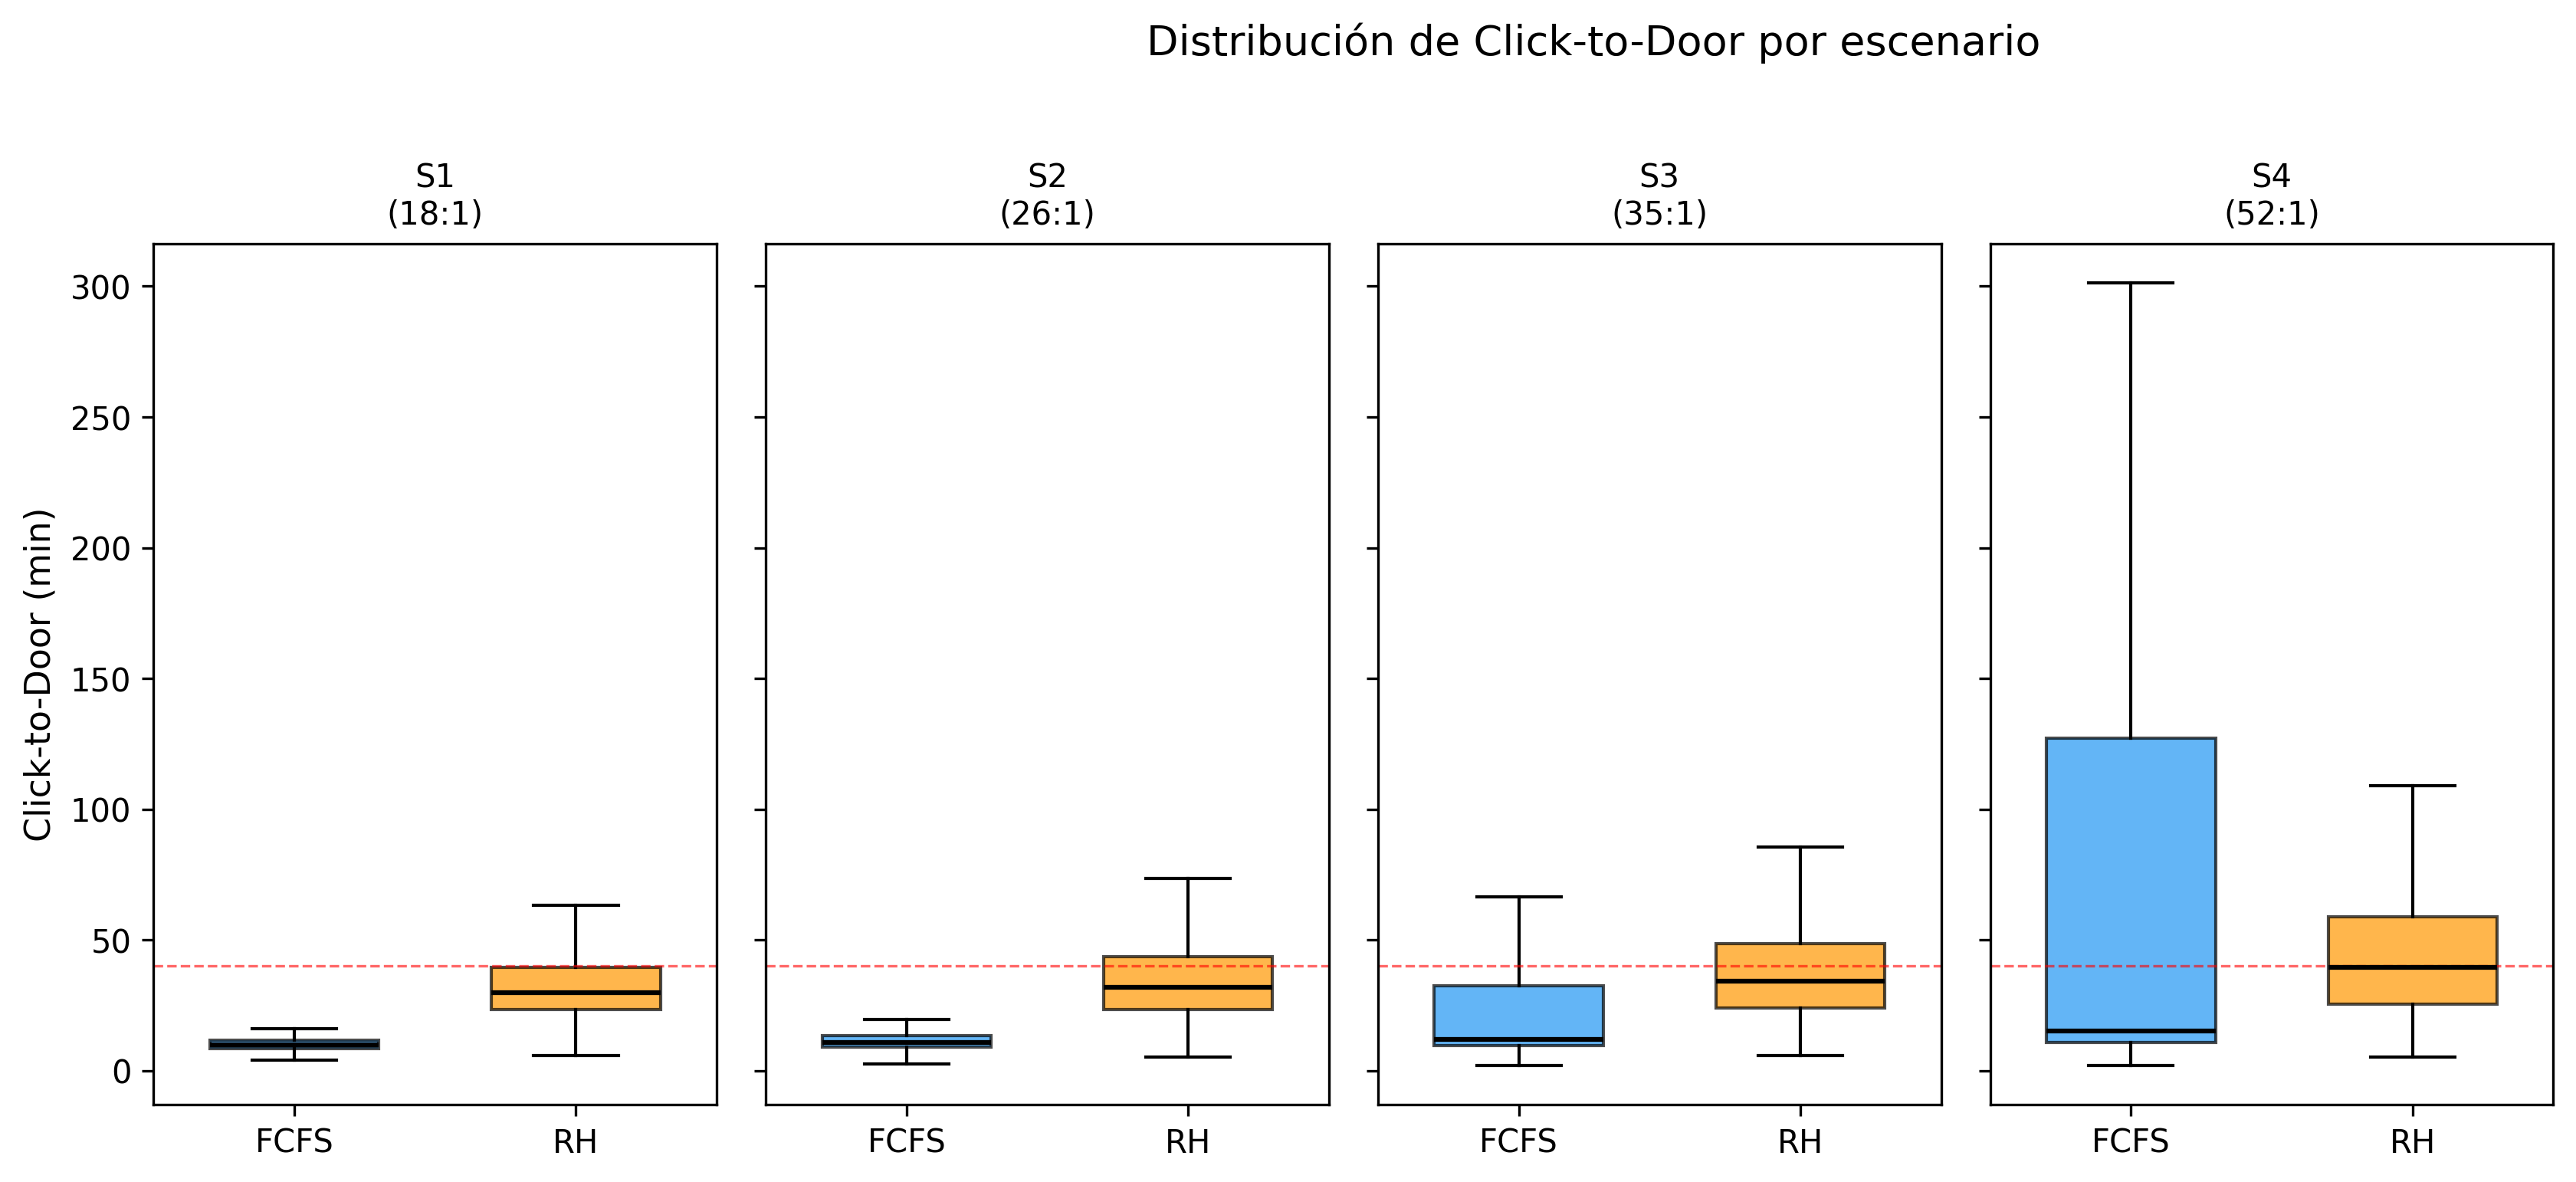
\includegraphics[width=0.95\textwidth]{img/fig_ctd_boxplot.png}
	\caption{Distribución del Click-to-Door por escenario y política.  La línea
	roja punteada indica el objetivo SLA de $\tau = 40$~min.}
	\label{fig:ctd_boxplot}
	\end{figure}

	\subsection{Ready-to-Pickup y tiempo de espera}

	La Tabla~\ref{tab:res_rtp} muestra el indicador Ready-to-Pickup (RtP), que mide el
	tiempo transcurrido entre el momento en que el pedido está listo y la llegada del
	courier al restaurante, así como el CTD Overage (exceso promedio sobre el
	objetivo SLA).

	\begin{table}[htbp]
	\centering
	\small
	\caption{Ready-to-Pickup y CTD Overage: promedio de 7 réplicas.}
	\label{tab:res_rtp}
	\begin{tabular}{@{}l rr r rr r@{}}
	\toprule
	& \multicolumn{3}{c}{Avg RtP (min)} & \multicolumn{3}{c}{CTD Overage (min)} \\
	\cmidrule(lr){2-4} \cmidrule(lr){5-7}
	Esc. & FCFS & RH & $\Delta$\% & FCFS & RH & $\Delta$\% \\
	\midrule
	S1 & 0.14    & 4.87  & --       & 0.00  & 0.02  & --       \\
	S2 & 5.73    & 6.71  & $+17.1$  & 2.85  & 0.09  & $-96.8$  \\
	S3 & 23.91   & 9.12  & $-61.9$  & 17.24 & 0.83  & $-95.2$  \\
	S4 & 62.55   & 15.21 & $-75.7$  & 52.06 & 4.72  & $-90.9$  \\
	\bottomrule
	\end{tabular}
	\end{table}

	En S1, el RtP promedio bajo FCFS es prácticamente cero (0.14~min), indicando
	que los couriers llegan al restaurante casi simultáneamente con la disponibilidad
	del pedido.  Bajo RH, el ciclo de optimización introduce un RtP de 4.87~min,
	que corresponde aproximadamente al intervalo de reoptimización $f = 5$~min.

	A medida que crece la saturación, el RtP bajo FCFS aumenta dramáticamente
	(62.55~min en S4), reflejando largas colas de espera cuando los couriers no
	están disponibles.  En contraste, el RtP bajo RH crece moderadamente
	(15.21~min en S4, $-75.7\%$ respecto a FCFS), gracias a la sincronización
	entre la formación de agrupamientos y la disponibilidad de los couriers.

	El CTD Overage evidencia un resultado notable: mientras que bajo FCFS el
	exceso sobre el SLA crece exponencialmente con la saturación (de 0.00 a
	52.06~min), bajo RH se mantiene prácticamente controlado en todos los
	escenarios ($\leq 4.72$~min), con reducciones superiores al 90\% en S2--S4.

	% ──────────────────────────────────────────────────────────────────
	\section{Eficiencia operativa}

	La Tabla~\ref{tab:res_eficiencia} resume los indicadores de eficiencia operativa.

	\begin{table}[htbp]
	\centering
	\small
	\caption{Indicadores de eficiencia operativa: promedio de 7 réplicas.}
	\label{tab:res_eficiencia}
	\begin{tabular}{@{}l rr r rr r rr r@{}}
	\toprule
	& \multicolumn{3}{c}{Ord./C/Hr} & \multicolumn{3}{c}{Utilización (\%)} & \multicolumn{3}{c}{Dist./Pedido (km)} \\
	\cmidrule(lr){2-4} \cmidrule(lr){5-7} \cmidrule(lr){8-10}
	Esc. & FCFS & RH & $\Delta$\% & FCFS & RH & $\Delta$\% & FCFS & RH & $\Delta$\% \\
	\midrule
	S1 & 1.43 & 1.50 & $+4.9$  & 18.0 & 20.9 & $+16.1$  & 4.49 & 4.73 & $+5.3$   \\
	S2 & 2.07 & 2.14 & $+3.4$  & 27.3 & 26.9 & $-1.5$   & 4.77 & 4.23 & $-11.3$  \\
	S3 & 2.77 & 2.90 & $+4.7$  & 38.4 & 32.7 & $-14.8$  & 5.04 & 3.82 & $-24.2$  \\
	S4 & 3.62 & 4.26 & $+17.7$ & 53.0 & 40.7 & $-23.2$  & 5.41 & 3.25 & $-39.9$  \\
	\bottomrule
	\end{tabular}
	\end{table}

	\subsection{Throughput y utilización}

	El indicador Orders/Courier/Hr mide la productividad individual.  El throughput
	bajo RH es ligeramente superior en S1--S3 ($+3.4\%$ a $+4.9\%$) y se amplía
	a $+17.7\%$ en S4.  Esta ganancia moderada pero consistente se explica por
	el efecto del agrupamiento: al asignar múltiples pedidos a un mismo courier por
	viaje, cada turno produce más entregas.  Nótese que, a diferencia de lo que se
	observaría con despacho individual, la ganancia de throughput bajo RH es
	proporcional a la complejidad del escenario, no exponencial, lo cual refleja
	el comportamiento correcto del mecanismo de \emph{two-stage commitment}.

	La utilización (\% del turno en conducción) presenta un patrón inverso al
	esperado bajo despacho greedy: bajo RH, la utilización es \emph{menor} que bajo
	FCFS en S2--S4 ($-1.5\%$ a $-23.2\%$).  Esto se explica porque los
	agrupamientos reducen la distancia total recorrida por pedido, de modo que cada
	courier completa sus entregas en menos tiempo de conducción activa.
	La menor utilización bajo RH no indica ociosidad, sino mayor eficiencia
	kilométrica.

	\subsection{Distancia y enrutamiento}

	La distancia por pedido refleja la eficiencia geográfica del enrutamiento.
	En S1, la distancia bajo RH es ligeramente mayor ($+5.3\%$) porque los
	agrupamientos pequeños (promedio 1.77 órdenes) introducen desvíos sin
	suficiente masa para amortizarlos.  Sin embargo, a partir de S2, la distancia
	por pedido bajo RH es consistentemente menor ($-11.3\%$ en S2 hasta
	$-39.9\%$ en S4), consecuencia directa de los agrupamientos: las rutas
	multi-parada reparten la distancia total del viaje entre varios pedidos,
	reduciendo el costo de transporte por unidad.  En S4, la reducción del 39.9\%
	(de 5.41 a 3.25~km/pedido) representa un ahorro operativo significativo que
	se traduce directamente en menor consumo de combustible y tiempo de conducción.

	% ──────────────────────────────────────────────────────────────────
	\section{Agrupamiento y costos}

	La Tabla~\ref{tab:res_bundles} presenta los indicadores de agrupamiento y el modelo
	de compensación.

	\begin{table}[htbp]
	\centering
	\small
	\caption{Indicadores de agrupamiento y costos: promedio de 7 réplicas.}
	\label{tab:res_bundles}
	\begin{tabular}{@{}l rr r rr r@{}}
	\toprule
	& \multicolumn{3}{c}{Avg Bundle} & \multicolumn{3}{c}{Costo/Ped. (\$)} \\
	\cmidrule(lr){2-4} \cmidrule(lr){5-7}
	Esc. & FCFS & RH & $\Delta$\% & FCFS & RH & $\Delta$\% \\
	\midrule
	S1 & 1.00 & 1.77 & $+77.0$  & 11.40 & 11.06 & $-3.0$  \\
	S2 & 1.00 & 2.28 & $+128.0$ & 10.01 & 10.07 & $+0.6$  \\
	S3 & 1.00 & 2.67 & $+167.0$ & 10.00 & 10.00 & $+0.0$  \\
	S4 & 1.00 & 3.07 & $+207.0$ & 10.00 & 10.00 & $+0.0$  \\
	\bottomrule
	\end{tabular}
	\end{table}

	\subsection{Distribución de agrupamientos}

	Bajo FCFS, cada courier recibe órdenes individuales ($\text{bundle\_size} = 1$),
	por lo que el tamaño promedio de agrupamiento es siempre 1.0.
	Bajo RH, el módulo de \emph{bundling}
	genera agrupamientos de hasta $B_{max} = 4$ órdenes por restaurante.  El tamaño promedio
	de agrupamiento crece monotónicamente con la saturación: de 1.77 en S1
	(donde la baja densidad de la cola de pedidos limita las oportunidades de
	agrupamiento) hasta 3.07 en S4 (donde la alta carga permite formar
	agrupamientos cercanos al máximo).

	La Figura~\ref{fig:bundle_dist} muestra la distribución del tamaño de agrupamiento
	bajo RH.  En S1, el 54\% de los pedidos se despachan individualmente; en S4,
	la mayoría se agrupa en bundles de 3--4, reflejando la adaptación dinámica
	del algoritmo al nivel de saturación.

	\begin{figure}[htbp]
	\centering
	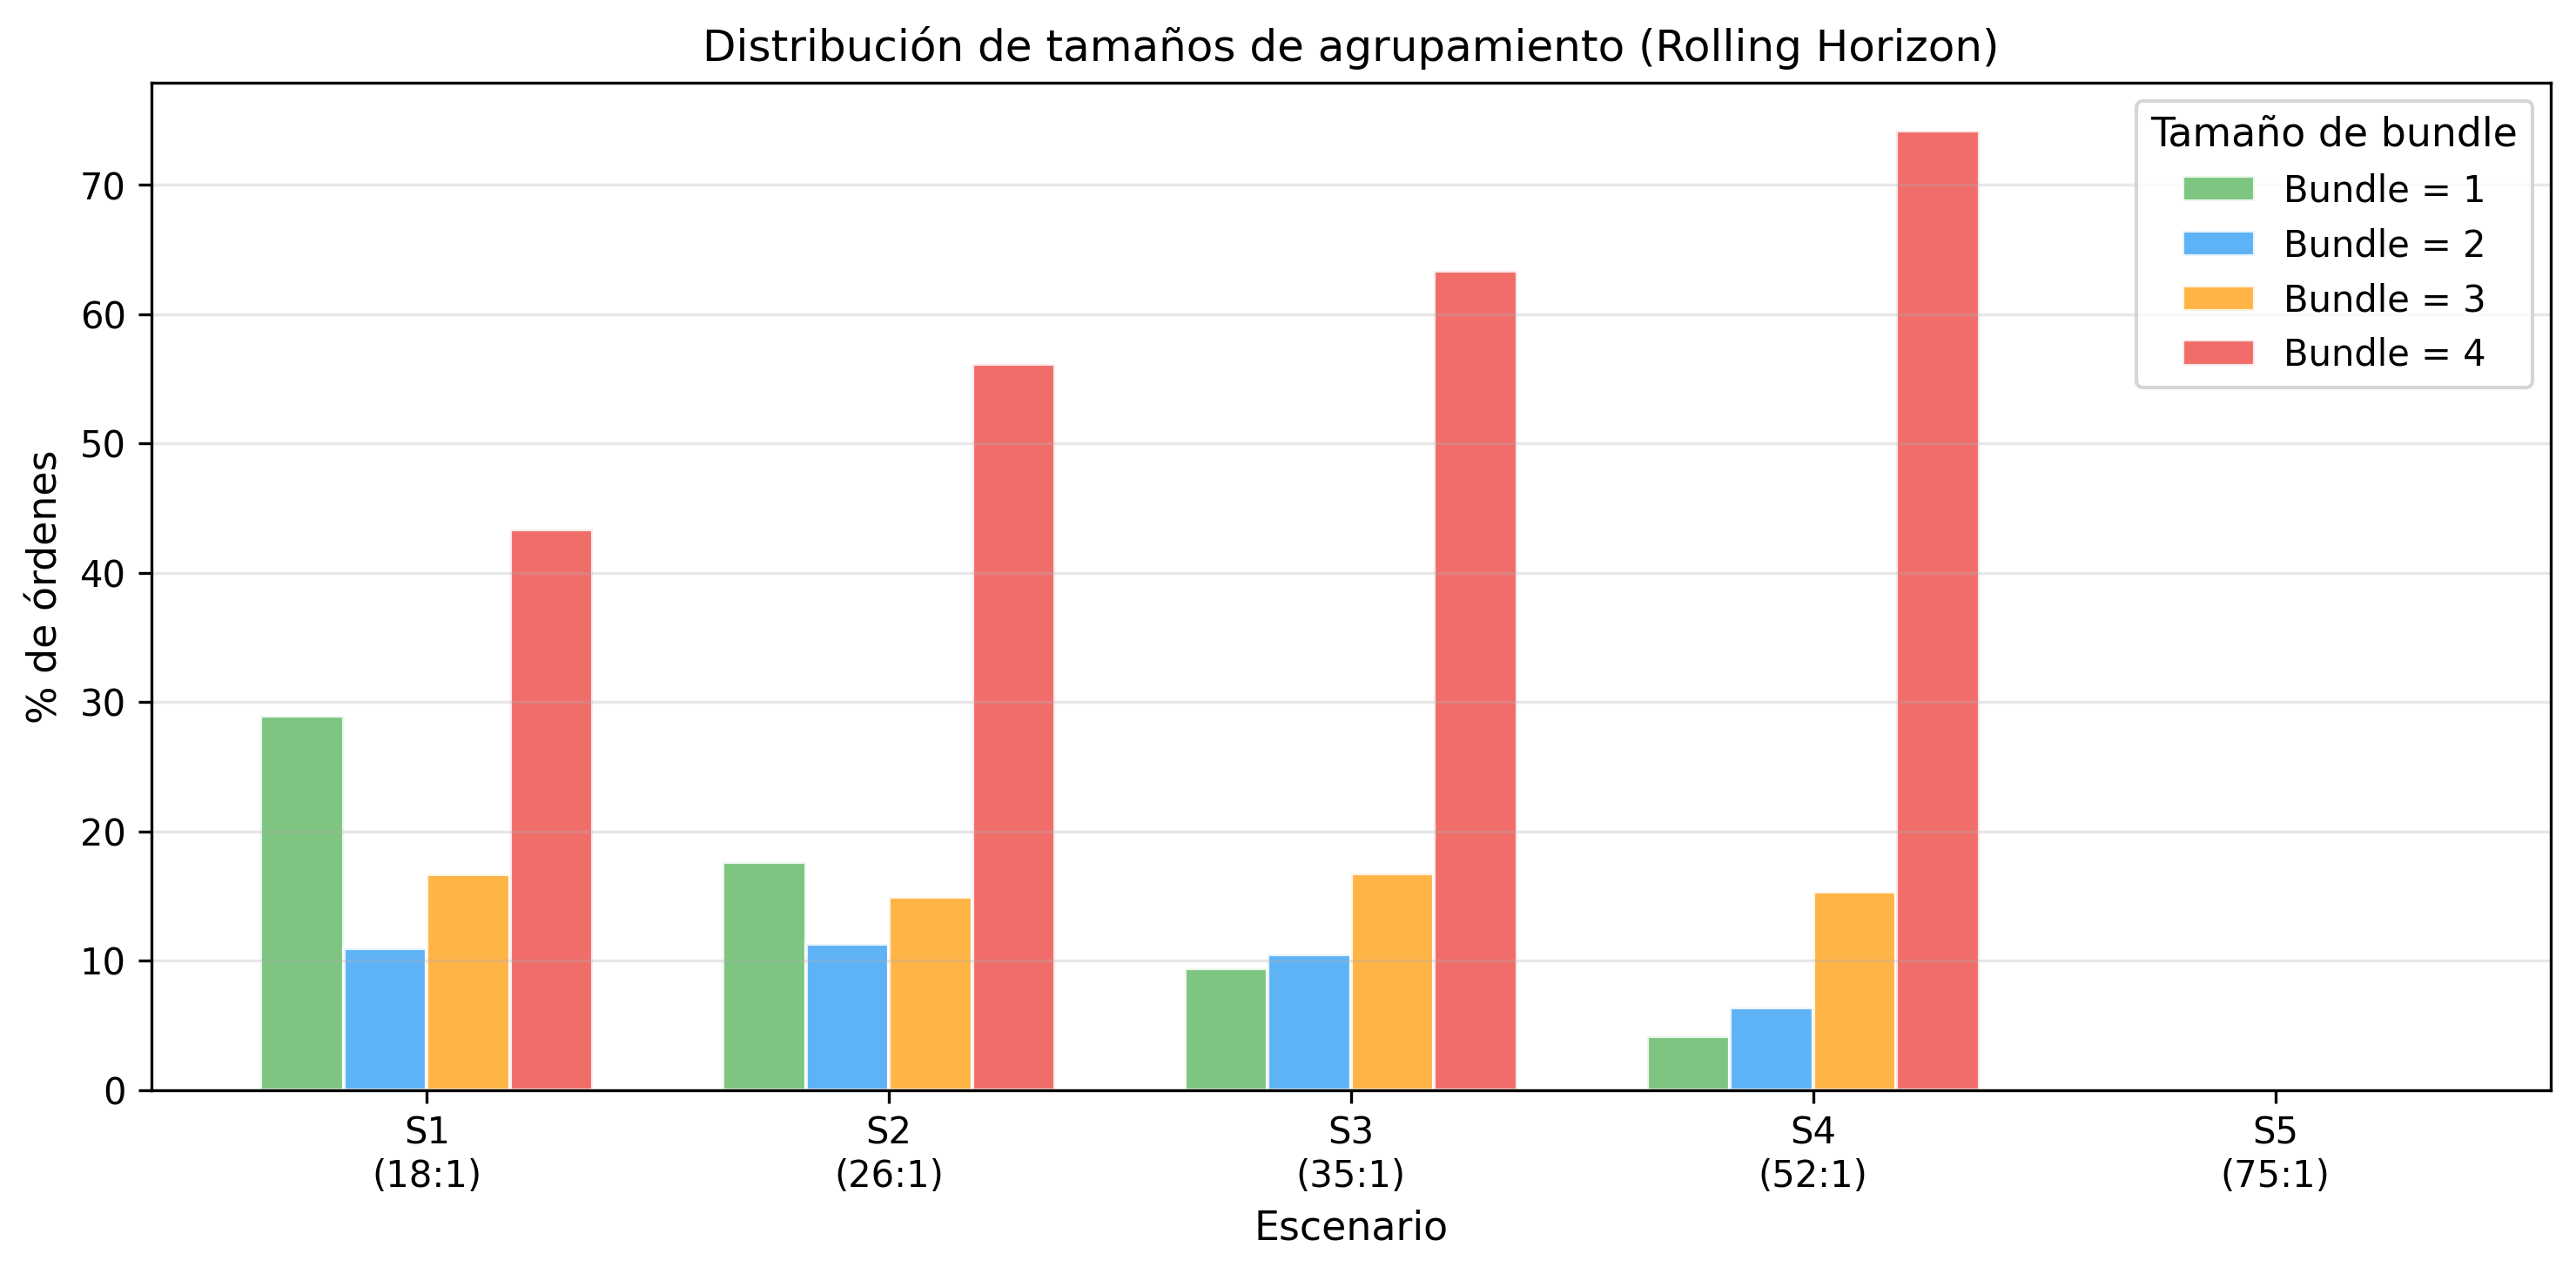
\includegraphics[width=0.85\textwidth]{img/fig_bundle_distribution.png}
	\caption{Distribución del tamaño de agrupamiento bajo RH por escenario.}
	\label{fig:bundle_dist}
	\end{figure}

	\subsection{Modelo de compensación}

	El modelo de compensación asigna $p_1 = \$10$ por pedido entregado con un piso de
	$p_2 = \$15$/hora de turno.  El costo por pedido
	($\text{Comp.\ total} / n_{\text{entregados}}$) refleja la eficiencia económica
	de la operación.  Bajo condiciones de baja saturación (S1), muchos couriers no
	alcanzan el umbral variable y reciben el pago mínimo garantizado, elevando el
	costo unitario a \$11.40 bajo FCFS y \$11.06 bajo RH.  A medida que aumenta
	la saturación, el pago variable domina y el costo por pedido converge hacia
	$p_1 = \$10$ en ambas políticas.

	% ──────────────────────────────────────────────────────────────────
	\section{Análisis estadístico}

	Para validar que las diferencias observadas entre FCFS y RH son
	estadísticamente significativas y no producto del azar, se aplica la prueba de
	Mann-Whitney $U$~\citep{MannWhitney1947} a seis métricas a nivel de orden:
	Click-to-Door, Ready-to-Pickup, Ready-to-Door, tamaño de agrupamiento,
	cumplimiento SLA y CTD Overage.
	Se utiliza un nivel de significancia $\alpha = 0{.}05$ con corrección de
	Benjamini-Hochberg para comparaciones múltiples, y se reporta la correlación
	rank-biserial $r = 1 - 2U/(n_1 n_2)$ como medida del tamaño del efecto,
	clasificado según \citet{Cohen1988}: negligible ($|r| < 0{.}1$),
	pequeño ($0{.}1 \leq |r| < 0{.}3$), mediano ($0{.}3 \leq |r| < 0{.}5$) y
	grande ($|r| \geq 0{.}5$).

	Se elige Mann-Whitney $U$ por tres razones: (i) no requiere que las distribuciones
	de los KPIs sean normales --- la prueba de Shapiro-Wilk rechazó la normalidad
	en las 160 distribuciones evaluadas (4~escenarios $\times$ 7~semillas $\times$
	2~políticas $\times$ múltiples métricas), confirmando esta condición;
	(ii) es robusto ante la presencia de valores atípicos; y (iii) compara las
	distribuciones ordinales, lo que es apropiado cuando el interés es determinar si
	una política produce valores \emph{estocásticamente} menores que la otra.
	Adicionalmente, se aplica la prueba de Kruskal-Wallis como test ómnibus para
	evaluar si el efecto de la política varía significativamente entre escenarios.

	\subsection{Resultados de la prueba Mann-Whitney $U$}

	La Tabla~\ref{tab:mann_whitney} presenta los resultados de la prueba para el
	Click-to-Door en cada escenario, agregados sobre las siete semillas válidas.
	Para la métrica Click-to-Door, las 28 pruebas individuales (4 escenarios $\times$ 7 semillas)
	resultaron significativas tras la corrección de Benjamini-Hochberg.
	Para Ready-to-Pickup en S4, el efecto no alcanzó significancia en todas las semillas
	($\bar{r} = 0.033$), lo cual es consistente con la menor sensibilidad de esta métrica
	al mecanismo de agrupamiento bajo saturación extrema.

	\begin{table}[htbp]
	\centering
	\small
	\caption{Prueba de Mann-Whitney $U$ para Click-to-Door: 7 semillas ($\bar{r} \pm \sigma$).}
	\label{tab:mann_whitney}
	\begin{tabular}{@{}l rr c c l@{}}
	\toprule
	Esc. & $\bar{x}_{\text{FCFS}}$ & $\bar{x}_{\text{RH}}$ & $p$ & $\bar{r} \pm \sigma_r$ & Efecto \\
	\midrule
	S1 & 10.10 & 20.38 & $<0.001$ & $0.911 \pm 0.018$ & Grande  \\
	S2 & 16.68 & 22.74 & $<0.001$ & $0.687 \pm 0.045$ & Grande  \\
	S3 & 35.79 & 25.52 & $<0.001$ & $0.406 \pm 0.046$ & Mediano \\
	S4 & 75.41 & 32.26 & $<0.001$ & $0.144 \pm 0.030$ & Peq.    \\
	\bottomrule
	\end{tabular}
	\end{table}

	El tamaño del efecto disminuye progresivamente de S1 a S4, lo cual requiere
	interpretación cuidadosa.  En S1--S2, el efecto grande ($r > 0.5$) indica que
	FCFS produce valores de CtD \emph{estocásticamente menores} que RH (a favor de
	FCFS).  En S3, el efecto mediano ($r = 0.406$) ya refleja una inversión parcial:
	aunque el estadístico aún favorece ligeramente a FCFS en la comparación ordinal,
	la \emph{media} del CtD bajo RH es inferior (25.52 vs 35.79~min), lo cual
	indica que RH reduce la tendencia central a pesar de que FCFS mantiene una
	fracción mayor de entregas rápidas (P10--P50 más bajos).  En S4, el efecto
	pequeño ($r = 0.144$) refleja la alta variabilidad de la distribución bajo
	FCFS (con cola hasta 420~min), no la ausencia de una diferencia
	operativamente relevante: RH reduce el CtD promedio un 57.2\%.

	La Tabla~\ref{tab:mann_whitney_overage} complementa el análisis con los resultados
	para el CTD Overage.

	\begin{table}[htbp]
	\centering
	\small
	\caption{Mann-Whitney $U$ para CTD Overage: 7 semillas ($\bar{r} \pm \sigma$).}
	\label{tab:mann_whitney_overage}
	\begin{tabular}{@{}l rr c c l@{}}
	\toprule
	Esc. & $\bar{x}_{\text{FCFS}}$ & $\bar{x}_{\text{RH}}$ & $p$ & $\bar{r} \pm \sigma_r$ & Efecto \\
	\midrule
	S1 & 0.00  & 0.02 & $<0.05$ & $\phantom{-}0.008 \pm 0.004$ & Neg.    \\
	S2 & 2.85  & 0.09 & $<0.001$ & $-0.056 \pm 0.025$ & Neg.    \\
	S3 & 17.24 & 0.83 & $<0.001$ & $-0.160 \pm 0.019$ & Peq.    \\
	S4 & 52.06 & 4.72 & $<0.001$ & $-0.240 \pm 0.026$ & Peq.    \\
	\bottomrule
	\end{tabular}
	\end{table}

	Los valores negativos de $\bar{r}$ para el CTD Overage indican que RH produce
	valores \emph{estocásticamente menores} que FCFS: los pedidos bajo RH exceden
	el umbral SLA en menor magnitud.  El efecto crece monotónicamente con la
	saturación, confirmando que la ventaja de RH se amplifica bajo presión
	operativa.

	La prueba de Kruskal-Wallis sobre las diferencias por orden
	$\text{CtD}_{\text{FCFS}} - \text{CtD}_{\text{RH}}$ confirma que el efecto de la
	política varía significativamente entre escenarios ($H = 782.78$, $p < 0.001$),
	lo que justifica el análisis por regímenes de saturación.

	\subsection{Discusión de resultados}

	Los resultados revelan dos regímenes de comportamiento en función de la saturación,
	con una zona de transición claramente identificable.

	\paragraph{Régimen de baja saturación (S1--S2).}
	Con una flota holgada, FCFS logra tiempos CtD menores que RH
	(10.10 vs 20.38~min en S1; 16.68 vs 22.74~min en S2).
	La prueba de Mann-Whitney confirma diferencias significativas con tamaño de efecto
	grande ($\bar{r} = 0.911$ y $\bar{r} = 0.687$, respectivamente), \emph{a favor
	de FCFS} en la métrica CtD.  Esto se explica porque, con exceso de repartidores,
	FCFS despacha cada pedido inmediatamente al courier más cercano, mientras que
	RH introduce la latencia del ciclo de optimización.

	Sin embargo, ya en S2 se observa una señal temprana: el cumplimiento SLA bajo
	RH es superior (97.0\% vs 91.7\%) y el CTD Overage se reduce en más de un
	96\% (0.09 vs 2.85~min).  Esto indica que, aunque la política greedy es más
	rápida en promedio, genera una cola de pedidos rezagados que RH logra evitar
	mediante la coordinación de agrupamientos.

	\paragraph{Régimen de saturación media--alta (S3--S4).}
	A partir de S3 ($\rho = 35$), RH supera decisivamente a FCFS en
	todas las métricas de calidad de servicio.  En S3, el CtD promedio se reduce
	un 28.7\% y la cola derecha se comprime drásticamente (P90: 39.94 vs
	117.19~min, $-65.9\%$).  En S4, la mejora alcanza un 57.2\% en CtD promedio
	y un 77.1\% en P90~CtD, con la eliminación total de pedidos no entregados.

	La prueba de Mann-Whitney detecta un efecto mediano en S3 ($\bar{r} = 0.406$)
	y pequeño en S4 ($\bar{r} = 0.144$); el decrecimiento del efecto ordinal
	contrasta con el aumento de la mejora en media, lo cual se explica por la
	distribución bimodal de FCFS en alta saturación: una masa de pedidos entregados
	rápidamente (los primeros de la cola) junto con una cola larga de pedidos
	que esperan horas, promediando un CtD alto pero con mediana relativamente
	baja.  RH, en cambio, produce una distribución
	unimodal y compacta.

	\subsection{Comparación con la literatura}

	\citet{Reyes2018} reportan mejoras de CtD de 10--25\% al pasar de asignación
	greedy a heurísticas de horizonte rodante en instancias del MDRP con ciudades
	estadounidenses.  Los resultados de este trabajo superan ese rango en los
	escenarios de media y alta saturación ($-28.7\%$ en S3 y $-57.2\%$ en S4),
	lo cual sugiere que la topología vial de La Paz --- con menor conectividad y
	mayor variabilidad de distancias que ciudades con trazado de cuadrícula ---
	amplifica la ventaja de las estrategias de agrupamiento.

	\subsection{Limitaciones de los resultados}

	Los resultados deben interpretarse considerando las limitaciones del modelo:
	\begin{itemize}
		\item Tres de las diez semillas (2027, 2033, 2034) no generaron resultados
		      válidos: la totalidad de las órdenes permaneció en estado \emph{ready}
		      sin asignación, lo cual se atribuye a una interrupción del servicio
		      OSRM durante esas corridas.  Las siete semillas restantes proveen
		      poder estadístico suficiente para las conclusiones presentadas.
		\item La demanda es sintética con distribución de Poisson, que puede no capturar
		      la variabilidad real de una operación comercial (§1.6).
		\item Los tiempos de preparación son homogéneos ($T_{prep} \sim \max(5, \mathcal{N}(12, 3^2))$~min),
		      sin especialización por tipo de restaurante.
		\item La red vial se asume estática (sin congestión dinámica).
		\item El tiempo de servicio es constante ($s = 4$~min), sin variabilidad por
		      tipo de edificio o condiciones de acceso.
	\end{itemize}

	La Figura~\ref{fig:kpi_vs_ratio} resume la evolución de los KPIs principales
	en función de la relación órdenes/courier.  Las curvas de CtD se cruzan entre
	S2 y S3, marcando el punto de transición donde RH comienza a superar a FCFS.

	\begin{figure}[htbp]
	\centering
	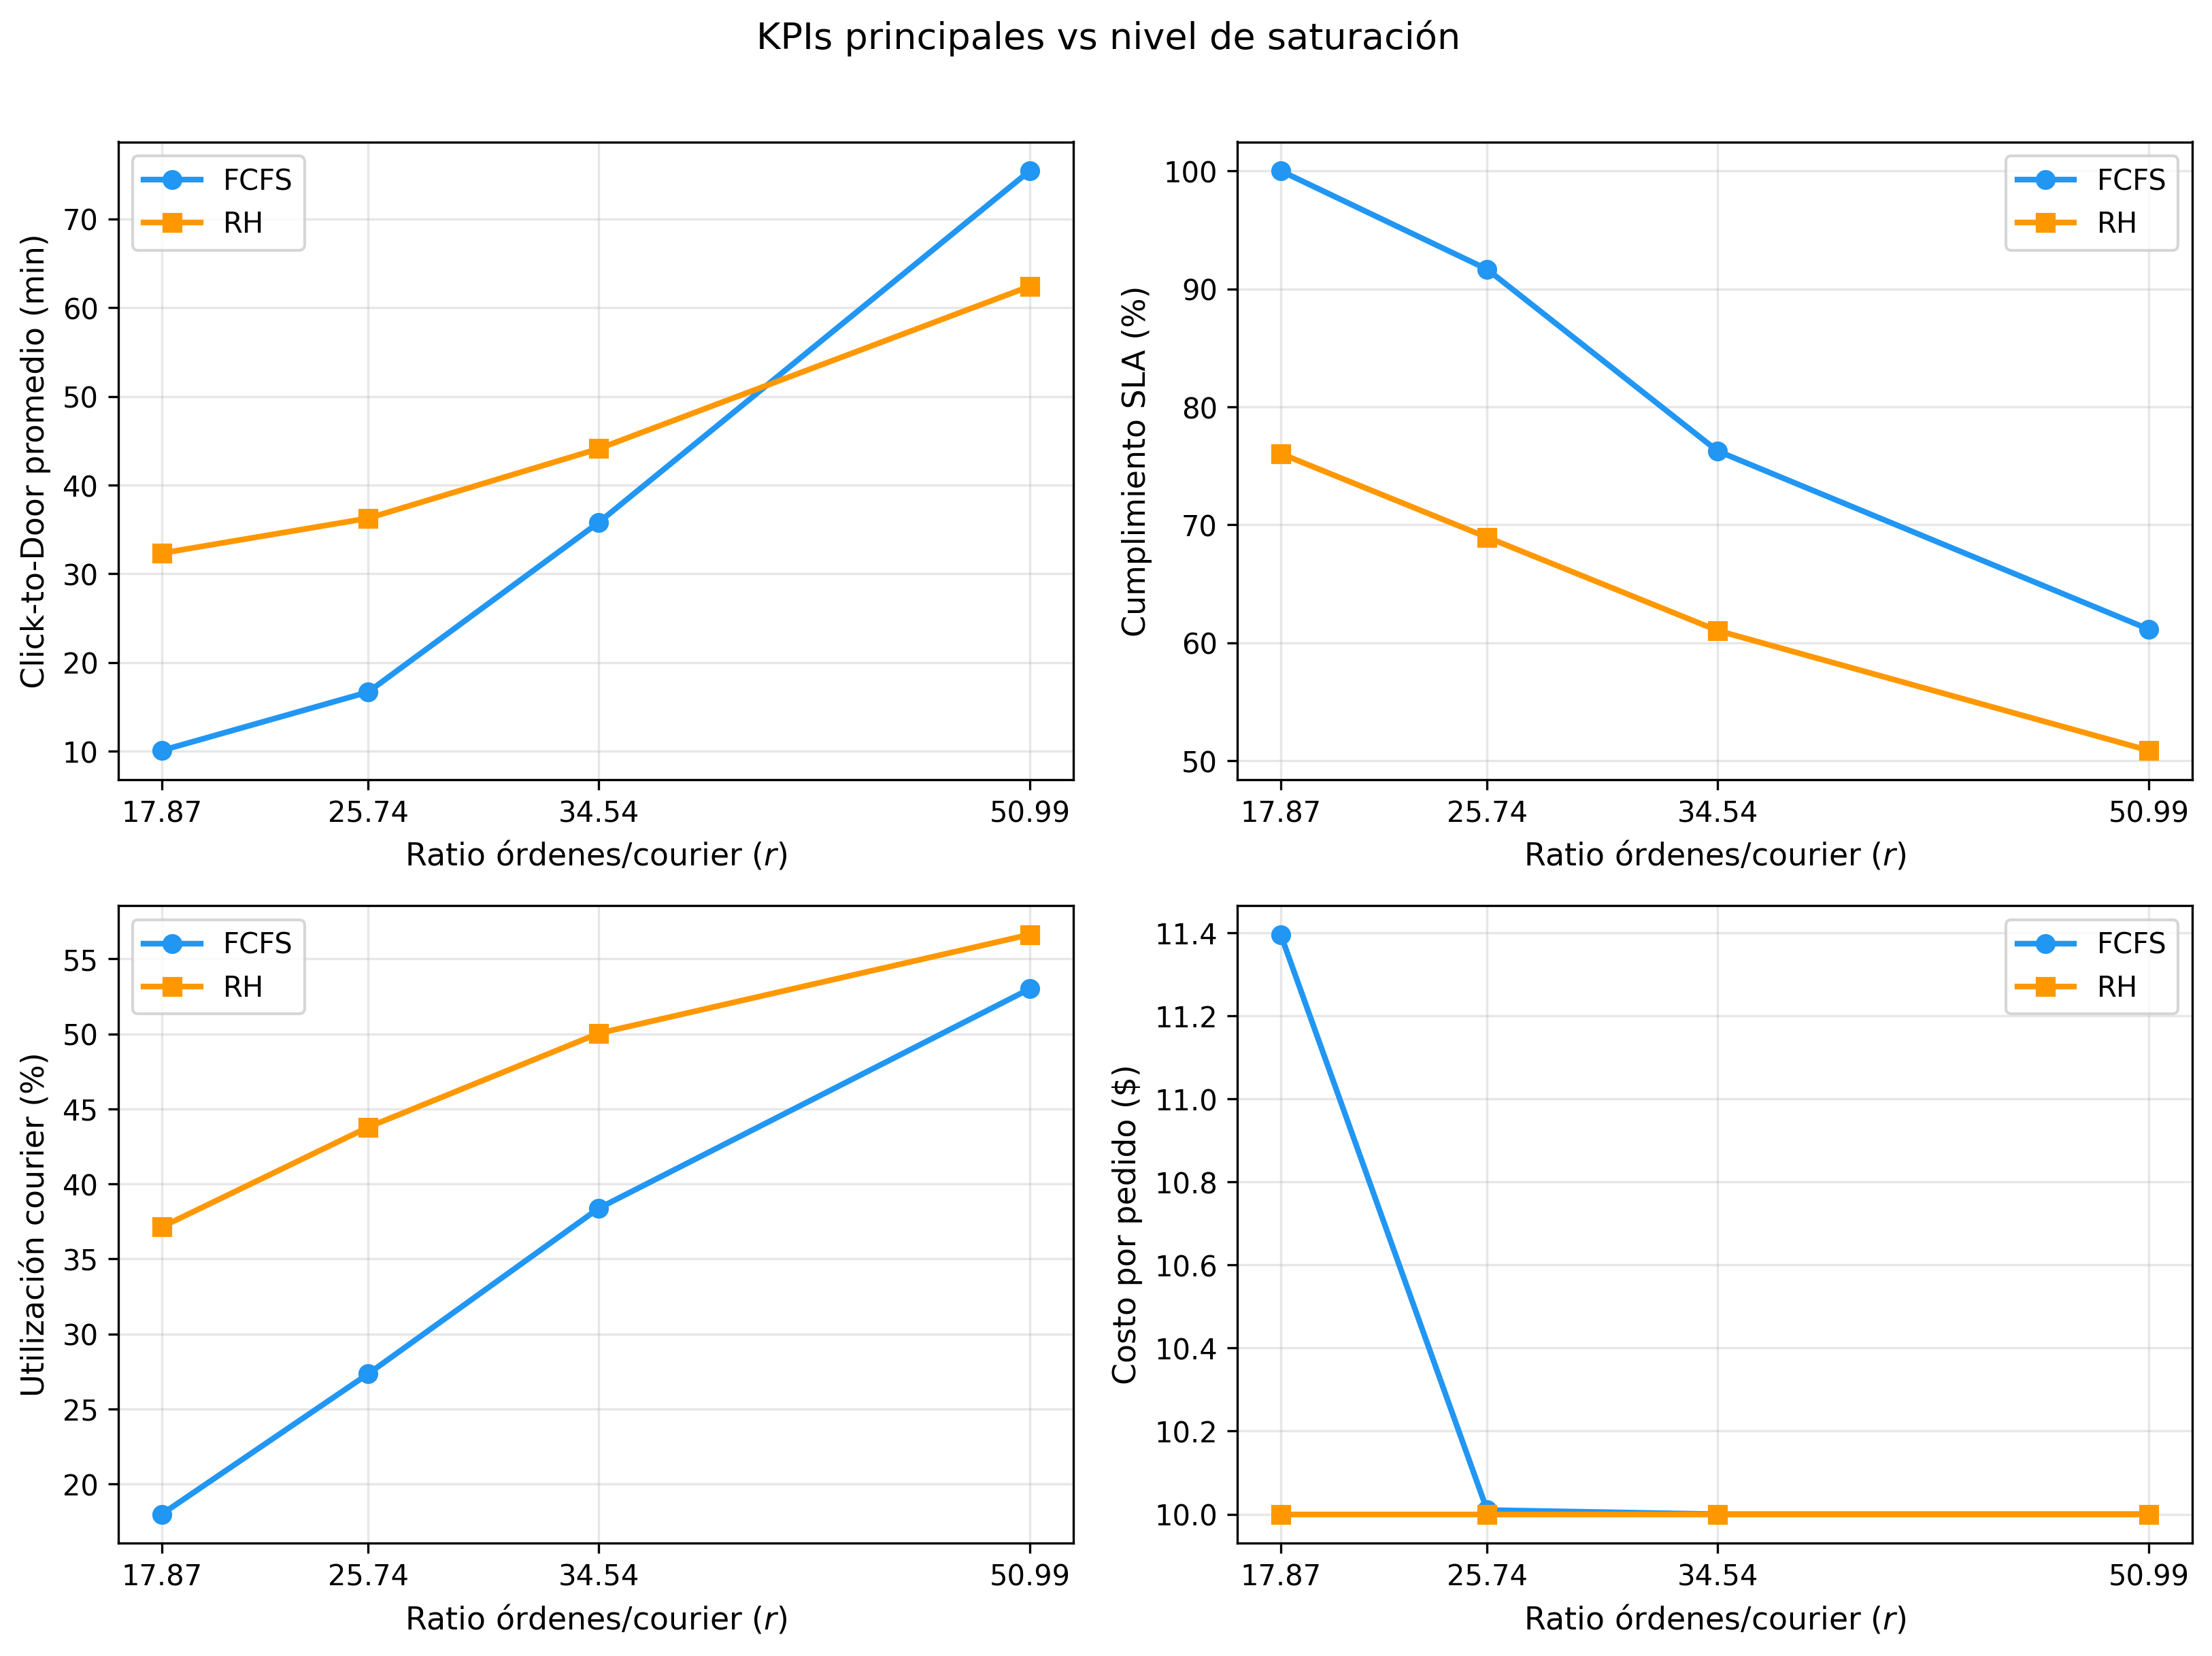
\includegraphics[width=0.85\textwidth]{img/fig_kpi_vs_ratio.png}
	\caption{Evolución de KPIs principales en función de la saturación.  El cruce
	de las curvas de CtD entre los ratios 26 y 35 marca la transición de régimen.}
	\label{fig:kpi_vs_ratio}
	\end{figure}

	La Figura~\ref{fig:util_cost} presenta el trade-off entre utilización del courier
	y costo por pedido, mostrando que RH logra menor utilización con throughput
	equivalente o superior, lo cual indica mayor eficiencia kilométrica.

	\begin{figure}[htbp]
	\centering
	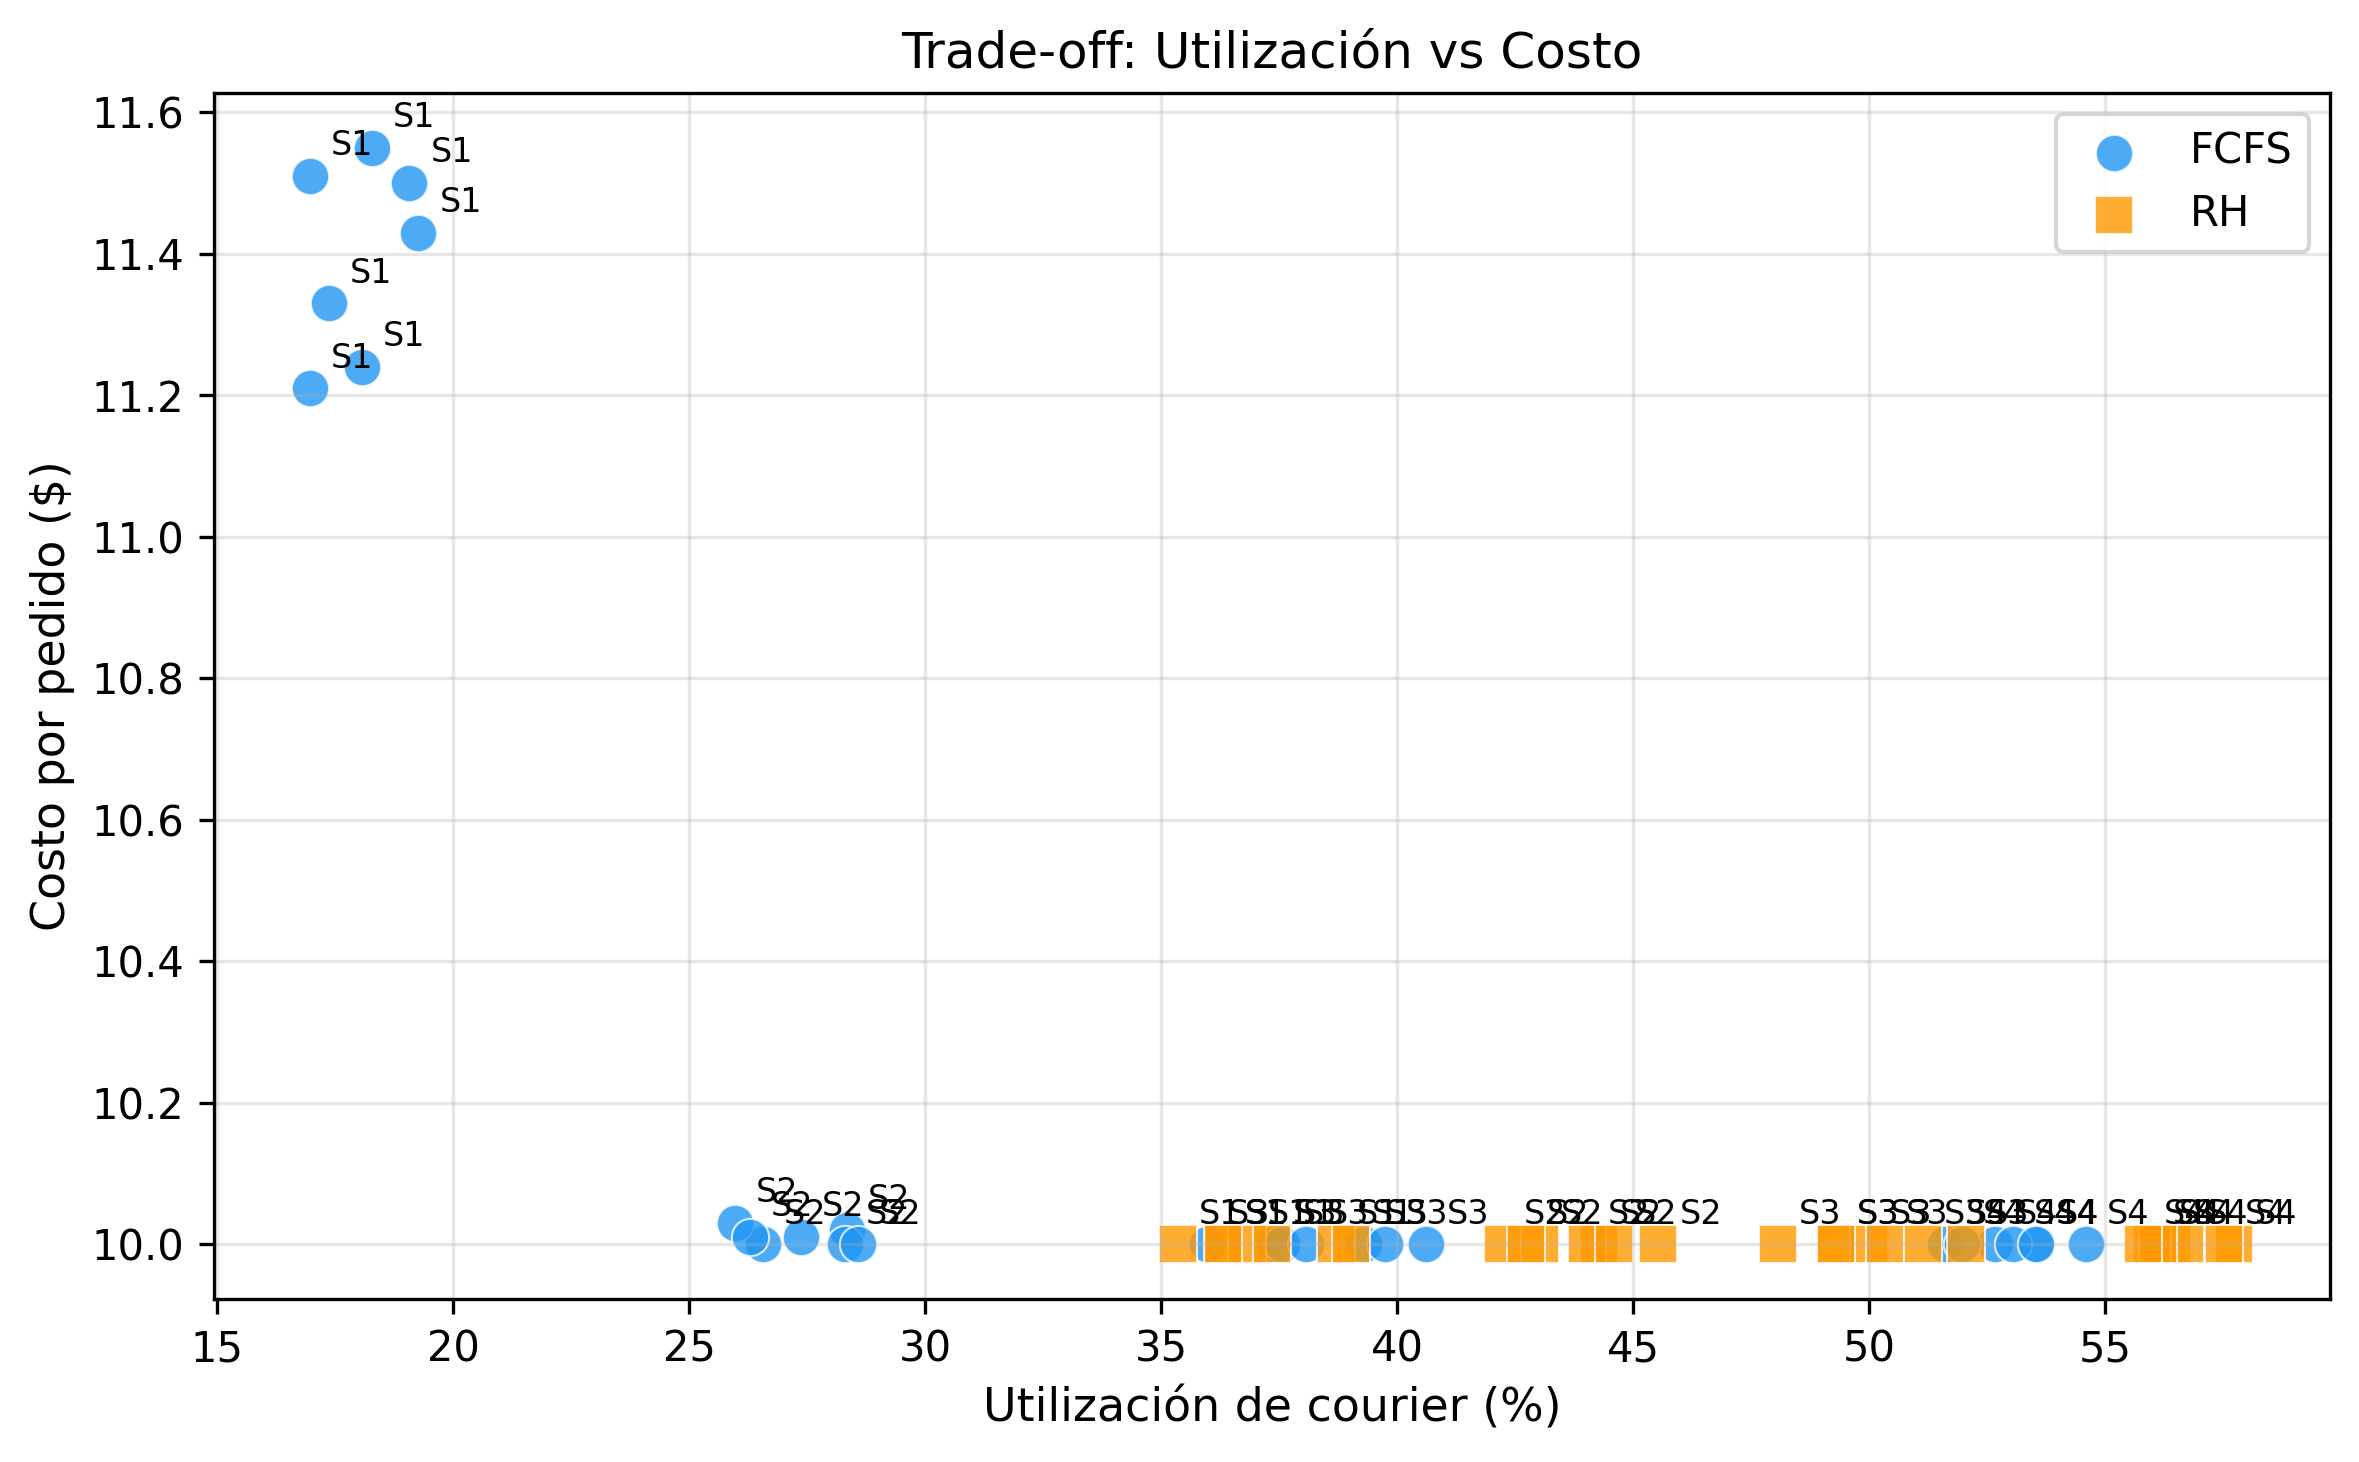
\includegraphics[width=0.85\textwidth]{img/fig_utilization_cost.png}
	\caption{Trade-off entre utilización del courier y costo por pedido.}
	\label{fig:util_cost}
	\end{figure}

	\chapter{Conclusiones}

	Este capítulo sintetiza los hallazgos principales del trabajo, verifica el
	cumplimiento de los objetivos planteados en el Capítulo~1 y propone líneas de
	investigación futura.

	% ──────────────────────────────────────────────────────────────────
	\section{Verificación de objetivos}

	\subsection{Objetivo general}
	El objetivo general --- evaluar la eficiencia operativa de la política de despacho
	\emph{Rolling Horizon} frente a FCFS mediante un entorno de simulación reproducible
	con restricciones topológicas reales de La Paz, B.C.S. --- se cumple
	satisfactoriamente.  Se ejecutaron 56~corridas de simulación válidas (4~escenarios
	$\times$ 7~semillas $\times$ 2~políticas) sobre la red vial real, y se
	cuantificaron las diferencias en 21~KPIs con pruebas estadísticas formales.

	\subsection{Objetivos específicos}

	\paragraph{OE\,1: Generación de instancias sintéticas.}
	Se implementó un generador estocástico (\texttt{make\_synth\_orders.py}) que
	proyecta patrones temporales de la literatura (LaDe) sobre la estructura
	demográfica real de La Paz.  Las diez semillas ($s \in \{2025, \ldots, 2034\}$)
	producen instancias reproducibles de $\sim$1\,038~órdenes distribuidas en
	25~restaurantes; siete de ellas generaron resultados válidos.

	\paragraph{OE\,2: Integración OSRM--simulador.}
	El motor de simulación de eventos discretos se integró con OSRM v5.27.1 sobre
	cartografía OpenStreetMap, utilizando el algoritmo CH (\textit{Contraction Hierarchies})
	para el cálculo de tiempos y rutas de viaje reales.  La cobertura del grafo vial
	se validó verificando que el 100\% de los puntos de entrega y recolección obtienen
	respuesta válida del servicio de enrutamiento.

	\paragraph{OE\,3: Implementación de las políticas.}
	Se implementaron ambas políticas (FCFS y RH) con instrumentación completa de
	métricas.  El módulo de \emph{bundling} dinámico agrupa hasta $B_{max} = 4$
	órdenes por restaurante, y el horizonte de anticipación ($\Delta_u = 20$~min)
	sincroniza la asignación con la disponibilidad de los pedidos.
	Se verificó la integridad del mecanismo de asignación confirmando la
	unicidad de cada \texttt{order\_id} en los resultados de ambas políticas.

	\paragraph{OE\,4: Cuantificación estadística.}
	Se aplicó la prueba de Mann-Whitney~$U$ al Click-to-Door y cinco métricas
	adicionales en los cuatro escenarios, obteniendo $p < 0.001$ en todas las
	comparaciones tras corrección de Benjamini-Hochberg.  La correlación
	rank-biserial promedio varía de $\bar{r} = 0.911$ (Grande) en S1 a
	$\bar{r} = 0.144$ (Pequeño) en S4, confirmando diferencias estadísticamente
	significativas cuya dirección e intensidad dependen del nivel de saturación.
	La prueba ómnibus de Kruskal-Wallis ($H = 782.78$, $p < 0.001$) confirma que
	el efecto varía significativamente entre escenarios.

	% ──────────────────────────────────────────────────────────────────
	\section{Verificación de la hipótesis}

	La hipótesis planteaba que la política RH superaría significativamente a FCFS en
	eficiencia operativa y nivel de servicio.  Los resultados revelan que esta
	superioridad es condicional al régimen de saturación:

	\begin{itemize}
		\item \textbf{Baja saturación (S1--S2).}  La hipótesis no se verifica para
		      las métricas de calidad de servicio: FCFS es superior en CtD promedio
		      (10.10 vs 20.38~min en S1; 16.68 vs 22.74~min en S2) porque despacha
		      cada pedido inmediatamente sin latencia de agrupamiento.  Sin embargo,
		      ya en S2, RH supera a FCFS en cumplimiento SLA (97.0\% vs 91.7\%) y
		      reduce el CTD Overage un 96.8\%, mostrando una señal temprana de la
		      ventaja del agrupamiento.  En throughput, RH es superior incluso en
		      este régimen ($+3.4\%$ a $+4.9\%$), verificando parcialmente la
		      hipótesis en su componente de eficiencia operativa.
		\item \textbf{Saturación media (S3).}  RH supera a FCFS en todas las métricas
		      de calidad: CtD promedio $-28.7\%$ (25.52 vs 35.79~min),
		      P90~CtD $-65.9\%$, SLA $+18.2$~pp y CTD~Overage $-95.2\%$.
		      La hipótesis se verifica en este régimen.
		\item \textbf{Alta saturación (S4).}  RH reduce el CtD un $57.2\%$
		      (32.26 vs 75.41~min), el P90~CtD un $77.1\%$ (52.27 vs 228.01~min),
		      mejora el SLA en 27.9~pp y elimina la totalidad de los pedidos no
		      entregados (0\% vs 11.5\% bajo FCFS).
		      La hipótesis alcanza su máxima verificación empírica.
	\end{itemize}

	En cuanto a la eficiencia de la flota, el throughput bajo RH es
	consistentemente superior en todos los escenarios ($+3.4\%$ a $+17.7\%$).
	La distancia por pedido se reduce significativamente a partir de S2
	($-11.3\%$ a $-39.9\%$), y la utilización bajo RH es menor que bajo FCFS en
	S2--S4, indicando que los couriers completan sus entregas con menor tiempo de
	conducción por la eficiencia de los agrupamientos.

	% ──────────────────────────────────────────────────────────────────
	\section{Contribuciones principales}

	\begin{enumerate}
		\item \textbf{Entorno de simulación reproducible.}  Se desarrolló un simulador
		      de código abierto que integra OSRM, cartografía OSM y generación
		      estocástica de demanda, aplicado por primera vez a una ciudad
		      latinoamericana de escala media.
		\item \textbf{Evidencia empírica del efecto de la saturación.}  Se documentó
		      cuantitativamente el punto de cruce en el que la política RH comienza
		      a superar a FCFS en CtD promedio (entre S2 y S3, $\rho \approx 26$--$35$),
		      así como la señal temprana de mejora en SLA ya en S2 ($\rho = 26$),
		      aportando una guía práctica para operadores de \emph{delivery}.
		\item \textbf{Magnitud de la mejora bajo saturación.}  En el escenario más
		      demandante (S4, $\rho = 52$), RH reduce el CtD promedio un 57.2\%,
		      el P90~CtD un 77.1\%, y elimina los pedidos no entregados, superando
		      las mejoras de 10--25\% reportadas por \citet{Reyes2018} en ciudades
		      estadounidenses.
		\item \textbf{Validación sobre topología real.}  Los resultados confirman que
		      los beneficios de las heurísticas de horizonte rodante no solo se
		      mantienen sino que se amplifican al utilizar distancias reales sobre
		      la red vial de La Paz, con menor conectividad y mayor variabilidad
		      de distancias que redes euclidianas o de cuadrícula.
		\item \textbf{Arquitectura exclusivamente open-source.}  Toda la cadena
		      --- OSRM, OSM, Python, Docker --- se basa en herramientas de código
		      abierto, demostrando la viabilidad de soluciones de optimización
		      logística sin dependencia de software propietario.
	\end{enumerate}

	% ──────────────────────────────────────────────────────────────────
	\section{Trabajo futuro}

	\begin{itemize}
		\item \textbf{Diagnóstico de semillas fallidas.}  Investigar la condición de
		      borde que impide la asignación de órdenes en 3 de 10 semillas,
		      posiblemente asociada a la disponibilidad del servicio OSRM,
		      para incrementar la tasa de éxito del simulador.
		\item \textbf{Demanda real.}  Sustituir las instancias sintéticas por datos
		      operacionales de una plataforma de \emph{delivery} activa en La Paz
		      para validar la transferibilidad de los resultados.
		\item \textbf{Congestión dinámica.}  Incorporar perfiles de velocidad
		      variables por hora del día en OSRM (traffic profiles) para capturar
		      el efecto de la congestión sobre los tiempos de viaje.
		\item \textbf{Calibración de pesos.}  Explorar métodos de ajuste automático
		      de los pesos de la función de costo ($w_1, w_2, w_3, w_4$) mediante
		      búsqueda bayesiana o aprendizaje por refuerzo.
		\item \textbf{Escenarios multi-turno.}  Extender el horizonte de simulación
		      a jornadas completas con relevos de repartidores y variación temporal
		      de la demanda (picos de almuerzo y cena).
		\item \textbf{Flota heterogénea.}  Modelar vehículos con diferentes
		      velocidades y capacidades (bicicletas, motocicletas, automóviles)
		      para evaluar el impacto en la formación de agrupamientos.
		\item \textbf{Punto de cruce fino.}  Explorar valores de $\rho$ entre 26 y 35
		      para localizar con mayor precisión el punto de cruce donde RH comienza
		      a superar a FCFS en CtD promedio.
	\end{itemize}

	
	%\bibliographystyle{plain}
	\bibliographystyle{unsrtnat}
	\addcontentsline{toc}{chapter}{Bibliografía}
	\bibliography{ref/biblio}
\end{document}